\chapter{Data Acquisition}
\label{ch:sp-daq}

\section{Introduction}
\label{sec:fd-daq:introduction}

The \dword{fd} \dword{daq} system is responsible for receiving,
processing, and recording data from the \dword{dune} \dword{fd}.
It provides
timing and synchronization for all \dwords{detmodule} and
subdetectors; receives, synchronizes, compresses, and buffers data
streaming from the subdetectors; extracts information from the data at a
local level to subsequently make local, module, and cross-module data
selection decisions; builds event records %``events''
 from selected space-time volumes 
and relays them to permanent storage; and carries out local data
reduction and filtering of the data as needed.

This chapter provides a description for the design of the \dword{dune}
\dword{fd} \dword{daq} system developed by the \dword{dune} \dword{fd}
\dword{daq} consortium. 
This consortium brings together resources and expertise from CERN,
Colombia, Czech Republic, France, Italy, Japan, the Netherlands, the UK, and the USA. 
Its members bring considerable experience from ICARUS, MicroBooNE,
SBND, and
DUNE prototype \dwords{lartpc}, as well as from \dword{atlas} at the LHC and other major
HEP experiments across the world.

The system is designed to service all \dword{fd} \dword{detmodule} designs
interchangeably.  However, some aspects of the \dword{daq} design described in
this chapter are tailored to meet the specific needs of the single-phase
detector module technology.  Adaptations to detector technology are
implemented in the upstream part of the \dword{daq} leaving the remainder generic. The
individual modules are serviced independently and are only loosely
coupled through a cross-module triggering mechanism.

The chapter begins with an overview of the \dword{daq} design
(Section~\ref{sec:fd-daq:overview}), including requirements that the design
must meet, and specification of interfaces between the \dword{daq}  and other
\dword{dune} \dword{fd} systems.  Subsequently,
Section~\ref{sec:fd-daq:design}, which comprises the bulk of this chapter,
describes the design of the \dword{fd} \dword{daq} in greater detail.
Section~\ref{sec:fd-daq:validation} describes design validation efforts to
date, and future design development and validation plans. At the center of
these efforts is the  \dword{protodune} \dword{daq} system (described in
Section~\ref{sec:fd-daq:protodune}), which has served as a demonstrator of
several key aspects of the  \dword{dune} \dword{fd} \dword{daq}  design, and continues
to serve as a platform for further design development and validation toward
the DUNE \dword{fd} \dword{daq} design.  Finally, the chapter finishes with two sections
(Sections~\ref{sec:sp-daq:production} and \ref{sec:sp-daq:organization})
providing details on the management of the \dword{daq} project, including
schedule to completion of the design,  production, and installation of the
system, as well as cost, resources, and safety considerations.

\section{Design Overview}
\label{sec:fd-daq:overview}

An overview of the \dword{dune} \dword{fd} \dword{daq} system 
servicing a single \dword{fd}
\dword{detmodule} is
provided in Figure~\ref{fig:fd-daq:layout}. The system is
physically located at the \dword{fd} site, and it is split between the
underground DUNE caverns and the surface level at \dword{surf}. Specifically, the \dword{daq} occupies space and
power both in the underground \dword{cuc} and the above ground \dword{mcr}.
The upstream part of the system, which is responsible for
raw detector data reception, buffering, and pre-processing, resides in the \dword{cuc}.
The \dword{daqbes},
which is responsible for
event-building, as well as run control and monitoring, resides on the
surface.
Data flows through the \dword{daq} from 
upstream to the back-end and then to offline. The majority
of raw data processing and buffering is performed underground, in the
upstream \dword{daq}, thus controlling consumption of available data bandwidth  to the surface. A
hierarchical \dfirst{daqdsn} subsystem consumes minimally-processed
information from the upstream \dword{daq}, and, through further data processing, 
carries out a module-level \dfirst{trigdecision} leading to a \dfirst{trigcommand}.
The command is subsequently executed by a \dfirst{daqdfo} residing in the \dfirst{daqbes}
by retrieving the required data from memory buffers maintained by the upstream \dword{daq}.
The results are aggregated across the detector module into a cohesive record and saved to non-volatile storage.
During or after the aggregation, an optional down-selection of the data is possible via
high level filtering.
Finally, the data is  transferred offsite and archived by the DUNE offline group.
All
detector modules and their subcomponents are synchronized and timed against a global,
common clock, provided by the timing and synchronization
subsystem. Cross-module communication as well as communication
to the outside world for data selection (trigger) purposes is facilitated
through an \dfirst{daqeti}, which is part of the \dword{daqdsn}
system. The
specifics of design implementation and data flow are described in Section~\ref{sec:fd-daq:design}.

\begin{dunefigure}[DAQ conceptual design overview for one
  module]{fig:fd-daq:layout}{\dword{daq} conceptual design overview focusing
    on a single \nominalmodsize module. Included are the upstream
    \dword{daq} subsystem in orange, the \dword{daqdsn} subsystem in
    blue, and the \dword{daqbes} subsystem in yellow,
    which includes the \dword{daqdfo}, \dfirst{eb} and storage buffer. 
    Also shown is the subsystem for timing and
    synchronization, in gray, and the subsystem for control,
    configuration and management, in brown.
  }
  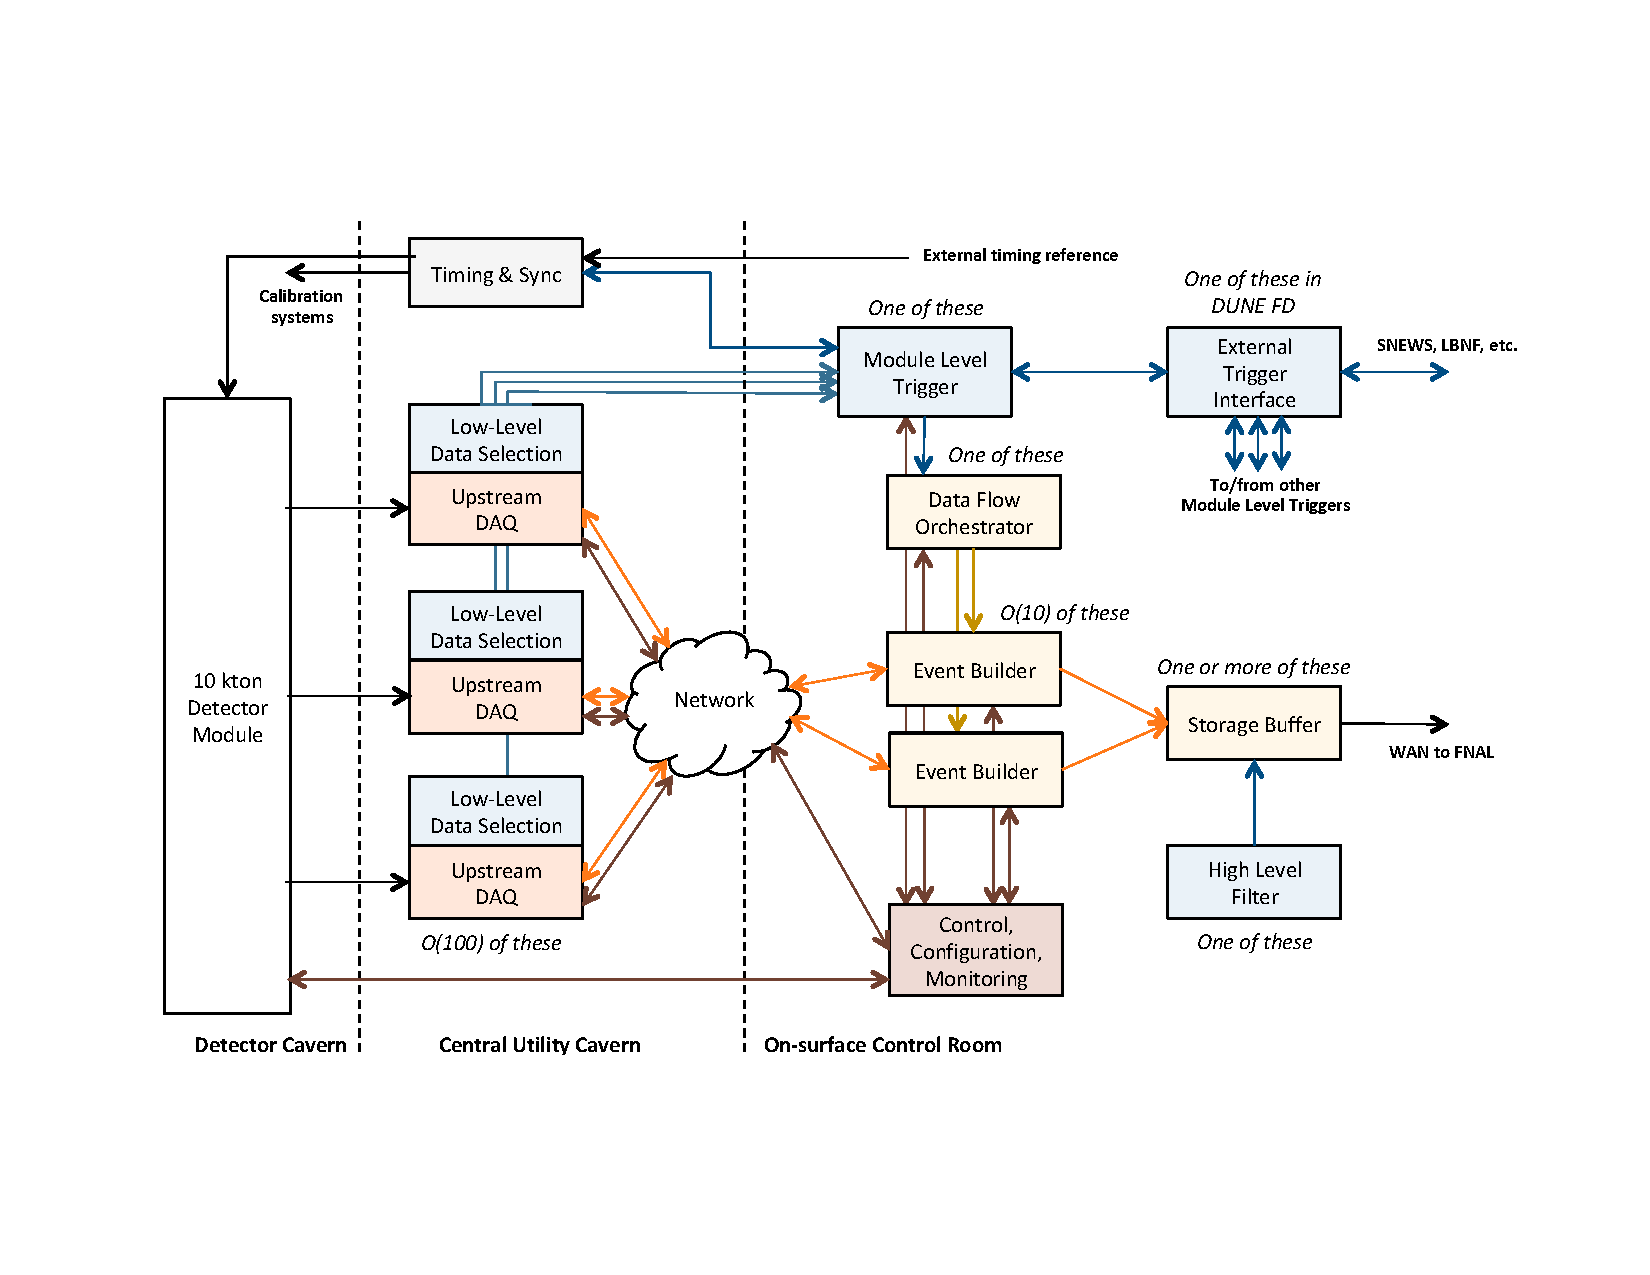
\includegraphics[width=0.8\textwidth,trim=4cm 3cm 4cm 3cm]{daq-layout-2.pdf}
\end{dunefigure}


\subsection{Requirements and Specifications}
\label{sec:fd-daq:requirements}

The \dword{dune} \dword{fd} \dword{daq} system is designed to meet the
\dword{dune} top-level as well as \dword{daq}-level requirements
summarized in Table~\ref{tab:specs:SP-DAQ}. The \dword{daq}-level requirements are
imposed to ensure that the 
system %is capable of 
can record all necessary information for offline 
analysis of data that is associated with on- and off-beam physics events, as directed
by the \dword{dune} physics mission, and with minimal compromise to
\dword{dune}'s physics sensitivity. The requirements must be met following the 
specifications provided in the same table.
Those specifications are
associated with trigger functionality, readout,
and operations and are motivated further in the following subsections.

\subsubsection{How DUNE's Physics Mission Drives the DAQ Design}

The DUNE \dword{fd} has three main physics drivers: neutrino \dword{cpv} and related
long baseline oscillation measurements using the high intensity beam provided
by \fnal, off-beam measurements of atmospheric neutrinos and searches
for rare processes such baryon-number-violating decays,
and detection of neutrinos from a \dfirst{snb} occurring within our galaxy. The
\dword{dune} \dword{fd} \dword{daq} system must facilitate data
readout for delivering on these main physics drivers, while keeping
within physical (space, power) and resource constraints for
the system. In particular, the off-beam measurements require the
continuous readout of the detector, and the lack of external triggers for such
events requires real-time or online data processing, and
self-triggering capabilities. Since the
continuous raw data rate of the far detector module, as received by
the \dword{daq} system, reaches multiple
terabits per second, significant data buffering and processing
resources are needed as part of the design, as specified in
later sections of this chapter.

The \dword{dune} \dword{fd} modules employ two active detector components from which the \dword{daq} system must acquire data: the \dfirst{tpc} and the \dfirst{pds}. The two components access the physics by sensing and collecting signals associated with very different sensing time scales.

Ionization charge measurement by the \dword{tpc} for any given activity in the detector requires a nominal recording of data over a time window of order \SIrange{1}{10}{\milli\second}. 
This time scale is determined by the ionization electron drift speed in \lar and the detector dimension along the drift direction, and is nominally set to \spreadout, corresponding to 2.4$\times$\SI{2.25}{\milli\second}.
The latter (\SI{2.25}{\milli\second}) assumes DUNE's nominal drift electric field of 500~V/cm.
The 2.4 factor assures the capture of ionization information from at
least a full drift before and after the trigger time associated with the
activity. Early commissioning data will be used to evaluate and optimize this nominal readout time.

On the other hand, the \dword{pds} measures argon scintillation light emission, which
occurs and is detected over a timescale of multiple nanoseconds to
microseconds for
any given event and/or subsequent subevent process. Unlike the \dword{tpc},
the \dword{pds} data is zero-suppressed in
the \dword{pds} electronics (see Chapter~\ref{ch:fdsp-pd}). Although
the \dword{pds} system readout sampling frequency is higher than that
of the TPC, the combination of zero-suppression and expected activity
levels are assumed to yield significantly lower data rates than the \dword{tpc}. Therefore, the total raw data volume received by
the \dword{daq} system is expected to be dominated by
the \dword{tpc} data, which is sent out from the front-end electronics as a continuous stream.
 
Figure \ref{fig:daq-rates} provides the expected activity rates in a
single far detector module as a function of true energy associated
with given types of signal.
At low energy ($<$10 MeV), activity is dominated by radiological backgrounds
intrinsic to the detector, and
low-energy solar neutrino interactions. Supernova burst neutrinos,
expected to arrive at a galactic \dword{snb} rate of once per century, 
would span the 10-30 MeV range. At higher energies (generally
above 100 MeV), rates are dominated by cosmic rays, beam neutrino interactions,
and atmospheric neutrino interactions. With the exception of supernova
burst neutrinos, the activity associated with any of these physics
signals is localized in space and particularly in time. Supernova burst
neutrinos on the other hand are characteristically different, as they
can be detected as up to several thousands of neutrino interactions
for a given galactic supernova burst. As such, supernova burst neutrinos
are associated with localized activity that extends over the entirety of the
detector and over multiple seconds. %The arrival time and energy
%distribution of
%neutrinos from a \dword{snb} is model-dependent; as such, the DAQ must
%utilize model-independent approach in selecting \dword{snb} activity.

The nature and rates of these signatures necessitates a \dfirst{daqdsn} strategy that handles two
distinct cases: a localized high-energy activity trigger, prompting an event record readout for
activity associated with a minimum of \SI{100}{MeV} of deposited energy; and an extended low-energy
activity trigger, prompting an event record readout when multiple localized low-energy activity
candidates with low deposited energy each (\SI{10}{MeV} threshold) are found over a short (less than
10 seconds) time period and over the entirety of a \nominalmodsize  module. Because of the high
granularity of the detector readout elements, a hierarchical \dword{daqdss} is employed to
provide data processing and triggering, and facilitate optional data reduction and filtering. 

The \dword{daq}  system is required to yield $>$99\% efficiency for particles depositing $>$100 MeV
of energy in the detector, for localized high-energy triggers; it is also required to yield
sufficient efficiency for low-energy deposition in the detector as needed to yield $>$90\% galactic
supernova burst trigger coverage, for extended low-energy triggers. Galactic coverage is defined as
supernova burst trigger efficiency, weighted by the probability of a galactic \dword{snb} (which
is \dword{snb} distance-dependent).

By offline considerations, the \dword{daq} is required to reduce the
full \dword{fd} data volume for offline permanent storage to  \offsitepbpy.
A far detector composed of four single-phase modules employing a
strategy by which the entire \dword{fd} is read out for \spreadout
given the presence of a localized high energy trigger will be limited
by this offline permanent storage constraint to an average readout rate of \SI{0.3}{\hertz}. 
Strategies will be developed during commissioning and early running that will limit the readout to some subset of the detector module and these are expected to allow an increase in this rate limit by about an order of magnitude.
The instantaneous readout rate can be much higher, for example to accommodate calibrations.
For planning purposes, the \dword{daq} will allot an average rate of \dword{snb} triggers of 1 per month.
Given current understanding of \dword{snb} rates and the $>$90\% expected efficiency for \dword{snb} within \SI{100}{\kilo\parsec}, the vast majority of such triggers will be due to fluctuations of low energy radiological backgrounds and potentially of excess noise.
Such triggers will prompt \snbtime of data from the entire module to be read out.
At this average rate and if saved to offline storage, the \dword{snb}
triggers will lead to production of 1.8 PB/year uncompressed from one
single-phase module. There is nevertheless no requirement to store SNB
data that is deemed, after further offline analysis, to be due to fake triggers.

The capability of recording data losslessly is built into the design
as a conservative measure; a particular concern is charge collection
efficiency and resolution in the case of zero suppression, in particular for TPC
induction wire readout channels.
MicroBooNE is currently investigating the impact of zero suppression
on reconstruction efficiency and energy resolution for low-energy
events \cite{bib:uBsnreadout2019}.
Expected data rates from physics signals of interest, which fit the 30 PB yearly generated volume and trigger rate requirements, are summarized in Table~\ref{tab:sp-daq:rates} and detailed in~\citedocdb{9240} and potential bottlenecks were analyzed in~\citedocdb{11461}.

\begin{dunefigure}[Expected physics-related activity
    rates in one FD module]{fig:daq-rates}{Expected physics-related activity
    rates in a single \nominalmodsize module. \label{sec:fd-daq:rates}
}
  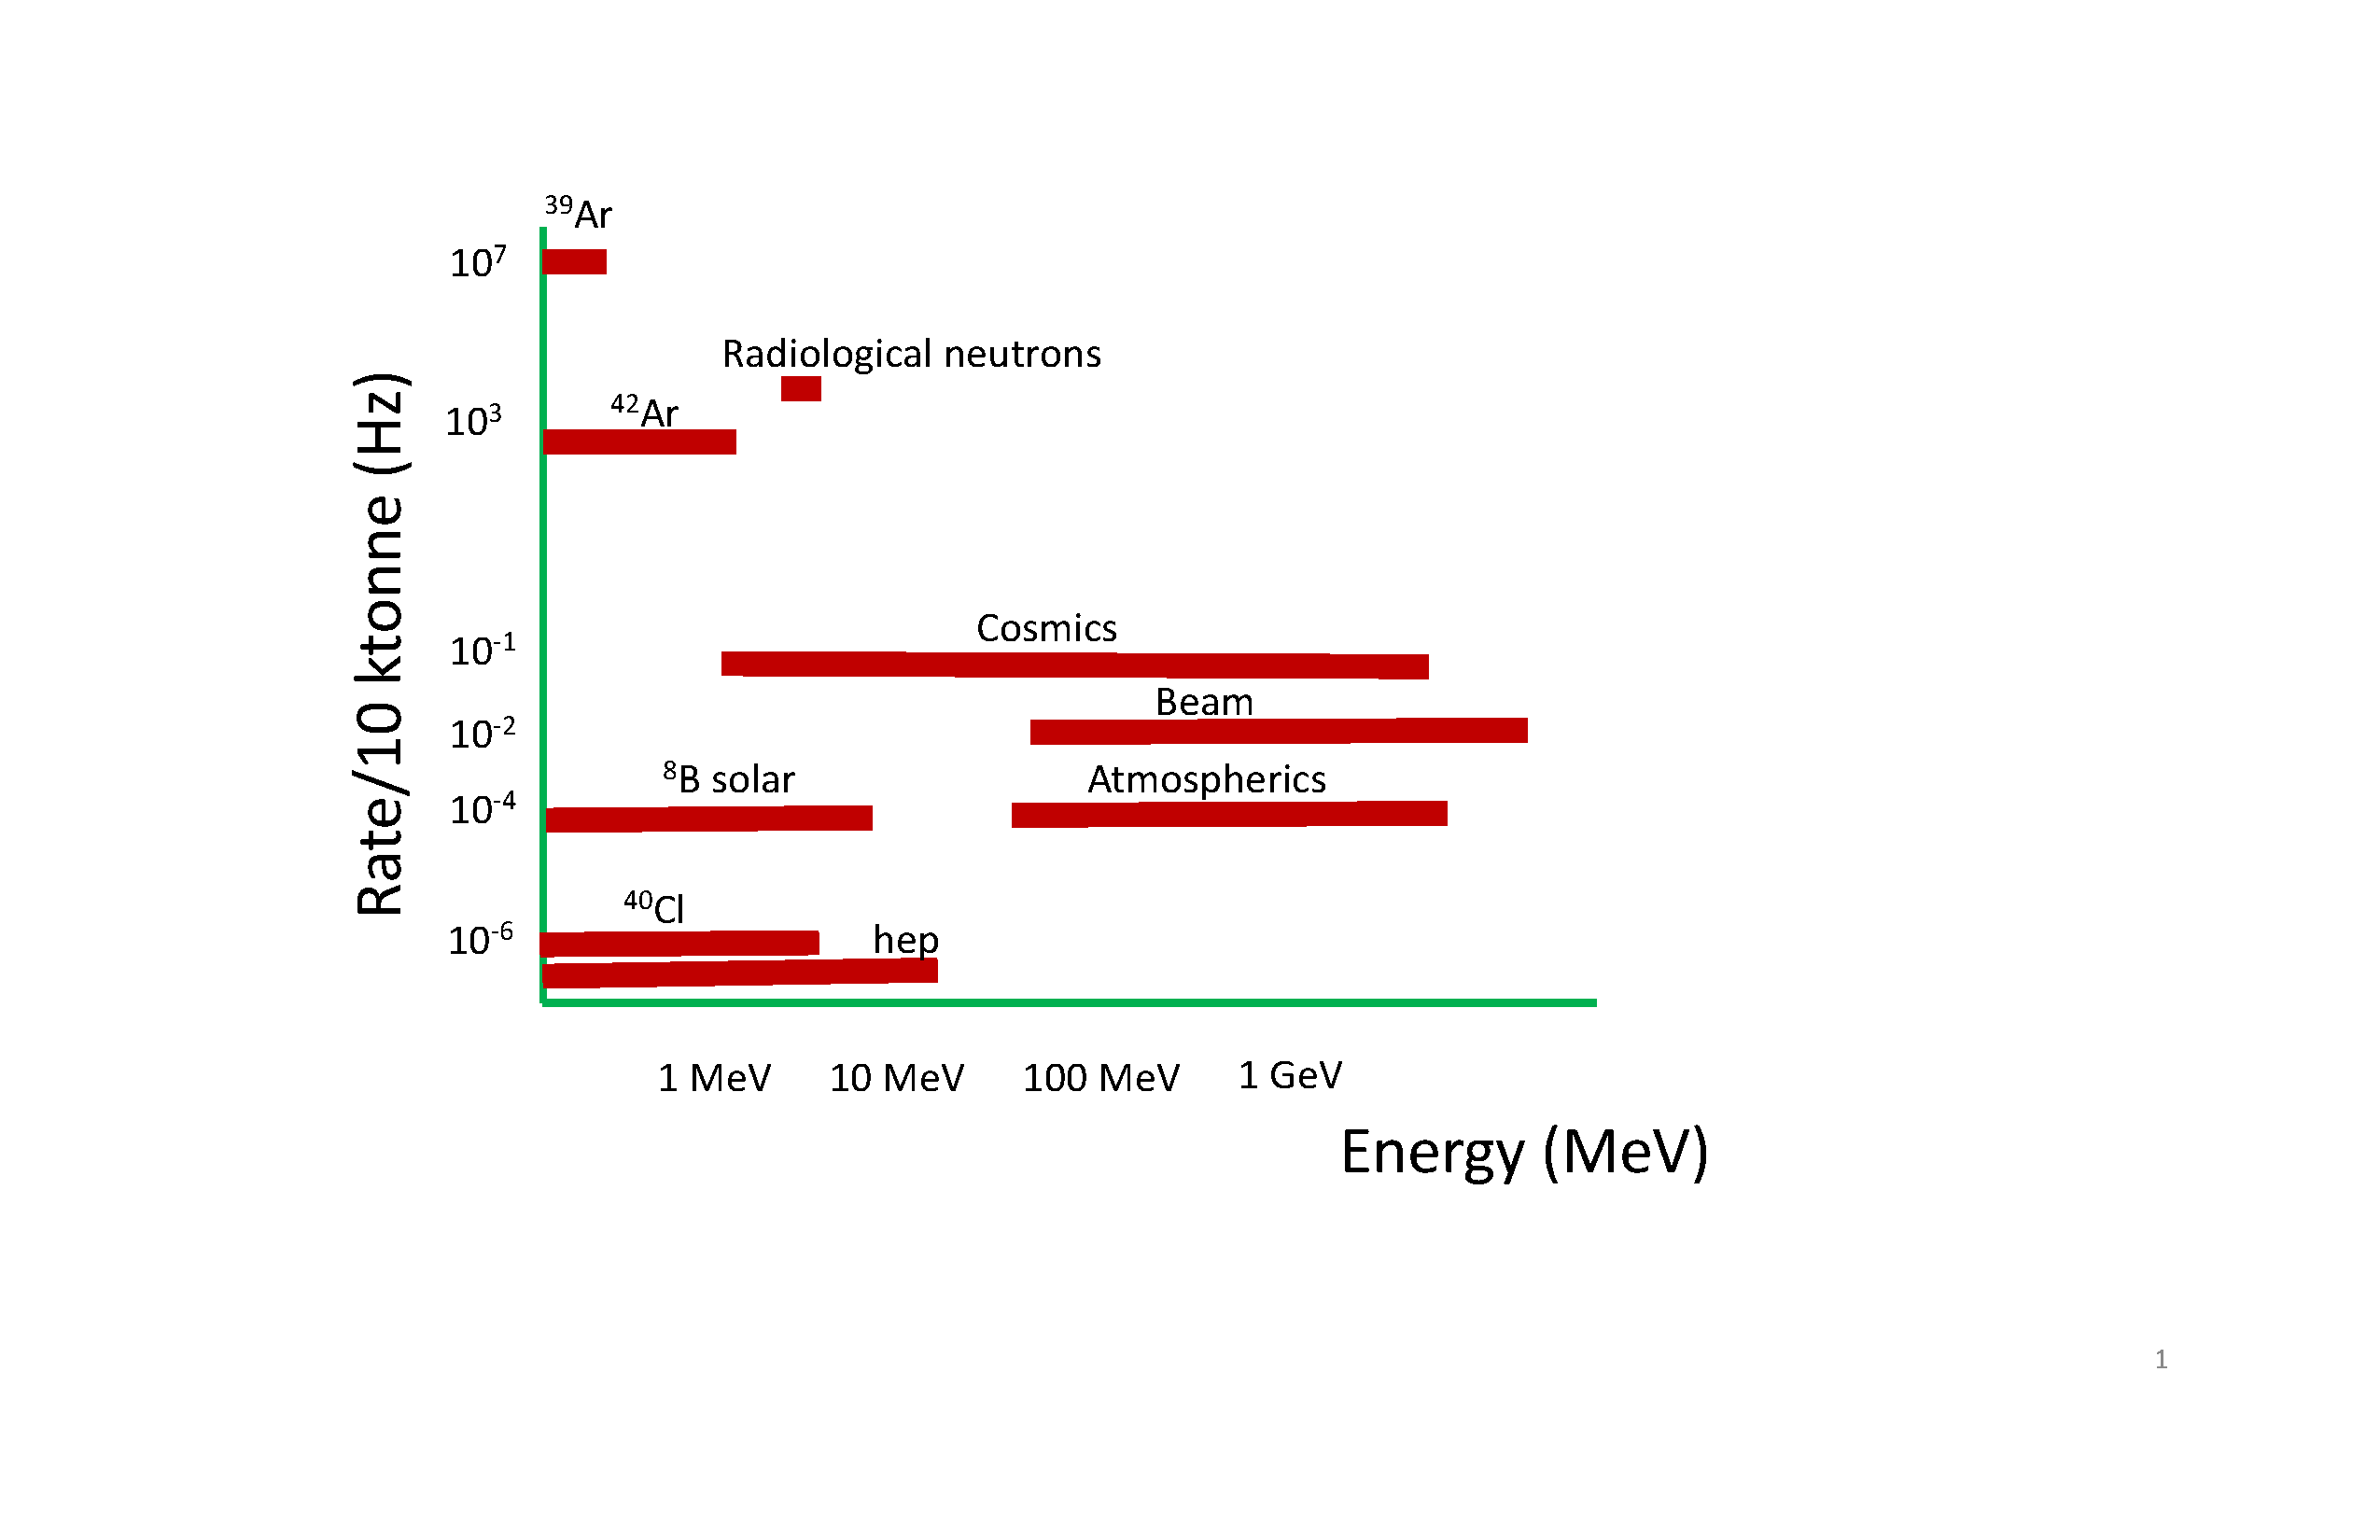
\includegraphics[width=0.7\textwidth,clip,trim=6cm 6cm 10cm 2cm]{daq-event-type-rates-vs-energy.pdf}
\end{dunefigure}

\begin{dunetable} [Expected DAQ Yearly Produced TPC Data Volumes] {p{0.3\textwidth}p{0.1\textwidth}p{0.5\textwidth}} {tab:sp-daq:rates}{Summary of expected data volumes produced yearly for initial single-module running.
    The numbers assume TPC only rates with no compression, and are given for a single
    \SI{10}{\kilo\tonne} module, assuming the parameters listed in Table~\ref{tab:sp-daq:parameters}. (A 2-4x lossless
    compression factor is expected.)
    Trigger primitives (see Section~\ref{sec:sp-daq:design-data-selection}), fake SNB data as well as additional data recorded for detector performance studies and debugging are not foreseen to be stored offline permanently.}
Source                                              & Annual Data Volume & Assumptions \\\toprowrule
Beam interactions                                   & 27 TB              & 10 MeV threshold in coincidence with beam
time, including cosmic coincidence; \spreadout readout \\\colhline
Cosmics and atmospheric neutrinos                   & 10 PB              & \spreadout readout \\\colhline
Radiological backgrounds                            & $<2$ PB            & $<1$ per month fake rate for SNB
trigger; 100s readout\\\colhline
Cold electronics calibration                        & 4 TB               & scaled from \dword{pdsp} experience \\\colhline
Radioactive source calibration                      & 100 TB             & $<10$ Hz source rate; single
APA readout; \spreadout readout \\\colhline
Laser calibration                                   & 200 TB             & 10$^6$ total laser pulses; half the
TPC channels illuminated per pulse; lossy
compression (zero-suppression) on all channels\\\colhline
Random triggers                                     & 60 TB
& 45 per day; \spreadout readout \\\colhline
Trigger primitives and detector performance studies & $<15$ PB           & $^{39}$Ar dominated\\\colhline
\end{dunetable}

Self-triggering on \dword{snb} activity is a unique challenge for the
DUNE \dword{fd}, and an aspect of the design which has never been demonstrated
in a \dword{lartpc}. The challenge with \dword{snb} triggering is two-fold. 
First, the activity of the individual \dword{snb} neutrino interactions
is expected to be of relatively low energy (\SIrange{10}{30}{\mega\electronvolt}),
often indistinguishable from pile-up of radiological background activity in the
detector.  Triggering on an ensemble of \bigo{100} events expected on
average in the case of a galactic supernova burst is therefore
advantageous; however, since this ensemble of events is expected to occur sparsely over the
entire detector and over an extended period of \bigo{10}\si{s},
sufficient buffering capability must be designed into the system to
capture the corresponding signals. 
Furthermore, to ensure high efficiency in collecting \dword{snb} interactions
that, individually, are below low-energy activity threshold, data from
all channels in the detector will be recorded over an extended and contiguous period of
time \bigo{100}\si{s} around every \dword{snb} trigger.

% This file is generated, any edits may be lost.

\begin{longtable}{p{0.14\textwidth}p{0.13\textwidth}p{0.18\textwidth}p{0.22\textwidth}p{0.20\textwidth}}
\caption{Requirements and Specifications Relevant to the for SP-DAQ
  System} \\
  \rowcolor{dunesky}
       Label & Description  & Specification \newline (Goal) & Rationale & Validation \\  \colhline

   \newtag{SP-FD-1}{ spec:min-drift-field }  & Minimum drift field  &  $>$\,\SI{250}{ V/cm} \newline ( $>\,\SI{500}{ V/cm}$ ) &  Lessens impacts of $e^-$-Ar recombination, $e^-$ lifetime, $e^-$ diffusion and space charge. &  ProtoDUNE \\ \colhline
    
   
  \newtag{SP-FD-2}{ spec:system-noise }  & System noise  &  $<\,\SI{1000}\,e^-$ &  Provides $>$5:1 S/N on induction planes for  pattern recognition and two-track separation. &  ProtoDUNE and simulation \\ \colhline
    
   
  \newtag{SP-FD-3}{ spec:light-yield }  & Light yield  &  $>\,\SI{20}{PE/MeV}$ (avg), $>\,\SI{0.5}{PE/MeV}$ (min) &  Gives PDS energy resolution comparable that of the TPC for 5-7 MeV SN $\nu$s, and allows tagging of $>\,\SI{99}{\%}$ of nucleon decay backgrounds with light at all points in detector. &  Supernova and nucleon decay events in the FD with full simulation and reconstruction. \\ \colhline
    
    \\ \rowcolor{dunesky} \newtag{SP-FD-4}{ spec:time-resolution-pds } & Name: Time resolution \\
    Description & The time resolution of the photon detection system shall be less than 1 microsecond in order to assign a unique event time.   \\  \colhline
    Specification (Goal) &  $<\,\SI{1}{\micro\second}$  ( $<\,\SI{100}{\nano\second}$ ) \\   \colhline
    Rationale &   Enables \SI{1}{mm} position resolution for \SI{10}{MeV} SNB candidate events for instantaneous rate $<\,\SI{1}{m^{-3}ms^{-1}}$.  \\ \colhline
    Validation &   \\
   \colhline

   \newtag{SP-FD-5}{ spec:lar-purity }  & Liquid argon purity  &  $<$\,\SI{100}{ppt} \newline ($<\,\SI{30}{ppt}$) &  Provides $>$5:1 S/N on induction planes for  pattern recognition and two-track separation. &  Purity monitors and cosmic ray tracks \\ \colhline
    
   
  \newtag{SP-FD-12}{ spec:hv-ps-ripple }  & Cathode HV power supply ripple contribution to system noise  &  $<\,\SI{100}e^-$ &  Maximize live time; maintain high S/N. &  Engineering calculation, in situ measurement,   ProtoDUNE \\ \colhline
    
    
   \newtag{SP-FD-13}{ spec:fe-peak-time }  & Front-end peaking time  &  \SI{1}{\micro\second} \newline ( Adjustable so as to see saturation in less than \SI{10}{\%} of beam-produced events ) &  Vertex resolution; optimized for \SI{5}{mm} wire spacing. &  ProtoDUNE and simulation \\ \colhline
    
   
  \newtag{SP-FD-16}{ spec:det-dead-time }  & Detector dead time  &  $<\,\SI{0.5}{\%}$ &  Meet physics goals in timely fashion. &  ProtoDUNE \\ \colhline
    
    
   
  \newtag{SP-FD-19}{ spec:adc-sampling-freq }  & ADC sampling frequency  &  $\sim\,\SI{2}{\mega\hertz}$ &  Match \SI{1}{\micro\second} shaping time. &  Nyquist requirement and design choice \\ \colhline
    
    
   \newtag{SP-FD-20}{ spec:adc-number-of-bits }  & Number of ADC bits  &  \num{12} bits \newline ( \num{13} bits ) &  ADC noise contribution negligible (low end); match signal saturation specification (high end). &  Engineering calculation and design choice \\ \colhline
    
   
  \newtag{SP-FD-22}{ spec:data-rate-to-tape }  & Data rate to tape  &  $<\,\SI{30}{PB/year}$ &  Cost.  Bandwidth. &  ProtoDUNE \\ \colhline
    
   
  \newtag{SP-FD-23}{ spec:sn-trigger }  & Supernova trigger  &  $>\,\SI{90}{\%}$ efficiency for SNB within \SI{100}{kpc} &  $>\,$90\% efficiency for SNB within 100 kpc &  Simulation and bench tests \\ \colhline
    
   
  \newtag{SP-FD-25}{ spec:non-fe-noise }  & Non-FE noise contributions  &  $<<\,\SI{1000}{enc} $ &  High S/N for high reconstruction efficiency. &  Engineering calculation and ProtoDUNE \\ \colhline
    
    \\ \rowcolor{dunesky} \newtag{SP-FD-27}{ spec:radiopurity } & Name: Introduced radioactivity \\
    Description & Introduced radioactivity shall be less than that from 39Ar.   \\  \colhline
    Specification &  less than that from $^{39}$Ar \\   \colhline
    Rationale &   Maintain low radiological backgrounds for SNB searches.  \\ \colhline
    Validation & ProtoDUNE and assays during construction  \\
   \colhline

    
   
  \newtag{SP-FD-28}{ spec:dead-channels }  & Dead channels  &  $<\,\SI{1}{\%}$ &  Contingency for possible efficiency loss for $>\,$20 year operation.  &  ProtoDUNE \\ \colhline
    

    \\ \rowcolor{dunesky} \newtag{SP-DAQ-1}{ spec:trigger-high-energy } & Name: Off-beam High-energy Trigger \\
    Description & The detector shall trigger on the visible energy of underground physics events from decays or interactions within the active volume with high efficiency.   \\  \colhline
    Specification &  $>$\SI{100}{\MeV} \\   \colhline
    Rationale &   Driven by DUNE physics mission.  \\ \colhline
    Validation & Simulations  \\
   \colhline

   
  \newtag{SP-DAQ-2}{ spec:DAQ-throughput }  & DAQ storage throughput: The DAQ shall be able to store selected data at an average throughput of 10 Gb/s, with temporary peak throughput of 100 Gb/s.  &  10 Gb/s average storage throughput. 100 Gb/s peak temporary storage throguput per single phase detector module;  &  Average throughput estimated from physics and calibration requirements; peak throughput allowing for fast storage of SNB data ($\sim 10^4$ seconds to store 120 TB of data)  &  ProtoDUNE demonstrated steady storage at $\sim$ 40 Gb/s for a storage volume of 700 TB. Laboratory tests will allow to demonstrate the performance reach. \\ \colhline
    
    
   
  \newtag{SP-DAQ-3}{ spec:trigger-beam }  & Beam Trigger  &  $>$\SI{100}{\MeV} &  Driven by DUNE physics mission. &  Simulations, experience from past and ongoing experiments. \\ \colhline
    
   
  \newtag{SP-DAQ-4}{ spec:trigger-calibration }  & Calibration trigger: The DAQ shall provide the means to distribute time-synchronous commands to the calibration systems, in order to fire them, at a configurable rate and sequence and at configurable intervals in time. Those commands may be distributed during physics data taking or during special calibration data taking sessions. The DAQ shall trigger and acquire data at a fixed, configurable interval after the distribution of the commands, in order to capture the response of the detector to calibration stimuli.  &   &  Calibration is essential to attain required detector performance comprehension. &  Techniques for doing this have been run successfully in MicroBooNE and ProtoDUNE.  \\ \colhline
    
   
  \newtag{SP-DAQ-5}{ spec:trigger-calibration }  & Calibration trigger  &   &  Need to understand detector performance. &  Experience from past and ongoing experiments \\ \colhline
    
   
  \newtag{SP-DAQ-6}{ spec:data-verification }  & Data verification: The DAQ shall check integrity of data at every data transfer step. It shall only delete data from the local storage after confirmation that data have been correctly recorded to permanent storage.  &   &  Data integrity checking is fundamental to ensure data quality &   \\ \colhline
    
    
   
  \newtag{SP-DAQ-7}{ spec:deadtime }  & DAQ Deadtime  &   &  Driven by DUNE physics mission. &   \\ \colhline
    


\label{tab:rec-specs:SP-DAQ}
\end{longtable} 

\subsubsection{Considerations for Design}
\label{sec:fd-daq:considerations}

The \dword{daq} system is designed as a single, scalable system that can
service all \dword{fd} modules. It is also designed on the principle that the
system should be able to record and store full detector data with zero dead
time, applying appropriate data reduction through data selection and
compression; and that it should be evolutionary, taking advantage of the
staged construction for the DUNE \dword{fd}, and thus beginning very
conservatively for the first DUNE \dword{fd} module, and agressively reducing
the design conservatism as further experience is gained with detector
operations. At the same time, it is designed to preserve the possibility of
additional capacity as required. The bulk of processing and buffering of raw
detector data is done underground, in the upstream \dword{daq} and low
level data selection parts of the
system (see Figure~\ref{fig:fd-daq:layout}), with only event building and data
storage kept on surface.

Power, cooling, and space are constrained both in the \dword{cuc} and on surface, limited to \daqpower and \daqracks (out of \cucracks total) in the \dword{cuc} and \surfdaqpower and \surfdaqracks on surface for \dword{daq} for all four \dword{fd} modules.
The underground computing required for the \dword{daq} to service the SP detector module is expected to require less than a quarter of the total power and rack space provided for all four detector modules. 
The hardware for upstream \dword{daq}, low level data selection,
various services, networking, and the timing system, including spares,
all residing in the \dword{cuc}, 
are expected to consume less than \SI{63}{\kilo\watt} and fill less
than 300U of rack space, combined \cite{ale}.

%%% numbers from Alessandro
% - 85 felix servers , 350 W, 2 APAs/host, 2Us - including spares
% - 80 trigger servers, 300 W, 1 U
% - 25 servers for MLT, CCM, others, 200 W, 1 U
% - 18 network units, 150 W, 1 U
% - Timing system, 1000 W


There are five key challenges for the DUNE \dword{fd} \dword{daq} system: 
\begin{itemize}
\item First, the high overall experiment's uptime goal, requires the \dword{daq} to be designed with stringent reliability, fault tolerance and redundancy criteria, aiming at contributing in a negligible way to the overall downtime.

  The \dword{daq} system is fully configurable, controllable, and operable from remote locations, with authentication and authorisation implemented to allow exclusive control. The \dword{daq} provides monitoring of the quality of the detector data and of its own operational status, as well as automated error detection and recovery capabilities.

\item Secondly, the system must be able to evolve to accommodate newly commissioned sub-components as they are installed into a detector module which is under construction. 
  The \dword{daq} must also continue to service existing modules which have reached their operational status while simultaneously accommodating subsequent detector modules as they are installed and commissioned. 
  To support this ongoing variability the \dword{daq} will support operating as multiple independent instances or partitions.

  Partitioning will be supported also within a single detector module, in order to support e.g. special calibration or debugging runs of parts of the detector, which are incompatible with physics data taking settings, while the rest of the detector remains in physics data taking mode. Partitioning, i.e. allowing multiple instances of the \dword{daq} to operate independently with different configurations on different parts of the detector, will also be important during the installation and commissioning phases, to parallelize experts work e.g. for photon detectors and TPC.

\item Thirdly, the \dword{snb} physics requirements necessitate large buffering in the upstream \dword{daq}. 

  The implementation of a buffer element in the upstream \dword{daq} allows
  for the formation and capture of delayed, data-driven data selection
  decisions:
  The trigger accumulates low energy signals over an extended period
  of time while carrying out the \dword{trigdecision}, thus identifying activity compatible with \dword{snb}.
  The specification for the depth of this buffer is determined in
  consultation with physics groups and is driven primarily by the need
  to retain all unbiased data while processing up to \SI{10}{s} of
  data for the \dword{trigdecision}, preceding a \dword{snb} trigger.
  Collecting data containing information on other types of interactions and decays does not pose additional requirements on the upstream \dword{daq} buffer, since the latency to form the required triggers is expected to be well below \SI{10}{s}.

\item Fourthly, the \dword{daq} must support a very wide range of readout windows and trigger rates. This encompasses the acquisition of localized events in both time and space up to the very large and rare \dword{snb} detector-wide readouts over \SI{100}{s}.

\item Finally, the \dword{daq} needs to reduce the volume of data to be permanently stored offline to a maximum of \SI{30}{PB/year}.
  The \dword{daq} system is designed so as to be able to select interesting time windows in which activity was detected, apply lossless compression to data records, as well as filter them to remove unnecessary data regions.

A programmable trigger priority scheme ensures that the readout for the main physics triggers is never or rarely inhibited so as to enable easy determination of the live-time of these triggers. 


\end{itemize}

Table~\ref{tab:sp-daq:parameters} summarizes the important parameters driving the \dword{daq} design. These parameters set the scale of data buffering, processing, and transferring resources which must be built into the design of each \dword{fd} module. 

\begin{dunetable}
[Key DAQ Parameters]
{ll}
{tab:sp-daq:parameters}
{Summary of important parameters driving the \dword{daq} design. The \dword{pds}
  system parameters are under study, but it is expected that the \dword{pds} raw
  data volume that must be handled by the \dword{daq} is an order of
  magnitude smaller than the \dword{tpc} raw data volume.}
Parameter                                          & Value \\ \toprowrule
TPC Channel Count per Module                       & 384,000\\ \colhline
TPC Collection Channel Count per Subdetector (APA) & 960\\ \colhline
TPC Induction Channel Count per Subdetector (APA)  & 1,600\\ \colhline
PDS Channel Count per Module                       & 6000\\ \colhline
PDS Channel Count per Subdetector (PDS per APA)            & 40 \\ \colhline
TPC \dword{adc} Sampling Rate                      & 2 MHz\\ \colhline
TPC \dword{adc} Dynamic Range                      & 12 bits\\ \colhline
PDS \dword{adc} Sampling Rate                      & Under study \\ \colhline
PDS \dword{adc} Dynamic Range                      & Under study \\ \colhline
PDS \dword{adc} Readout Length                     & Under study \\ \colhline
Localized Event Record Window                      & \spreadout \\  \colhline
Extended Event Record Window                       & 100 s\\  \colhline
Full size of Localized Event Record per Module     & 6.5 GB \\  \colhline
Full size of Extended Event Record per Module      & 120 TB\\  \colhline
\end{dunetable}


\subsection{Interfaces}
\label{sec:sp-daq:interfaces}

The \dword{daq} system scope begins at the optical fibers streaming raw digital data from the detector active components
(\dword{tpc} and \dword{pds}), and ends at a wide area network (WAN) interface that
distributes the data from on site at \surf to offline centers off
site. The \dword{daq} also provides common computing and network services for
other \dword{dune} systems, although slow control and safety functions
fall outside \dword{daq} scope.

Consequently, the \dword{dune} \dword{fd} \dword{daq} system interfaces with the \dword{tpc} \dword{ce}, \dword{pds}
readout, computing, \dword{cisc}, and calibration systems of the %\dword{dune}
\dword{fd}, as well as with facilities and underground installation. The
 interface agreements with the \dword{fd} systems 
are listed in Table~\ref{tab:sp-daq:interfaces}, and described
briefly in the following subsections. Interface agreements with
facilities and underground installation are described in Section~\ref{sec:sp-daq:production}.

\begin{dunetable}
[DAQ System Interface Links]
{p{0.3\textwidth}p{0.3\textwidth}p{0.2\textwidth}}
{tab:sp-daq:interfaces}
{Data Acquisition System Interface Links }
Interfacing System & Description & Reference \\ \toprowrule
TPC CE & Data rate and format, number and type of links, timing, inherent noise & \citedocdb{6742}{v6}\\ \colhline
PDS Readout & Data rate and format, number and type of links, timing &  \citedocdb{6727}{v2} \\ \colhline
Computing & Off-site data transfer rates, methods, data file content, disk buffer, software development and maintenance &  \citedocdb{7123} \\ \colhline
CISC & Information exchange, hardware and software for rack and server monitoring & \citedocdb{6790}{v1} \\ \colhline
Calibration & Constraint on total volume of the calibration data; trigger and timing distribution from the \dword{daq} & \citedocdb{7069} \\ \colhline
Timing and Synchronization & Clients, clock frequency, protocols,
transports, accuracy, synchronization precision, monitoring&  \citedocdb{11224} \\ \colhline
Facilities & Detector integration, coordination, cables, racks, safety, conventional facilities, lack of impact on cryo and DSS &  \citedocdb{6988}{v1} \\ \colhline
Installation & Prototyping, planning, transport, underground equipment and activity, safety & \citedocdb{7015} \\ \colhline
\end{dunetable}

\begin{description}
\item[\dword{tpc} \dword{ce}] The \dword{daq} and \dword{tpc} \dword{ce} interface is described in
\citedocdb{6742}. The physical interface is at the \dword{cuc}, where optical links from the \dwords{wib} transfer
the raw \dword{tpc} data to the \dword{daq} \dword{fe} readout (\dword{felix}; see
Section~\ref{sec:daq:design-upstream}). This ensures the \dword{daq} is electrically decoupled from the detector
cryostat. Ten \SI{10}{Gbps} links are expected per \dword{apa}, and have
been specified as 300m OM4 multi-mode fibers from \dword{sfp}+ at the \dword{wib} to
\dword{minipod} on \dword{felix}. (The optical fibers themselves are
the responsibility of the \dword{daq} Consortium.) The data format has been specified
to use a custom communication protocol and no
compression.

\item[\dword{pds} Readout] The \dword{daq} and \dword{pds} readout interface is described in
\citedocdb{6727}. It is anticipated to
be of the form of no more than 150  \SI{10}{Gbps} OM4 fibers from one \dword{fd} module. 
This
is similar to the interface to the \dword{tpc} \dword{ce}, except the overall
data volume is lower by an order of magnitude. The data format has been specified to use
compression (zero suppression) and a custom communication protocol.

\item[Computing] The \dword{daq} and computing interface is described in \citedocdb{7123}.
 The computing consortium
 is responsible for the online areas of WAN connection between \surf and
\fnal providing on order \SI{100}{Gbps} bandwidth, while the \dword{daq} consortium is responsible for disk buffering
to handle any temporary WAN disconnects and the infrastructure needed
for real-time data quality monitoring.  The computing consortium 
is also
responsible for the offline development and operation of the tools for data
transfers to \fnal. The primary
constraint in defining the \dword{daq} and offline computing interface is the
requirement to produce less than \SI{30}{PB/year} 
into final storage at
\fnal. \dword{daq} and
computing consortia are jointly responsible for data
format definition and data access libraries, as well as real-time data
quality monitoring software. The former is specified in the form of a 
data model documented in \citedocdb{7123}.

\item[CISC] The \dword{daq} and \dword{cisc} interface is described in
\citedocdb{6790}. The \dword{daq} provides a network in the \dword{cuc} for \dword{cisc},  operation information and hardware
monitoring information to \dword{cisc}, and power distribution and
rack status units in \dword{daq} racks. The information from \dword{cisc}
feeds back into the \dword{daq} for run control operations.

\item[Calibration] The \dword{daq} and calibration interface is described in \citedocdb{7069}. Two calibration systems are envisioned for the \dword{fd}: a laser calibration system and a neutron generator. 
  Two-way communication between the calibration system and the
  \dword{daq} is needed.  Specifically, the calibration system must
  notify the data selection system, thus informing \dword{trigdecision},
  when activity has been induced in the detector. At the same time, the \dword{daq} must provide input to the calibration system so that it may avoid inducing activity in the detector during certain periods such as during a \dword{snb} readout time or during a beam spill.
This second communication will be initiated by the data selection
system and distributed via the \dword{daqeti} and
subsequently through the
\dword{daq} timing system.


\item[Timing and Synchronization] The timing system of the \dword{dune} \dword{fd} connects with almost all detector systems and with the calibration system and has a uniform interface to each of them. 
  A single interface document \citedocdb{11224} describes all timing interfaces. 

Accuracy of timestamps delivered to  detector endpoints will be $\pm$\SI{500}{\nano\second} with respect to UTC. Synchronization between any two endpoints in the detector will be better than \SI{10}{\nano\second}. Between detector modules, synchronization will be better than \SI{25}{\nano\second}.  
\end{description}

\section{Data Acquisition System Design}
\label{sec:fd-daq:design}

This section begins with an overview of the \dword{daq}
design followed by
descriptions of the subsystem designs and implementation specifics.

\subsection{Overview}
\label{sec:fd-daq:design-overview}

The  \dword{daq} system is composed of five distinct subsystems:
%
(1) upstream \dword{daq} (Section~\ref{sec:daq:design-upstream}),
%
(2) \dfirst{daqdss} (Section~\ref{sec:sp-daq:design-data-selection}),
%
(3) \dfirst{daqbes} (Section~\ref{sec:fd-daq:design-backend}), 
%
(4) \dfirst{daqccm} (Section~\ref{sec:fd-daq:design-run-control}), and
%
(5) \dfirst{daqtss} (Section~\ref{sec:sp-daq:design-timing}).
%
The physical extent of the subsystems
can be specified in reference to Figure~\ref{fig:fd-daq:layout}: the
upstream \dword{daq} and \dword{daqtss}  live underground in the \dword{cuc}; \dword{daqdss} occupies
both underground and above-ground spaces; \dword{daqbes} is above-ground
and includes data flow orchestration, event building and buffering, before distribution of data
to offline; and \dword{daqccm} extends throughout the entire physical layout of the
system, supported on a private network throughout the \dword{daq} system. Each of these subsystems is described in further
detail in the following subsections. 

Front-end readout is carried out by the upstream \dword{daq}, using custom data receiver and
co-processing \dword{fpga}/CPU hardware, all of which is hosted in 80-85 servers in the \dword{cuc}. A
corresponding number of additional servers is responsible for the execution
of subsequent software-based low-level processing of ``trigger
primitives''
generated in the upstream \dword{daq} for the purposes of \dword{daqdsn}. The trigger candidates constructed from trigger primitives are propagated to a central server responsible
for further processing and module-level triggering. The module level
trigger also
interfaces to a second server which is responsible for receiving and
propagating cross-module and external trigger and timing
information. The module level trigger considers trigger candidates and
external trigger inputs in issuing a ``\dword{trigcommand}'' to the \dword{daqbes}
subsystem. The \dword{daqbes} subsystem 
facilitates event building in a few servers and buffering for built
events on non-volatile storage. Upon receiving a \dword{trigcommand}, the \dword{daqbes}
 queries
data from the upstream \dword{daq} buffers and builds that into an ``event
record'', which is temporarily stored as (a number of) files. Event records are optionally processed in a high-level
filter/data reduction stage, which is part of overall data selection,
 prior to event records being shipped to DUNE offline. Pervasively,
 the  \dfirst{daqccm} provides the data taking orchestration
 (Section~\ref{sec:fd-daq:design-run-control}), and the
 \dfirst{daqtss} provides synchronization and synchronous command distribution
 (Section~\ref{sec:sp-daq:design-timing}). Figure~\ref{fig:daq-conceptual-overview}
 provides a conceptual illustration of the overall \dword{daq} system
 functionality.% while Figure~\ref{fig:daq-deployment} illustrates the deployment of the system.
 %, while Figure~\ref{fig:daq-design}
%specifies the design implementation. 

\begin{dunefigure}[DAQ system overview]{fig:daq-conceptual-overview}{Conceptual
   Overview of \dword{daq} System Functionality for a single \nominalmodsize module}
  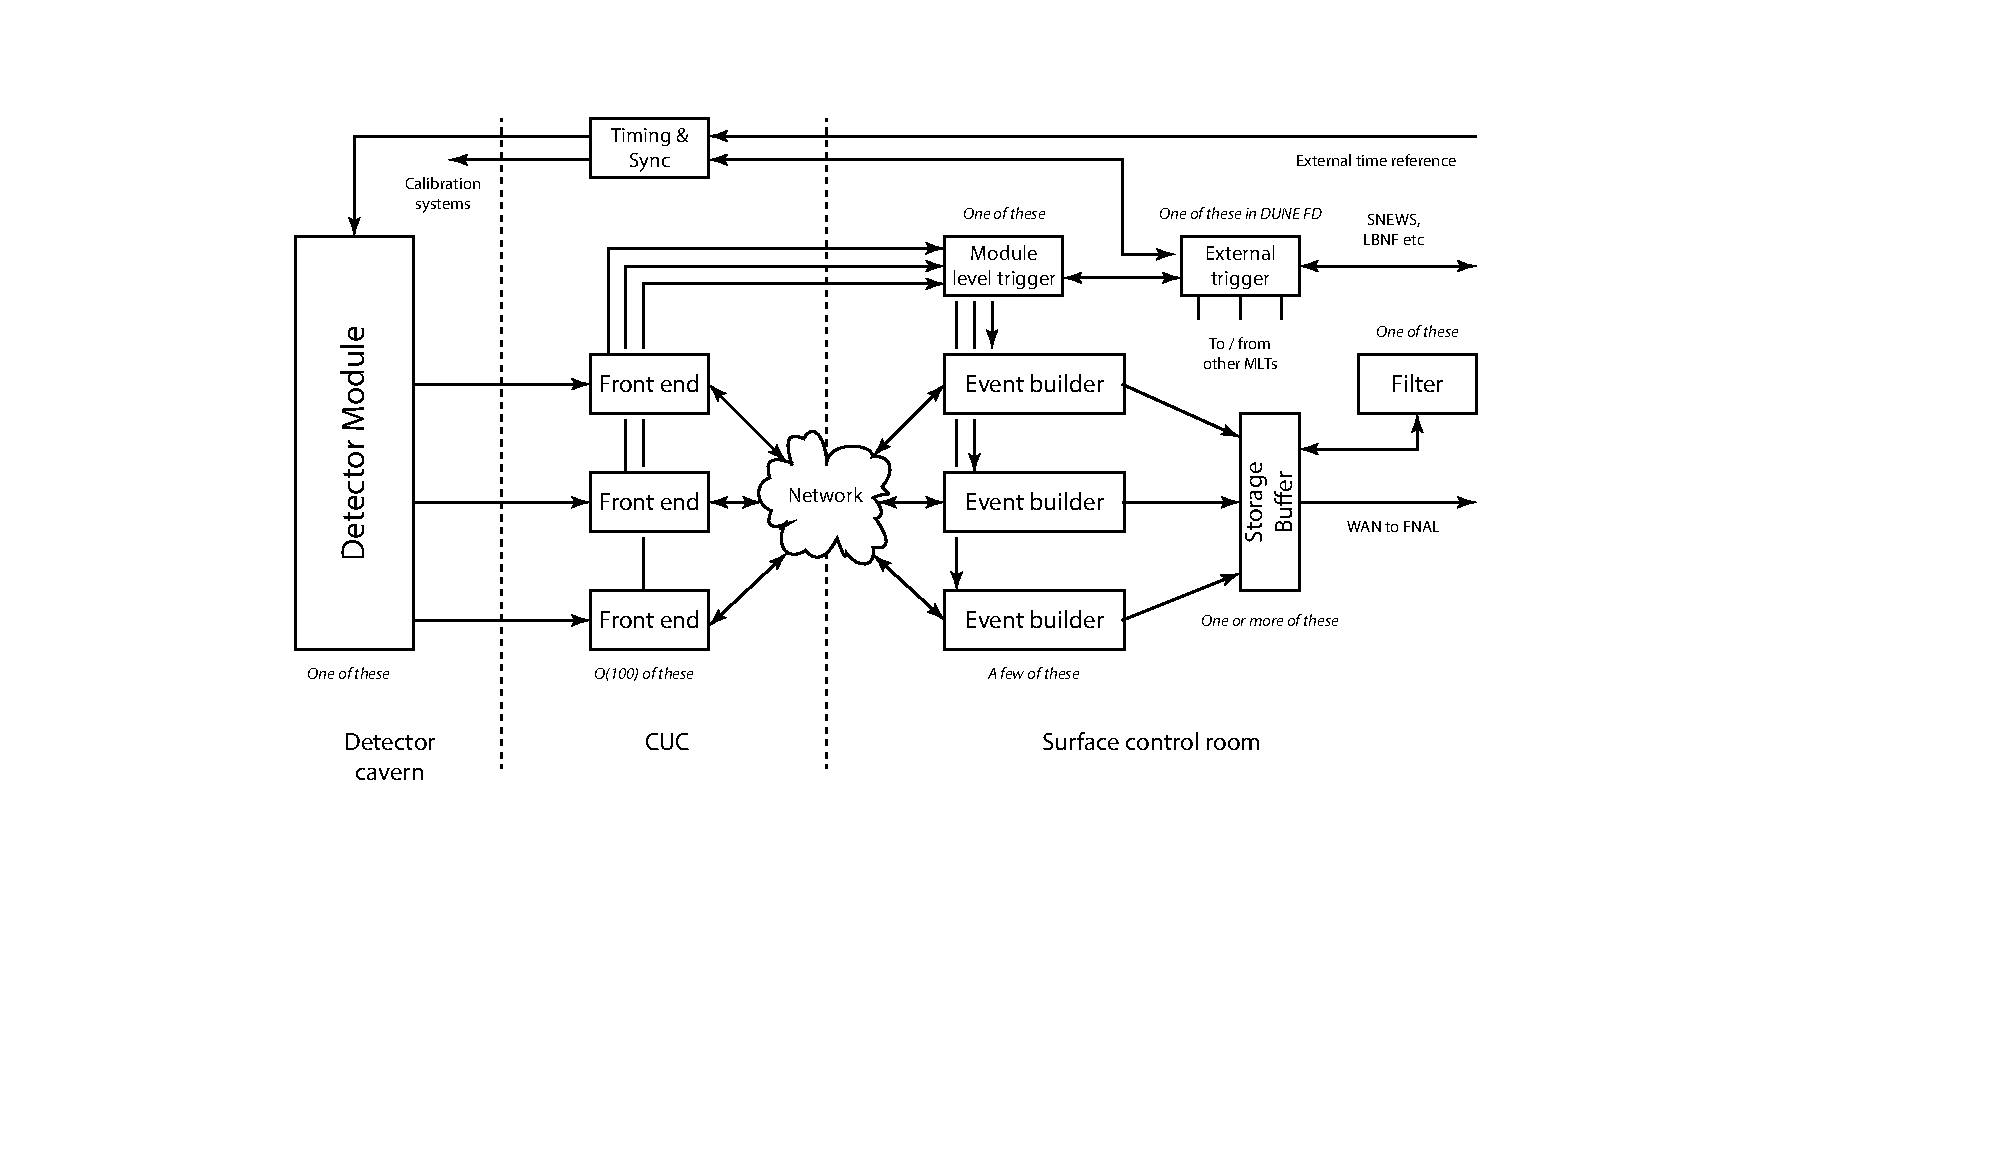
\includegraphics[width=0.9\textwidth]{daq-overview.pdf}
\end{dunefigure}

Key to the implementation of the \dword{daq} design is the requirement that
the system is partitionable. Specifically, the system can operate in
the form of multiple independent \dword{daq} instances, each 
executed across all \dword{daq} subsystems and uniquely mapped among subsystem components. 
More specifically, a given partition may span the entire %up to one
\dword{detmodule} or some subset of it; its extent is configurable at
run start. This ensures continual readout of the
majority of the detector in normal physics data-taking run mode, while
enabling simultaneous calibration or test runs of small portion of the
detector without interruption of normal data-taking. 

\subsection{Upstream DAQ}
\label{sec:daq:design-upstream}

The upstream \dword{daq} provides the first link in the data flow chain of
the \dword{daq} system and is where raw data from detector electronics
is received by the \dword{daq}.
It implements a receiver, buffer, and a portion of low-level data
selection (trigger primitive generation; see Section~\ref{sec:sp-daq:design-data-selection}) as detailed in Figure~\ref{fig:daq:readout}.
It is physically connected to the detector electronics via optical
fiber(s) and buffers and serves data to other \dword{daq} subsystems,
namely the \dword{daqdss} and the \dword{daqbes}.

\begin{dunefigure}[DUNE upstream DAQ subsystem and connections]{fig:daq:readout}{\dword{dune} upstream \dword{daq} subsystem and its connections.}
  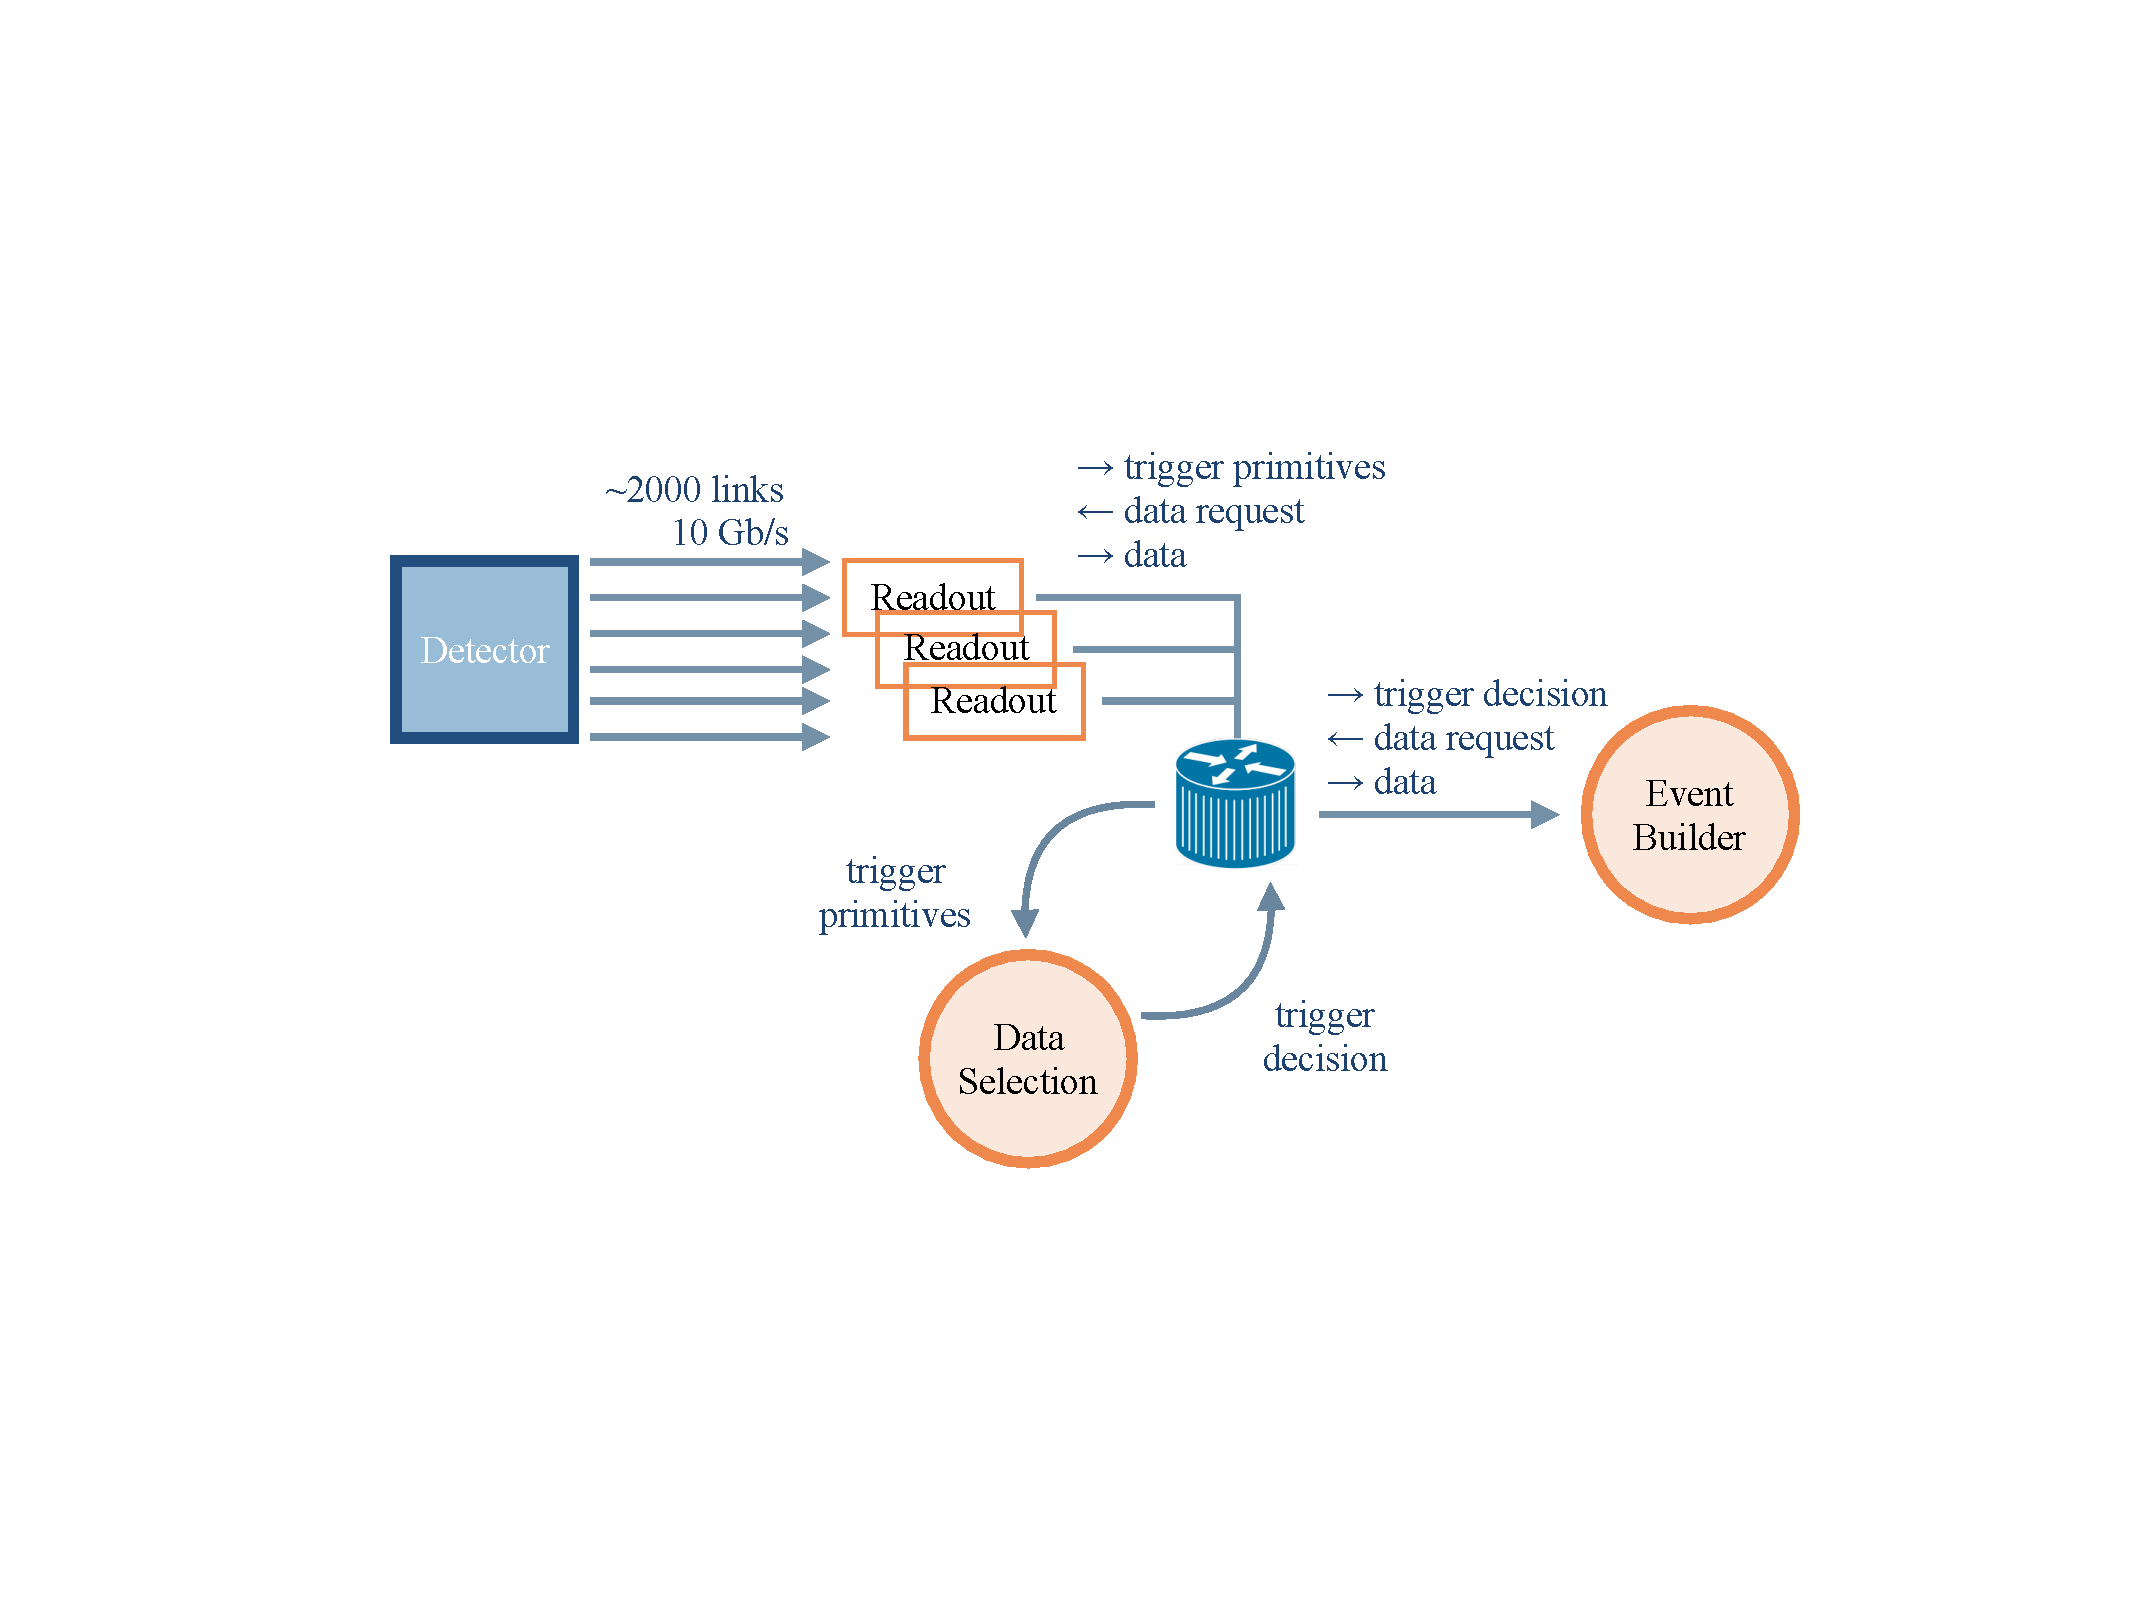
\includegraphics[width=0.8\textwidth]{daq-readout}
\end{dunefigure}

\begin{dunefigure}[Flow diagram of the DUNE upstream DAQ subsystem.]{fig:daq:readout-blocks}{\dword{dune} upstream
    \dword{daq} subsystem functional blocks.}
  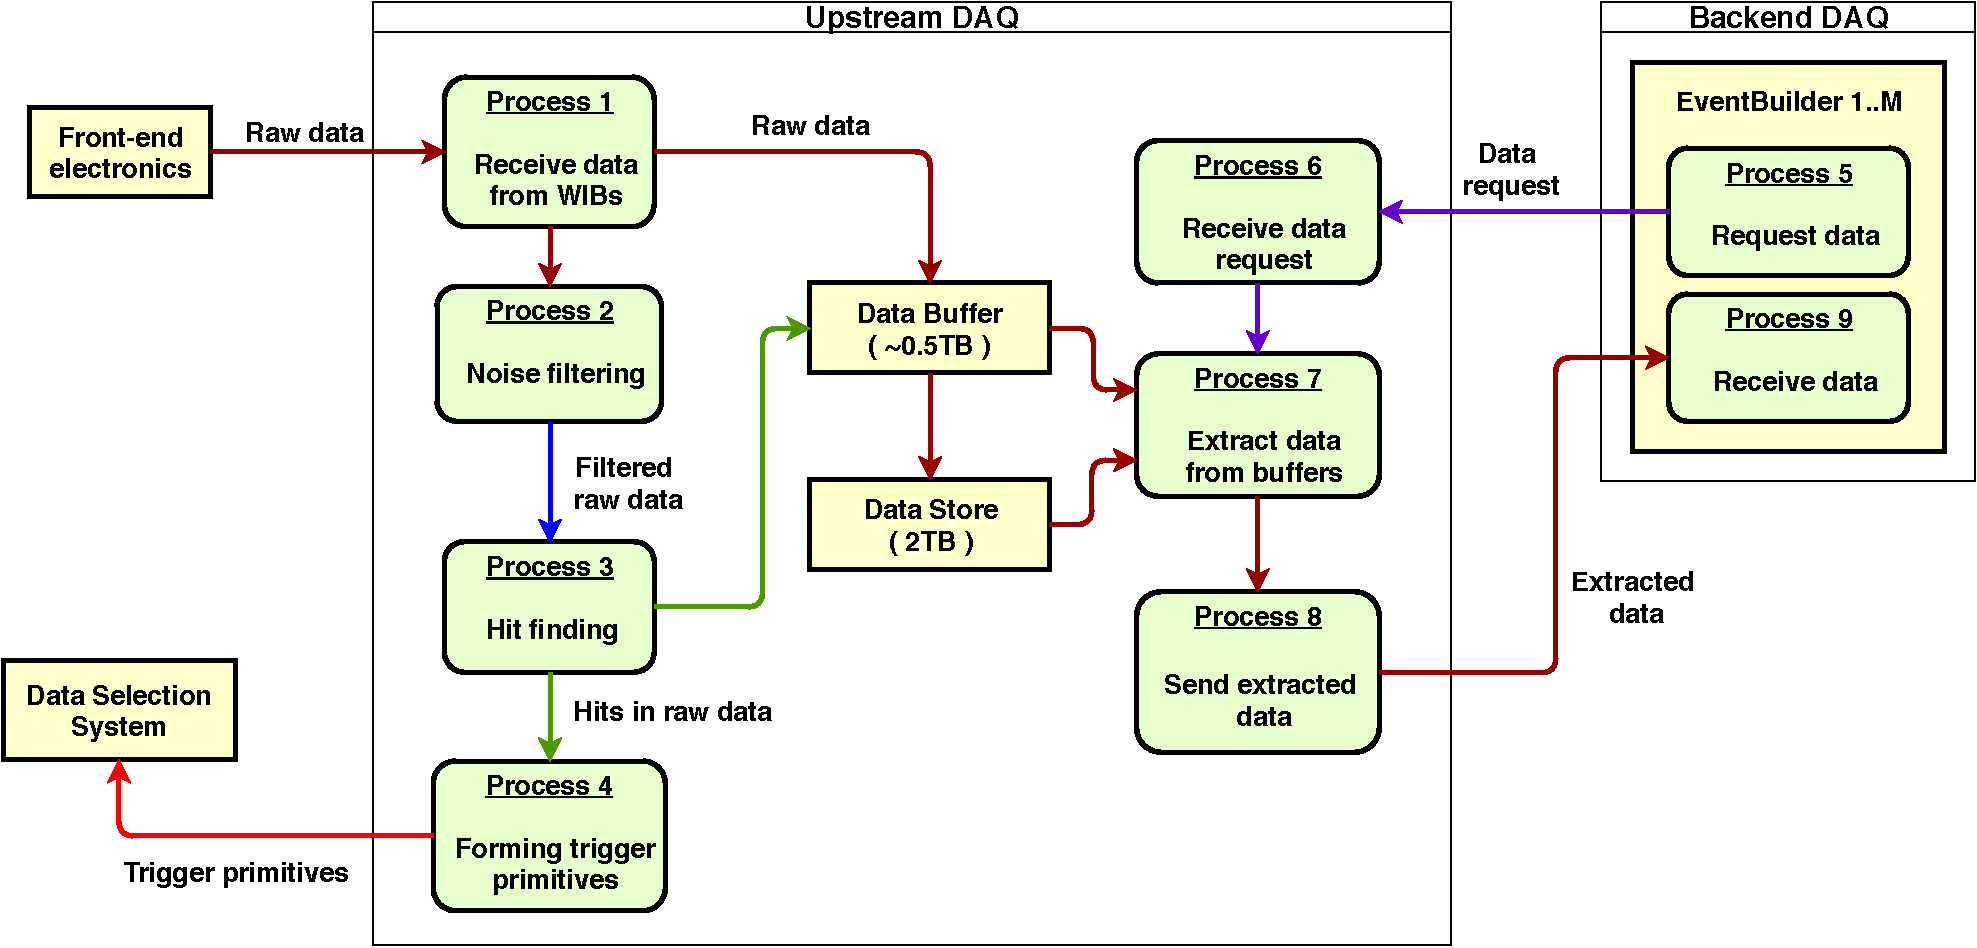
\includegraphics[width=0.8\textwidth]{daq-ud-func-blocks}
\end{dunefigure}

The upstream \dword{daq} system comprises many similar \dwords{daqrou}, each
connected to a subset of electronics from a detector module and
interfacing with the \dword{daq} switched network. In the case of the
\dword{tpc}, 75 functionally identical RU are each responsible for the readout of raw data from two
\dwords{apa}. In the case of the \dword{pds}, up to 8 RU are each responsible for the
readout of raw data from a collection of \dword{pds} subdetectors. 
Each RU is comprised of a \dword{fec} which is a commodity server that hosts a
collection of custom hardware, 
firmware, and software that collectively implement a set of functional blocks.

In the baseline design, used also for system costing, each RU is composed of:
\begin{enumerate}
\item one dual socket multicore 2U server, with two \SI{10}{Gbps} and two \SI{1}{Gbps} ethernet ports for redundant data transmission and control, with at least 256 GB of DDR4 RAM, and sufficient PCIe lanes to host 2 TB of SSD disks,
\item two \dword{felix} cards~\cite{atlas-felix}, each with a PCIe 3.0 x16 interface and supporting 10 \SI{9.6}{Gbps} bidirectional serial optical links,
\item only in case of the TPC readout, four custom-designed co-processor cards mounted onto the two \dword{felix} cards, for additional processing power and data buffering.

\end{enumerate}

The main functional blocks of the upstream \dword{daq} are described below:

\begin{itemize}
  
  \item The physical interface between the detector electronics and the \dword{daq} are 9.6 Gbps
point-to-point serial optical links running a simple (e.g., 8/10 bit encoded) protocol.  For each
\dword{apa} there are ten such links connecting its \dwords{wib} to the \dword{daq}. To reduce space and
power consumption in the \dword{cuc}, high data aggregation is desired. In the baseline design, the
20 fibers from two \dwords{apa} are aggregated into one \dword{fec} with each \dword{apa} connected
to one \dword{felix} FPGA PCIe 3.0 board.  If technology advances sufficiently, a PCIe 4.0 version of
\dword{felix} may be produced to increase the data aggregation such that each board would accept 20
links and a total of 40 links per \dword{fec} would be accomodated. Tests were performed to verify
\dword{om3} and \dword{om4} fibers support \SI{10}{Gbps} links over a run of \SI{300}{\meter}.
Higher-speed fiberoptic links may be employed in order to reduce the number of fibers if run
lengths can be reduced. The \dword{felix} board and firmware was developed initially by and for the
ATLAS experiment and is now proposed or already in use by several other experiments including
\dword{protodune}.
  
  \item The upstream \dword{daq} subsystem provides access to the
\dword{daqdss} and \dword{daqbes} through a commodity switched network as
illustrated in Figure~\ref{fig:daq:readout}. The network communication
protocol is as described in Section~\ref{sec:daq:design-ipc}. The network I/O
is handled by the \dwords{daqrou} via software; dedicated hardware or firmware
development is not required.

\item The data processing functional block is tasked with identifying and forming \dwords{trigprimitive} (see
Section~\ref{sec:sp-daq:design-trigger-primitives}), after a stage of data
reorganization and noise filtering for both the \dword{tpc} and \dword{pds}. \Dwords{trigprimitive} summarize time periods on a channel where the digitized waveform is no longer consistent with noise.
These regions of interest are then used as input to the \dword{daqdss} where they begin the process of forming a \dword{trigdecision}.

In the baseline design this functional block is implemented in \dword{fpga}.
R\&D studies are ongoing to evaluate whether alternative implementations (in GPUs or CPUs) would bring any advantages in terms of flexibility or cost.

\item In \dword{dune}, the upstream \dword{daq} system is in charge of buffering all
detector data until the \dword{daqdss} has issued a \dword{trigcommand}
(see Section~\ref{sec:sp-daq:design-data-selection}) and until the
\dword{daqbes} (Section~\ref{sec:fd-daq:design-backend}) has requested
and received the corresponding selected data. 
In addition, in the case of a \dword{snb} trigger, data received after
the issuing of the trigger must be buffered for a longer period to
avoid loss of data due to any possible downstream
bottlenecks. Localized and extended trigger activity are associated
with two rather different time scales and data throughput metrics, and
those collectively dictate the temporary storage technology and scale. 

The time required to form a \dword{trigdecision} based on localized
activity is expected to be on the order of one second.
Extended triggers present a far more challenging set of buffering
requirements; 
early activity from a \dword{snb} may occur at a rate near that of radiological activity.
Theoretical estimates indicate \snbpretime of integration time may be needed for the
\dword{snb} interaction rate to be deemed significantly enough above
background rate to warrant a trigger.
In order to locate interactions in this low-rate period, the full data rate must be buffered until a \dword{snb} trigger may be formed.
The throughput and endurance required by this buffer is satisfied by RAM technology such as DDR4.

A second challenge in recording data during a \dword{snb} is to assure
essentially 100\% efficiency for collecting the individual, low-energy
interactions during any given \dword{snb} burst. 
To achieve this, the full-stream of data is recorded for a time duration that is expected to cover the time envelope of the burst.
Guided by \dword{snb} models, this duration is chosen to be \snbtime.
This requires extracting as much as \SI{120}{\tera\byte} from the \dword{tpc} upstream \dword{daq} across one single-phase detector module.
It is not cost effective to design the \dword{daq} to extract such
extended data record along the same path as nominal readout, thus
additional buffering is needed.

The technology and scale of this additional buffering must satisfy several requirements. 
Each \dword{daqrou} must accept the full data rate of the portion of the detector module it services.
The media must have sufficient capacity and allow for sufficient extraction throughput so that it is unlikely to ever be too full to accept another extended data record: \SI{4}{\tera\bit/\second} guarantee the ability to store two \dword{snb} events simultaneously.
Furthermore, assuming that, on average, a \dword{snb} trigger condition will be
satisfied once per month, the most optimal technology is
solid-state \dword{nvme} devices, which, at the scale required to provide suitable input bandwidth, can provide a capacity to write the data from several extended activity triggers. The recorded data will be transferred to the \dword{daqbes} system in well under a day.

For both types of activity, the buffering requirements may be reduced by
employing lossless compression to the data prior to it entering the buffer. A
factor of at least two to four compression is expected, based on
MicroBooNE \cite{bib:uBsnreadout2019} 
and \dword{protodune} experience using a modified Huffman encoding of
differential ADC values.  Efforts are currently underway to understand the
costs and technology requirements in exploiting this benefit.

\end{itemize}

Figure~\ref{fig:daq:readout-blocks} shows the flow diagram of data and control messages within the upstream \dword{daq} as well as the main interaction of the upstream \dword{daq} with other subsystems.

\subsection{Data Selection}
\label{sec:sp-daq:design-data-selection}

The \dfirst{daqdsn} subsystem is a hierarchical, online, primarily
software-based system. It is responsible for immediate and continuous processing of a substantial fraction of the entire input data stream. 
This includes data from \dword{tpc} and \dword{pds} subdetectors.
From that input, as well as external inputs provided by
the accelerator and detector calibration systems, the \dword{daqdss} must form a \dword{trigdecision},
which in turn produces a \dword{trigcommand}.
This command summarizes the observed activity that led to the decision
and provides addresses (in channel-time space) of the data in the
upstream \dword{daq} buffers that capture raw data
corresponding to the activity.
This command is sent to and then consumed and executed by the \dfirst{daqbes} as described in Section~\ref{sec:fd-daq:design-backend}. 
It may also be propagated to an \dfirst{etl} stage and from there it may be
distributed to other \dwords{detmodule} or other detector systems
(e.g. calibration) for further consideration.

To facilitate partitioning, the \dword{daqdsn} subsystem will be
able to be instantiated multiple times, and multiple instances will be
able to operate in parallel. Within any
given partition, the \dword{daqdsn} subsystem will also be
informed and aware of current detector configuration and conditions and
apply certain masks and mapping on subdetectors or their fragments in
its decision making. This information is delivered to the
\dword{daqdss} by the \dword{daqccm} system (Section~\ref{sec:fd-daq:design-run-control}).

Following DUNE \dword{fd} and \dword{daq} requirements, the
\dword{daqdss} must select, with sufficiently high ($>$99\%) efficiency, data associated with calibration
signals, as well as beam interactions,
atmospheric neutrinos, rare baryon-number-violating events, and cosmic
ray events that deposit visible energy in excess of 100 MeV. 
It must also select data associated with potential galactic
\dwords{snb} within 100 kpc with $>$90\% efficiency. 
Furthermore, to meet the requirement that the \dword{dune} \dword{fd} maintain
$<$\offsitepbpy to permanent storage, the \dword{daqdss}
must make \dword{daqdsn} decisions in a way that allows the \dword{daq} 
system to effectively reduce its input data by almost four orders of magnitude,
without compromising the above efficiencies.

To meet its requirements, the \dword{daqdss} design follows a hierarchical data selection strategy, where low-level decisions are fed forward into higher-level ones until a module-level trigger is activated. 
The hierarchy is illustrated in
Figure~\ref{fig:daq:data-selection-hierarchy}. 
At the lowest level, trigger primitives are formed on a per-channel basis, and represent, for the baseline design, a ``hit on a wire/channel'' activity summary. 
\Dwords{trigprimitive} are aggregated into \dwords{trigcandidate}, which represent information associated with higher-level constructs derived from trigger primitives, for example ``clusters of hits''. 
\Dword{trigcandidate} information is subsequently used to inform a
module-level \dword{trigdecision}, which generates a \dword{trigcommand};
this takes the form of either a localized high energy trigger or an
extended SNB trigger, and each prompts the corresponding readout of an
event record. Details on the
exact algorithm implementation for trigger primitive, trigger
candidate, and \dword{trigcommand} generation may be found
in~\citedocdb{11215} and~\citedocdb{14522} and references therein. 
Post-event-building, further data selection is carried out in the form
of down-selection of event records, through a high level
filter. Details on a possible post-event-building filtering alforithm
implementation may be found in~\citedocdb{11311}.

This data selection strategy is applicable to both the \dword{pds} and
the \dword{tpc}, operating in parallel up to the module level trigger stage, where \dword{pds} and \dword{tpc} information can be combined to form a module level \dword{trigdecision}. 
Data selection design efforts have taken the approach of validating
and demonstrating a \dword{tpc}-based data selection. Nevertheless,
the data selection design by construction allows an additional
\dword{pds}-based data selection component to be accommodated within
the same design, which will augment data selection capabilities, efficiency and robustness.

The \dword{daqdss} subsystem structure is illustrated in
Figure~\ref{fig:daq:data-selection}. The structure
reflects the three stages of \dword{daqdsn}: (1) low level trigger, which consists of
\dword{trigprimitive} generation (facilitated in upstream \dword{daq}; see
Section~\ref{sec:daq:design-upstream}) and subsequent
\dword{trigcandidate} generation; (2) module level trigger; and (3)
high level filter. Each stage is described in further detail in subsequent
sections. An additional subsystem component is the \dword{daqeti},
which serves as a common interface for the
module level trigger of each of the \dword{fd} \dwords{detmodule} and between
the module level trigger and other systems (calibration,
accelerator and timing system) within a single
\dword{detmodule}. An additional responsibility of the
\dword{daqeti} is to send \dword{snb} triggers
to global coincidence trigger recipients such as \dword{snews}
\cite{snews}, after sufficient confirmation of trigger quality.

\begin{dunefigure}[Data selection strategy and hierarchy]{fig:daq:data-selection-hierarchy}{Data selection
    strategy and hierarchy.}
  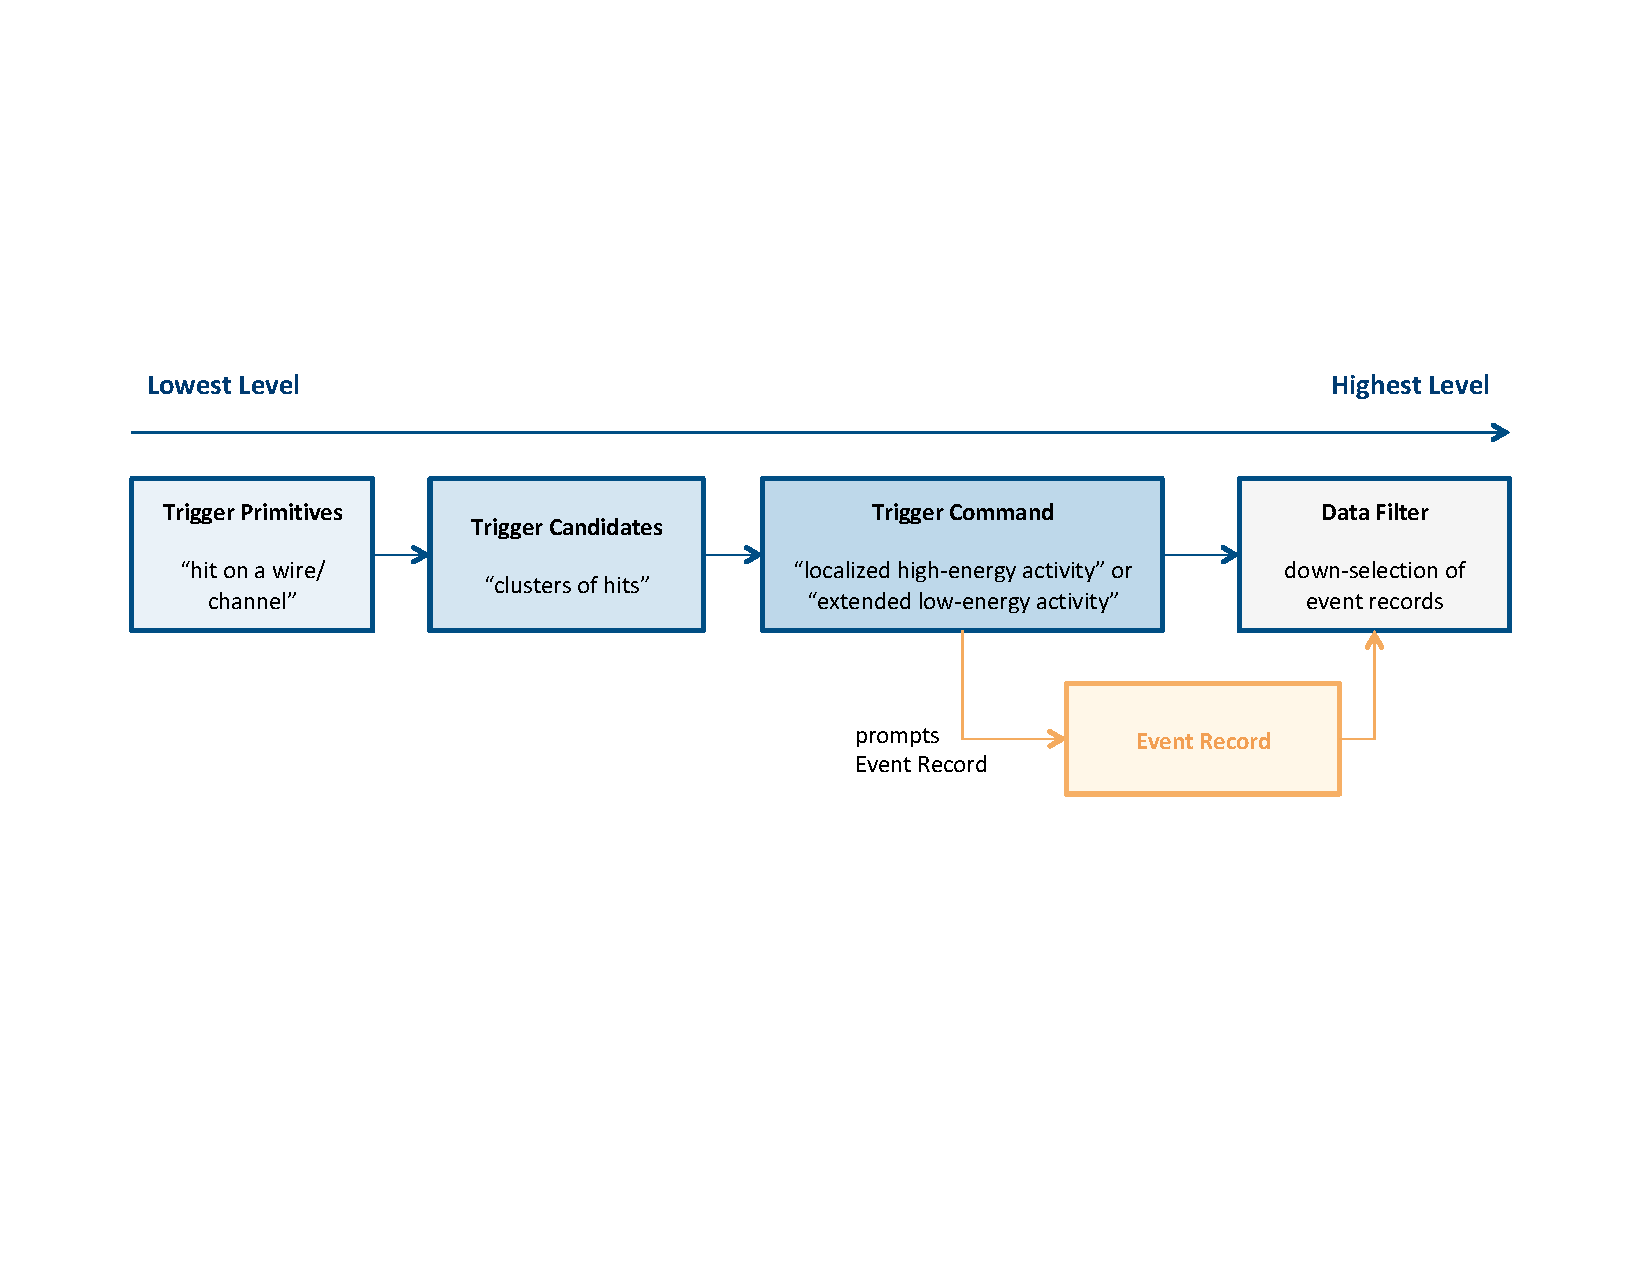
\includegraphics[width=0.9\textwidth, trim=0cm 5cm 0cm 0cm]{DS_hierarchy.pdf}
\end{dunefigure}

\begin{dunefigure}[DUNE DAQ data selection
  subsystem]{fig:daq:data-selection}{Block diagram of the \dword{dune} \dword{daq}
    \dword{daqdsn} subsystem, illustrating hierarchical structure of
    subsystem design, and subsystem functionality and data flow.}
  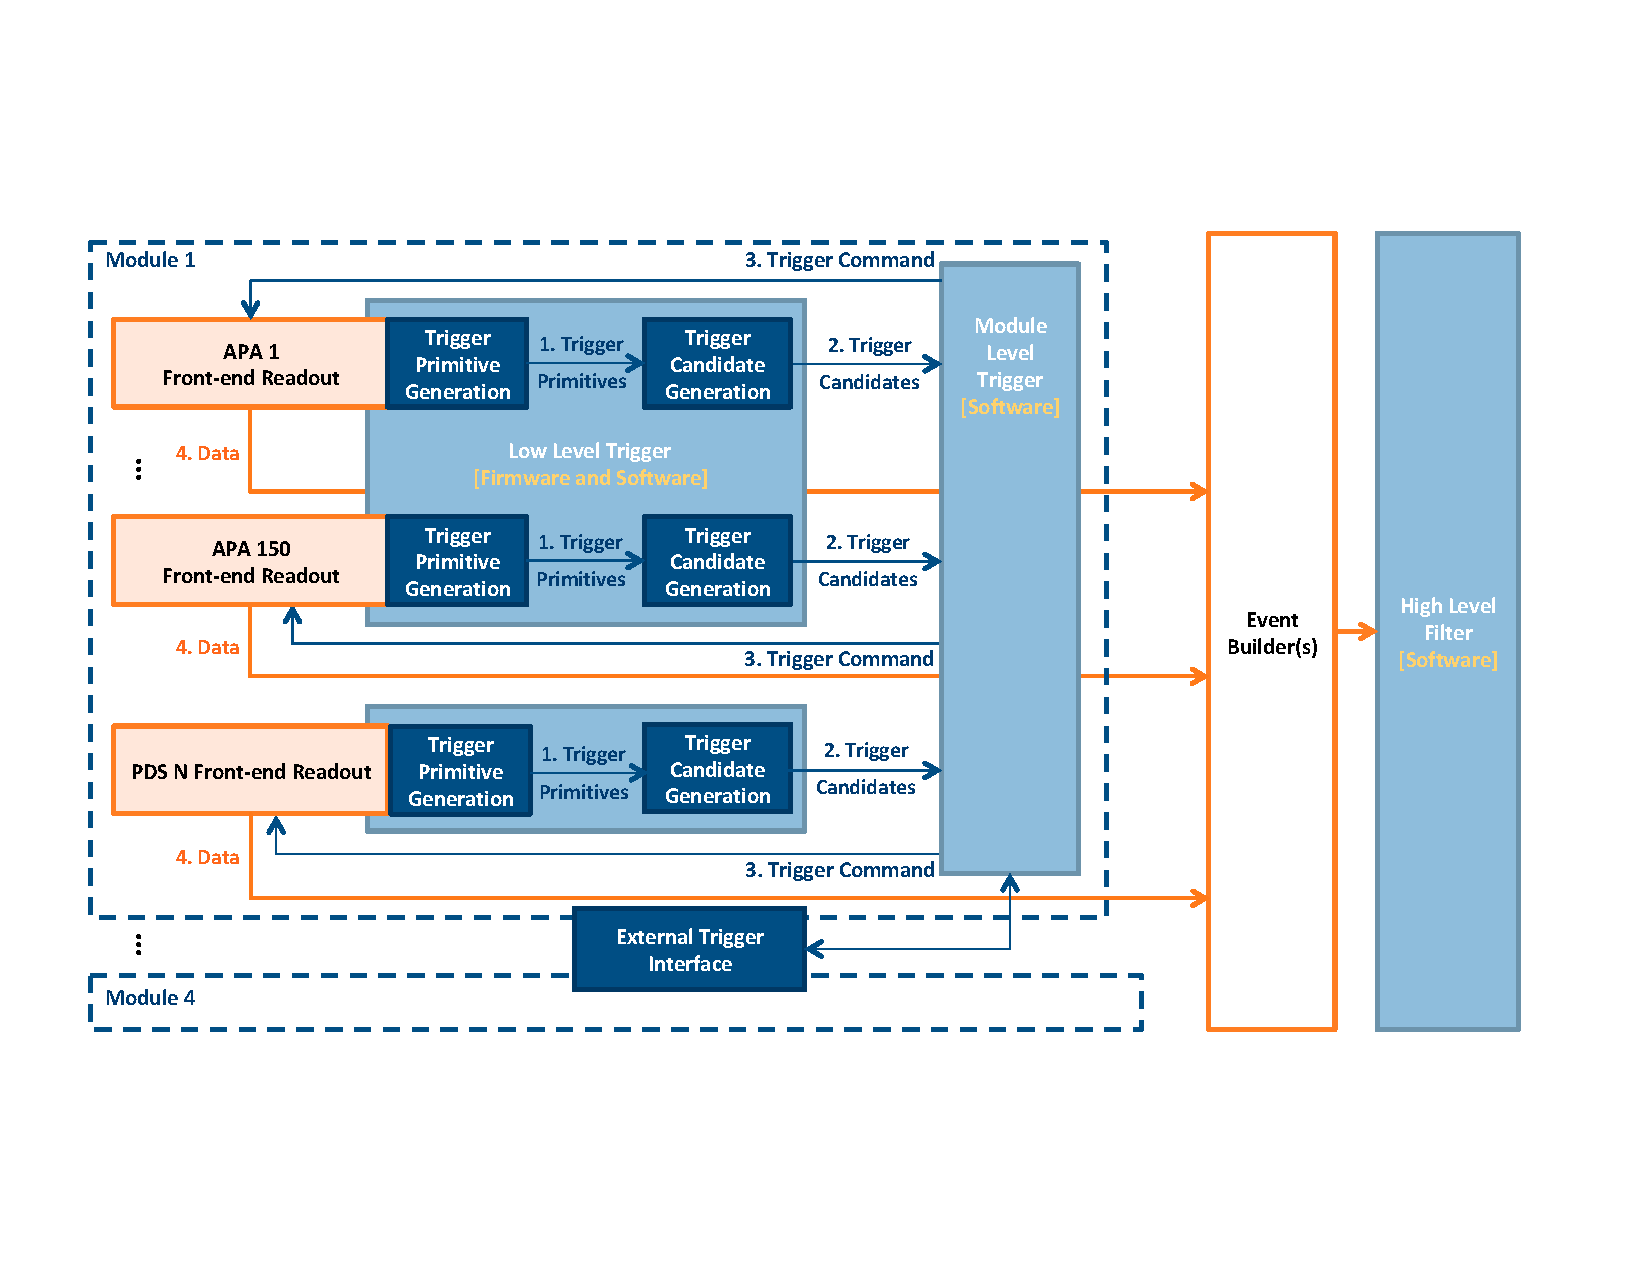
\includegraphics[width=0.95\textwidth, trim=0 2cm 0 0]{DS_summary_2.pdf}
\end{dunefigure}

The first stage of DUNE \dword{fd} operations will trigger on two general
classes of physics, each handled differently at the trigger level:

\begin{description}
\item[High-energy interactions] High-energy interactions include cosmic muons, neutrino beam interactions, atmospheric neutrinos, and nucleon decays. 
  The trigger efficiency for these interactions is explicitly required to be $>$ 99\% for any given particle type (electron,muon, photon, etc.) that has a localized (confined to a few contiguous APAs) visible energy deposition above 100 MeV.
  To achieve this requirement, algorithms for creating high-energy trigger candidates are targeting a trigger effiiency of 50\% at 10 MeV visible energy, thus ensuring >99\% efficiency or better at 100 MeV.
  This type of trigger is referred to as localized high energy trigger. 
  Pushing the high-energy threshold lower could enable detection of diffuse supernova neutrinos and solar neutrinos, if radiological and neutron backgrounds are low enough.

\item[Low-energy interactions] The primary physics target for
  low-energy interactions is a neutrino burst from a nearby supernova. 
  Low-energy trigger candidates (with threshold at or below 10 MeV visible energy) are generated and are input to an ``extended low-energy trigger'' that looks for bursts inconsistent with fluctuations in low-energy background events. 
  The time window for detecting such bursts is tuned to ensure efficiency out to the galactic edge, and the pre-burst buffers are sized to handle the associated latency for detection.

\end{description}


% The first stage of DUNE FD operations will have two general classes of trigger
% decisions that are categorized in terms of the distribution of activity
% in time and channel (mapped to physical) space from which they are derived: 
% \begin{itemize}
% \item Any given far detector module will make a 
%   trigger decision with $>$99\% efficiency for any given particle
%   type (electron, muon, photon, etc.) 
%   that deposits more than 100 MeV of visible energy in a locally
%   confined region (e.g.~a single \dword{apa}, or between two neighboring \dword{apa}s). To achieve this
%   goal, data selection algorithms are targeting a trigger threshold of
%   \SI{10}{\MeV} in visible energy, ensuring $>99$\% efficiency or better
%   at \SI{100}{\MeV}. 
%   This type of trigger is referred to as localized high
%   energy trigger.
% \item Localized activity associated with low deposited energy (as low as below 10 MeV). 
%   Individually, such activity can be caused by neutrinos from burst or relic supernova as well as from the Sun.
%   Collectively, information on these interactions is input to a different type of trigger,
%   referred to as extended low energy trigger, which intended for
%   capturing \dword{snb}.
%   It differs from localized high
%   energy triggers in that it considers the coincidence of localized
%   activity across the entire module, and over an integration period of up to 10
%   seconds.
% \end{itemize}

\noindent Each trigger type prompts readout
of the entire module but over significantly different time
ranges: localized triggers prompt readout of \spreadout event records; extended
triggers prompt readout of \SI{100}{\second} event records. 

Ultimately, each \dword{trigdecision} culminates in a command sent to
the \dword{daqbes} subsystem. 
This command contains all the logical detector addresses and time ranges
required such that an \dword{eb} may properly query the upstream \dword{daq}
buffers and finally collect and output the corresponding detector data
and the corresponding trigger data. To avoid duplication of data
records associated with \dwords{trigcommand} that overlap in readout
record ``space'', the \dword{daqdsn} subsystem must also time-order and
prioritize \dwords{trigdecision}. The details for forming this
command are described next, while the operation of the \dword{daqbes} is
described in Section~\ref{sec:fd-daq:design-backend}.

Viable data selection algorithms for the low level and module level trigger already exist, including
algorithms for a module level \dword{snb} trigger.  It has
been demonstrated through Monte Carlo simulations that the resulting efficiencies meet the above
requirements \cite{bib:docdb11215,bib:docdb14522}. On the other hand, the pipelines of processing required
for \dword{daqdsn} can be executed using different firmware and software
implementations. Development is actively ongoing to demonstrate
and compare performance of different implementations. In satisfying
the philosophy and strategies of the \dword{daq} design, there is built-in
flexibility in defining whether each element of a pipeline executes on
\dword{fpga}, CPU, GPU, or, in principle, some other future hardware
architecture. A purely software implementation of data selection
(including \dword{trigprimitive} generation) is being
implemented for demonstration at \dword{protodune}; it will be then
modified to match the baseline design in which trigger primitives are
generated in upstream \dword{daq} \dword{fpga}.


\subsubsection{Low Level Trigger: Trigger Primitive Generation}
\label{sec:sp-daq:design-trigger-primitives}

A \dword{trigprimitive} is defined nominally on a per-channel basis. In the case of
the \dword{spmod} \dword{tpc}, it is identified as a
collection-channel signal rising above some noise-driven threshold for some minimum period of time (here called a
``hit'').
A \dword{trigprimitive} takes the form of an information packet that 
summarizes the above-threshold waveform information in terms of its
threshold crossing times and statistical measures of its \dword{adc} samples. 
In addition, these packets carry a flag indicating the occurrence of any
failures or other exceptional behavior during \dword{trigprimitive} processing.

% \Dwords{trigprimitive} derived from \dword{tpc} and \dword{pds} data
% are produced in the upstream \dword{daq},
% nominally in \dword{fpga} firmware (\dword{tpc}) and CPU (\dword{pds}), as described in
% Section~\ref{sec:daq:design-upstream}.

Algorithms for generating \dwords{trigprimitive} are under development
\cite{bib:docdb11275}.  Trigger primitive generation proceeds
by establishing a waveform baseline
for a given channel, subtracting this baseline from each sample, maintaining
a measure of the noise level with respect to the baseline, and searching for the waveform to cross a
threshold defined in terms of the noise level. 
The  trigger primitive  (aka ``hit'') is said to span the time period when the waveform is above the noise threshold.
Such algorithms (see, e.g.~\cite{bib:docdb11236}) have been validated
using both Monte Carlo simulations and 
real data from \dword{protodune}. 
Trigger primitive generation performance is summarized in
Section~\ref{sec:sp-daq:design-validation}.

The format and schema of \dwords{trigprimitive} are subject to further
optimization, as they are further tightly coupled with the generation of
trigger candidates, discussed in the following subsection. Nominally,
each trigger primitive comprises the channel address (32 bit), hit
start time (64 bit), the time over
threshold (16 bit), the integral ADC value (32 bit), an error flag (16
bit), and possibly also
the waveform peak (12 bit) associated with the hit. 
As such, 20-22 bytes provides a generous data
representation of \dword{trigprimitive} information. 
The \dword{trigprimitive} rate will be dominated by the rate of decay of naturally occurring
$^{39}$Ar, which is about \SI{10}{\mega\hertz} per module.
This leads to a detector module \dword{trigprimitive} aggregate rate of
\SI{200}{\mega\byte/\second}.
The subsequent stage of the \dword{daqdsn} must continuously absorb and process this
rate providing trigger candidates as described next.

\subsubsection{Low Level Trigger: Trigger Candidate Generation}

At the trigger candidate generation stage of the low level trigger,
\dwords{trigprimitive} from individual, contiguous fragments of the
detector 
module are cross-channel and time correlated, and further selection
criteria are applied. This may result in the
output of trigger candidates. 
More specifically, once activity is localized in time and channel
space, it is
possible to apply a rough energy-based threshold based on the combined
metrics carried by the cross-correlated \dwords{trigprimitive};
satisfying this criteria defines a trigger candidate. 

A trigger candidate packet carries information about all the trigger
primitives that were used in its formation. 
In particular, it provides a measure of the total activity represented
by these primitives, as well as a measure of their collective time and channel
location and extent within the module.
These measures are used downstream by the module level trigger, 
as described more in the next section.

While the selection applied in the previous stage (trigger primitive
generation) is driven by a measure of noise, at trigger candidate
generation stage, prior to applying any thresholds, the rate is driven by
background activity.  
In particular, $^{39}$Ar decays would provide \SI{50}{\kilo\hertz} of
trigger candidates per \dword{apa} face if the threshold was set very low, ie at
\SI{0.1}{\MeV}.
Next, activity from the $^{42}$Ar decay chain would be substantial for a
threshold below \SI{3.5}{\MeV}.
Nominally, individual candidates, or groups of candidates nearby in
detector space and time, with measures of energy greater than these two
types of decays, will be passed to the module level trigger. 

This stage of data selection is implemented 75 (\dword{tpc}) plus 8
(\dword{pds}) CPU servers, which receive the trigger primitive stream from the upstream \dword{daq} and distribute trigger candidates to the module level trigger
stage, described next, via the \SI{10}{Gbps} \dword{daq} network. Studies are underway to demonstrate CPU
resource utilization and latency, as are efforts to demonstrate online trigger candidate generation
at \dword{protodune}. Trigger candidate generation performance is summarized in
Section~\ref{sec:sp-daq:design-validation}. 

%Additional studies are expected but nominally individual candidates, or
%groups of candidates nearby in detector space in time, with measures of
%energy greater than these two types of decays will be passed with little
%or no prescaling.


\subsubsection{Module Level Trigger}
\label{sec:daq:mlt}

Data selection is further facilitated as \dwords{trigcandidate} are consumed
by the module level trigger in order to form the ultimate trigger
decision which prompts the readout of data records from buffers kept by the upstream \dword{daq}. 
The physical (channel and time) location, extent as well as the energy measure of the
candidates are used at this stage to categorize the activity in terms
of a localized high energy trigger or an extended low energy trigger. 
Specifically, $N$ isolated, low energy candidates found in coincidence
over the integration period of up to 10 seconds across the full \dword{detmodule}
indicate the latter; individual high energy candidates, found
otherwise, indicate the former.

When a particular condition in a category is satisfied, the trigger
decision is made and a \dword{trigcommand} is formed. 
The \dword{trigcommand} packet includes information of the candidates (and primitives)
that were used to form it. 
The decision also provides direction as to what set of detector subcomponents
are to be read out and over what time period (localized or extended as described above). 
The module level trigger publishes a stream of \dwords{trigcommand} and the primary subscriber is expected to be the \dword{daqdfo} of the \dword{daqbes} as described in Section~\ref{sec:fd-daq:design-backend}.

The module level trigger is implemented in \bigo{1} CPU server (with 100\%
redundancy), which
receives the trigger candidate stream from the low level trigger stage
of the data selection and distributes \dwords{trigcommand} to the
\dword{daqbes} via the 10 Gbps \dword{daq} network. Studies are
underway to demonstrate CPU resource utilization and latency, as are
efforts to demonstrate online \dword{trigcommand} generation at \dword{protodune}.
\Dword{trigcommand} generation performance is summarized in
Section~\ref{sec:sp-daq:design-validation}.

\subsubsection{External Trigger Interface}

The \dfirst{daqeti} provides a loose coupling between the
\dwords{mlt}, sources of external information such as beam spill times
and information to or from components of \dword{dune} \dword{fd} calibration systems. 

As an interface between \dwords{mlt}, it is responsible receive and distribute information about module-level \dword{snb} \dwords{trigcommand}.
This allows any detector module which alone may not have satisfied a \dword{snb} trigger requirement to nonetheless perform a \dword{snb} readout.
The \dword{daqeti} is also responsible for forming a coincidence between module-level \dword{snb} \dwords{trigcommand} and publishing the results, e.g.~for consumption by the \dfirst{snews}.

The \dword{daqeti} also receives information about beam spill times from the accelerator.
These times can drive a model of the beam timeline to predict when
beam spills and consequently beam-related interactions are expected to occur. 
These predictions can then be sent to the \dwords{mlt} so that they
may either alter \dword{trigdecision} criteria or merely include the
information in contemporaneous \dwords{trigdecision}. The beam time information can also be distributed to components of the calibration system so that they may avoid producing activity in the detector that may interfere with activity from beam neutrinos.

The module level trigger is implemented in \bigo{1} CPU server (with 100\%
redundancy), with 10 Gbps networking and interfacing hardware components (White
Rabbit) for timing and external trigger signal I/O.

\subsubsection{High Level Filter}
\label{sec:fd-daq:design-data-reduction}

The last processing stage in the \dword{daqdsn} subsystem is the
high level filter, which resides in the \dword{daqbes}.
The high level filter acts on triggered, read out, and aggregated data. 
It therefore serves primarily to down-select and thus
limit the total triggered data rate to offline storage, thereby keeping 
efficiency high in collecting information on activities of interest,
while maintaining low selection and content bias, and reducing the output data
rate. It may do so via 
further filtering, lossy data reduction, and/or further event
classification.
As it benefits from operating on relatively low-rate data it can accommodate a higher level of
sophistication in algorithms for \dword{daqdsn} decisions.

More specifically, the high level filter may further reduce the rate of data output to offline storage by
applying refined selection criteria which may otherwise be prohibitive
to apply to the pre-trigger data stream.  For example, instrumentally-generated signals (e.g.~correlated noise)
may produce trigger candidates that can not be rejected by the module
level trigger and if left unmitigated may lead to an undesirably high
output data rate. 
Post processing the triggered data may allow reducing this unwanted
contamination.
% I (bv) don't agree with this next statement.
Furthermore, it can also reduce the triggered data set by further identifying
and localizing interesting activity. A likely candidate hardware
implementation of this level of \dword{daqdsn} is a GPU-based system
residing on surface at SURF.

To fully understand how much and what type of data reduction may be
beneficial, simulation studies are ongoing \cite{bib:docdb11311} and will
necessarily have to be
validated with initial data analysis after
first DUNE \dword{fd} operation. Development efforts are also being
carried out to determine the scale of 
processing required by the \dword{fd}.


\subsection{Back-End DAQ}
\label{sec:fd-daq:design-backend}

The  \dfirst{daqbes} is responsible for moving data of interest identified by the data-selection system from the readout \dword{daq} buffers, serving them to the High-Level Filter and storing the filtered data into the output buffer, from where they will be transferred to permanent storage off-site.

The \dword{daqbes} system accepts \dwords{trigcommand} produced by the \dfirst{daqdss} as described
in Section~\ref{sec:sp-daq:design-data-selection}.  It queries the upstream \dword{daq} buffers and
accepts returned data as described in Section~\ref{sec:daq:design-upstream}. Finally, it records
\dwords{trigcommand} and the corresponding detector data to the output storage buffer.

The principal components of the \dword{daqbes} are the \dfirst{daqdfo}, \dfirst{eb} and the output
storage buffer (OB) in Figure~\ref{fig:fd-daq:layout}.

% The functionality of the \dfirst{daqbes} is comprised of the \dfirst{daqdfo}, \dfirst{eb} and storage buffer blocks in Figure~\ref{fig:fd-daq:layout}. It accepts \dwords{trigcommand} produced by the \dfirst{daqdss} as described in Section~\ref{sec:sp-daq:design-data-selection}. 
% It queries the upstream \dword{daq} buffers and accepts returned data as described in Section~\ref{sec:daq:design-upstream}. Finally, it records \dwords{trigcommand} and the corresponding detector data to the output storage buffer. After application of the high level filter, the data is finally transferred to \fnal for offline storage.

\subsubsection{Data Flow Orchestration}

The \dword{eb} stage is implemented as a pool of redundant \dword{eb} processes to maximize the system tolerance to faults and to handle the readout of long SNB events in parallel to nominal readout requests. This asynchronous, parallel readout will be coordinated by a \dword{daqdfo}.  Its operation is illustrated in Figure~\ref{fig:daq:backend} and is discussed here:

% To minimize the latency in the readout of the data from the upstream
% \dword{daq} buffers, the \dword{daqbes} will support parallel readout of event
% records into a pool of \dword{eb} processes.  This asynchronous, parallel readout will be coordinated by a \dword{daqdfo}.  Its operation is illustrated in Figure~\ref{fig:daq:backend} and is discussed here:

\begin{dunefigure}[DUNE DAQ back-end operation]{fig:daq:backend}{Illustration of \dword{dune} \dword{daqbes} operation.}
  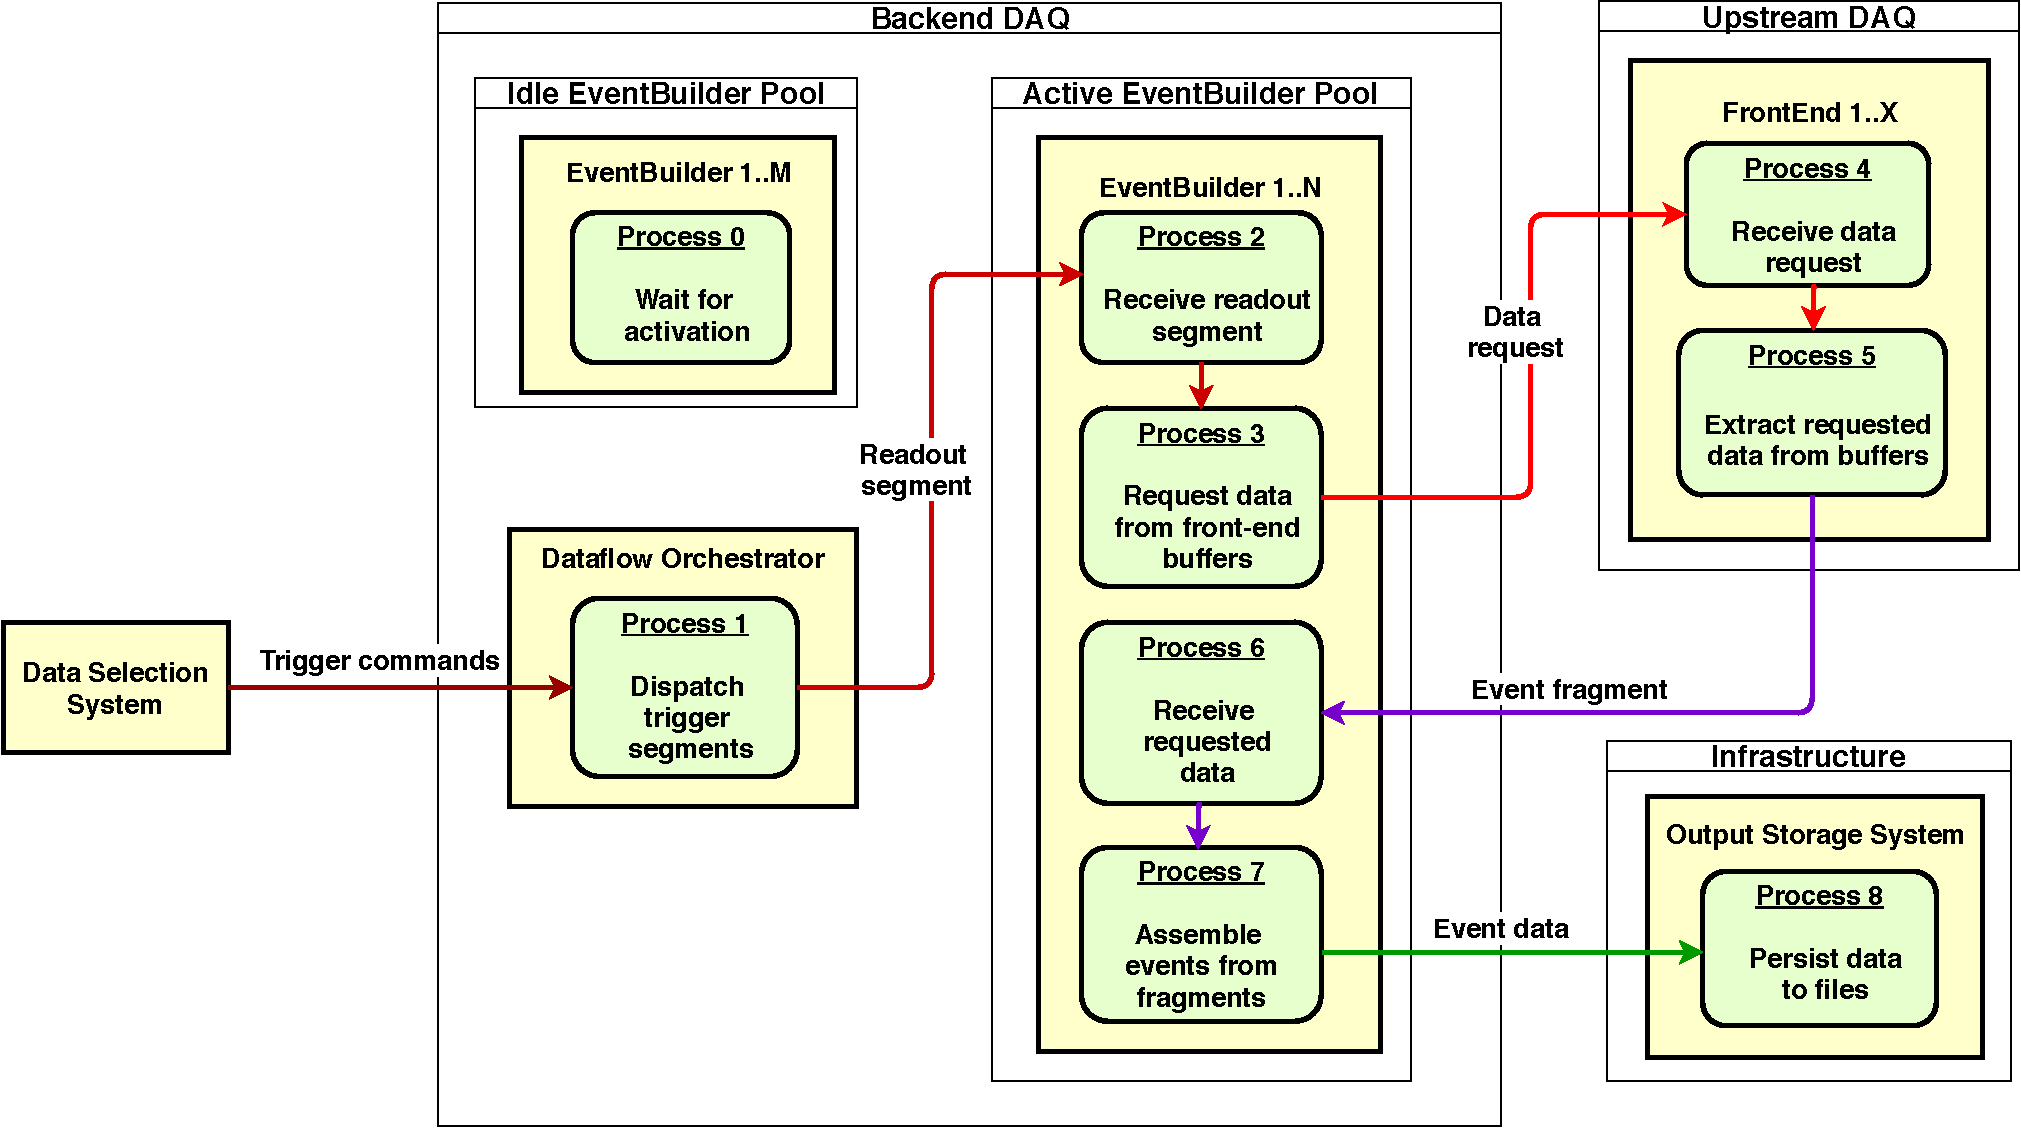
\includegraphics[width=\textwidth]{daq-backend.pdf}
\end{dunefigure}

\begin{itemize}
\item \dword{daqdfo} accepts a stream of \dwords{trigcommand} and dispatches each to an available \dword{eb} process as described in Section~\ref{sec:fd-daq:design-event-builder} for execution.
\item In atypical situations in which there are insufficient event builder resources available to handle the rate of triggers produced by the data selection sub-system, the DFO will alert the DS sub-system that the rate of triggers needs to be reduced.  When such reductions are requested, the \dword{daqdss} will update the calculation of the module-level \dword{daq} livetime appropriately.
\item The DFO will provide relevant data flow status and statistics information to the monitoring processes that are described in Section~\ref{sec:daq:design:ccm:monitoring}. Given its central role and knowledge of the state of available event builder buffers, it will be able to provide important information about the health and performance of the system.
\end{itemize}

\subsubsection{Event Builder}
\label{sec:fd-daq:design-event-builder}

The \dword{daqbes} will provide the instances of the \dfirst{eb} most likely as
\dword{artdaq}~\cite{artdaq} components of the same name. 
As described above, each EB instance will

\begin{itemize}
  \item Receive a readout segment for execution. Execution entails interpreting the \dword{trigcommand} segment and querying the appropriate upstream \dword{daq} units to request data from the period of time. 
  \item Requests and their replies may be sent synchronously, and replies are expected even if data has already been purged from the upstream \dword{daq} units. (In that case, and empty fragment will be generated with appropriate error flags set).
  \item The received data then processed and aggregated, is finally saved to one or more files on the output storage system before it is transferred offline.
\end{itemize}

%%The final output files shall use data schema and file formats as described in Section~\ref{sec:fd-daq:design-data-model}.

As part of this, the EB sub-system will provide book-keeping functionality for the raw data.  This will include the documentating of simple mappings, such as which trigger is stored in which raw data file, as well as more sophisticated quality checks. For example, it will know which time windows and geographic regions of the detector are requested for each trigger, and in the unlikely event that some fraction of the requested detector data can not be stored in the event record, it will document that mismatch.

\subsubsection{Output Buffer}

The output buffer system is composed by the physical harware resource to host the incoming data and by the software services handling the final processing stages through the High-Level Filter and the transfer off-site to permanent storage.

It has two primary purposes.  First, it decouples the production of data from filtering and the
transfer of filtered data offline. It provides the elasticity needed by the \dword{daq} to deal with
perturbations in the flow of data, therefore minimizing the impact of temporary loss in filtering
performance due to hardware or software issues. Second, it provides local storage sufficient for
uninterrupted \dword{daq} operation in the unlikely event that the network connection between the
\dword{fd} and \fnal is lost.  A capacity of at least a few \si{\peta\byte} is envisioned,
sufficient to buffer the nominal output of the entire \dword{fd} for about one week even in the case of SNB events. Based on prior experience of the consortium with unusual losses of  connectivity at
other far detector experiment sites, this is a conservative storage capacity value.

The output buffer system will provide the relevant data flow status and statistics information to the monitoring processes that are described in Section~\ref{sec:daq:design:ccm:monitoring}. The knowledge of the health and performace of the of the buffer system will enable the monitoring system to promtly identify and address developing faults before they can have an impact on data taking.


\subsubsection{Data Network}
Upstream \dword{daq}, \dword{daqdss} and \dword{daqbes} \dword{daq} are interconnected by a \SI{10/100}{ Gbps} ethernet network for data exchange.
In particular the upstream \dword{daq} and \dword{daqdss} servers are connected through redundant \SI{10}{ Gbps} links to top-of-rack switches with \SI{10}{Gbps} uplinks.
The \dword{eb} and Output buffer hardware will support \SI{100}{Gbps} directly.
The \dword{daq} data network is connected to the \fnal network via a WAN interface.

\subsubsection{Data Model}
\label{sec:fd-daq:design-data-model}

The data model for the DUNE far detector describes the format and characteristics of the triggered data at each stage in the analysis chain, the grouping of the data into logical units such as runs, and the characteristics of ancillary data such as detector configuration parameters and calibration results.

The requirements that these place on the \dword{daq} are primarily in the areas of flexibility and traceability.  The \dword{daq} will have the flexibility to handle the readout of triggers that have a time window that is on the order of a single TPC drift time (for example a trigger associated with a beam gate window), triggers that have a time window of many seconds (such as for a supernova burst trigger), and windows between those two extremes (for detector and electronics studies).  In the area of traceability, the \dword{daq} system will provide the necessary level of detail regarding the conditions that triggered each event, the expected and actual regions of the detector that contributed raw data to each event, the conditions of the detector and electronics during data taking, the version and configuration of the software components used in the \dword{daq} chain, etc.

\subsection{Control, Configuration, and Monitoring}
\label{sec:fd-daq:design-run-control}

The \dfirst{daqccm}, illustrated in Figure~\ref{fig:daq-ccm-subsys}, consist of the software
subsystems to control, configure, and monitor the \dword{daq} system, as well as the detector components
participating to datataking. It provides a central access point for the highly distributed \dword{daq}
components, allowing them to be treated and managed as a single, coherent system, though their
corresponding subsystem interfaces. It is responsible for error handling and recovery, which is
achieved by designing a robust and autonomous fault-tolerant control system. The main goal is to
maximize system up-time, data-taking efficiency and data quality when the system faces programmatic
(i.e. calibrations) and unforeseen (hardware failures or software faults) change of data-taking
conditions. The \dfirst{daqccm} provides an access point, which is delegating user's actions to the
corresponding interfaces. The detector components and infrastructure elements access the \dfirst{daqccm}
subsystems through their provided interfaces. 

\begin{dunefigure}[DAQ CCM subsystem interaction]{fig:daq-ccm-subsys}{Main interaction among the three \dword{daqccm} subsystems.}
  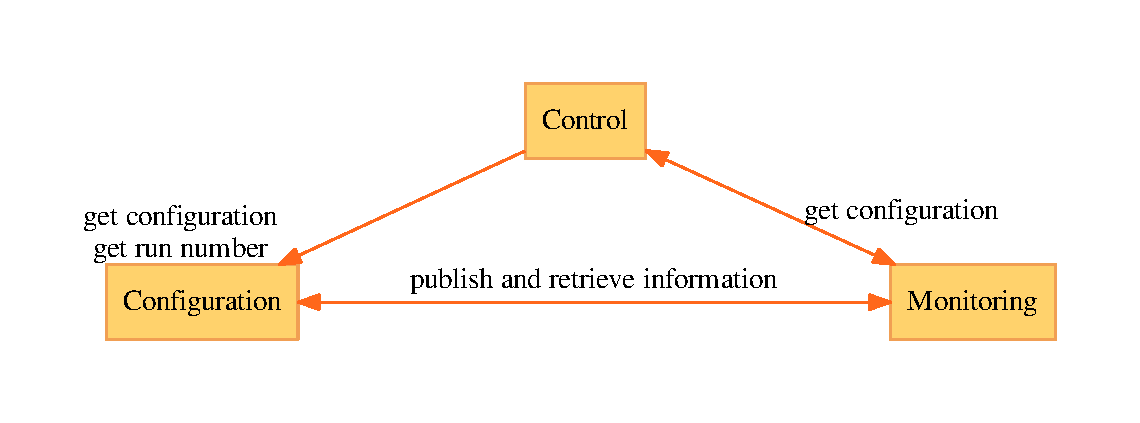
\includegraphics[width=0.9\textwidth]{daq-ccm-subsys.pdf}
\end{dunefigure}

The following sections describe each \dfirst{daqccm} subsystem, covering internal functions and dependencies between each other.

\subsubsection{Access}
\label{sec:daq:design:ccm:access}
Actions are defined as any kind of human interaction with the \dfirst{daqccm}. The access subsystem is responsible for the action delegation to internal function calls and procedures. It's implementation is driven by the control, configuration and monitoring interface specifications, and protects the direct access to detector and infrastructural resources. It also controls authentication and authorization, which locks different functionalities to certain actor groups and subsystems. As an example, only the detector experts can modify frontend configuration through the configuration interfaces, or only an expert user can exclude an APA's readout from data taking. 


\subsubsection{Control}
\label{sec:daq:design:ccm:control}

The control subsystem consists of several components and utilities, and also has additional subsystems to carry out dedicated roles. It enforces the implementation of required interfaces and actively manages \dword{daq} process lifetimes. It operates in a distributed, fault-tolerant manner due to protocols that will drive the FSM for state sharing. 

\begin{dunefigure}[DAQ control subsystem roles and services]{fig:daq-ccm-control}{Roles and services that compose the \dword{daq} control subsystem.}
  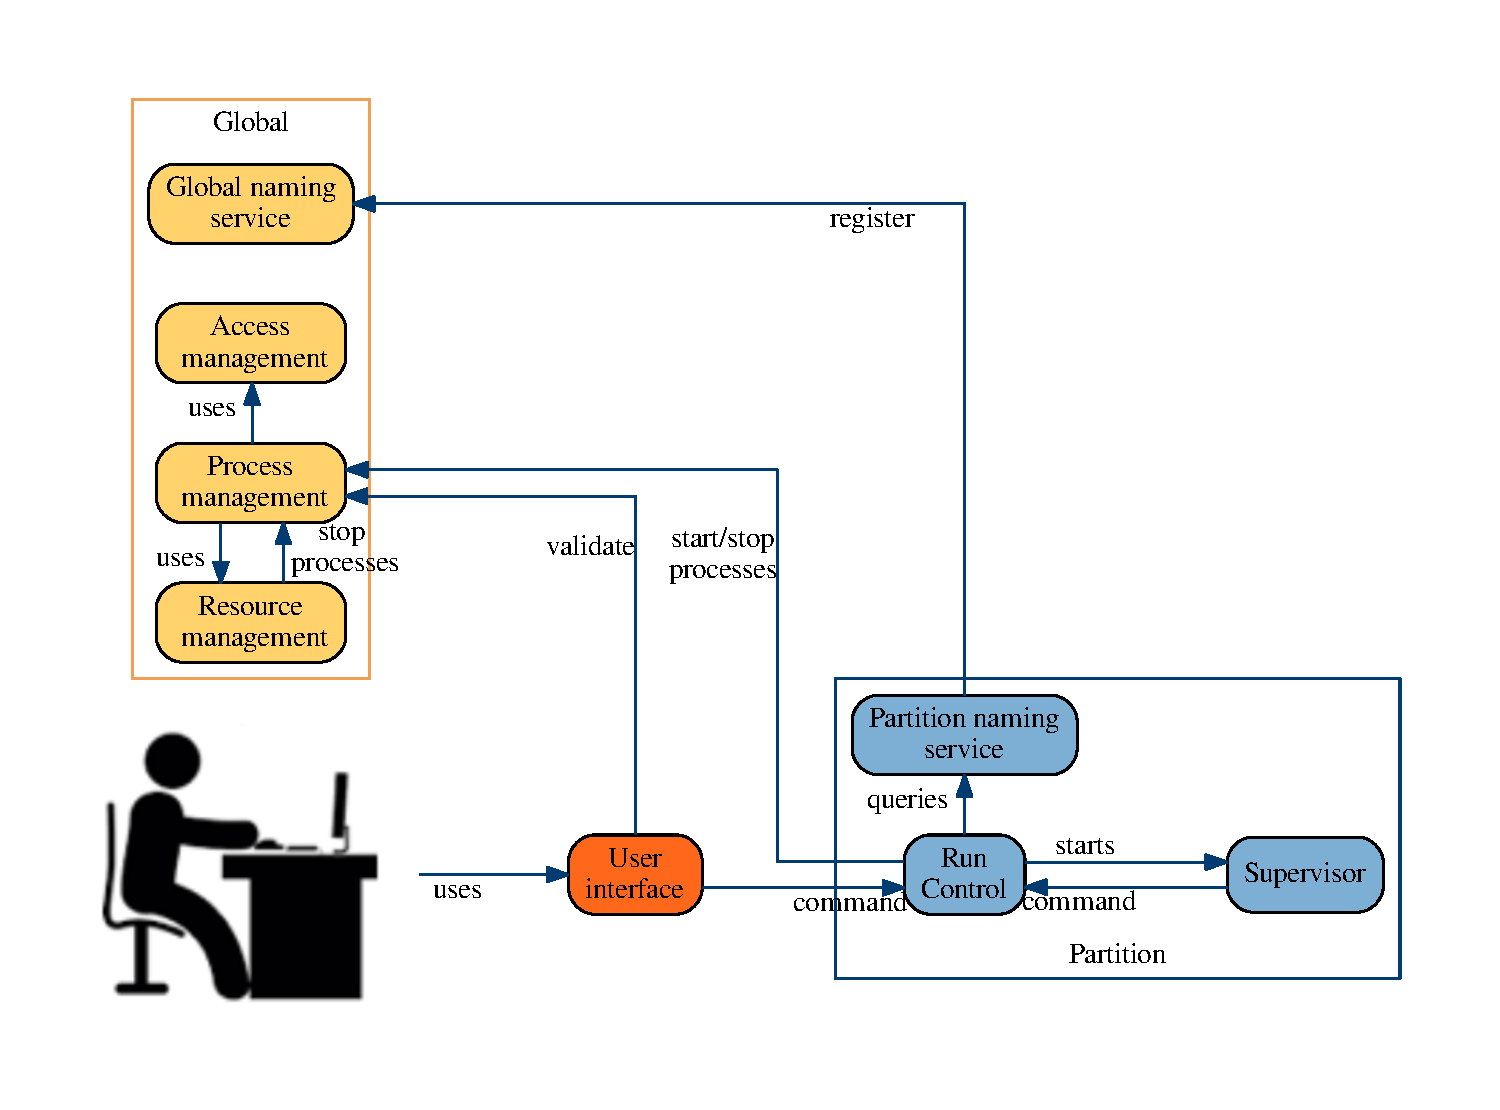
\includegraphics[width=0.8\textwidth]{daq-ccm-control.pdf}
\end{dunefigure}

It contains the following core components:
\begin{itemize}
\item Supervision System - It is responsible for manual and automated control and supervision of \dword{daq} components at any given time. In autonomous mode, the system makes attempts for fault-recovery, failover to backup instances of subsystems, and isolation of problematic regions of the control tree. This is carried out by a hierarchical rule-based planning or fuzzy logic system.
\item \dword{daq} Application - The CCM provides interfaces in order to communicate with processes of the \dword{daq}, and the ability to control and communication with the CCM. The Inter Process Communication (IPC) supports a mechanism to interact with all actors participating to data taking. The Finite State Machine (FSM) enforces the possible states and transitions that are specific to the experiment's components, and also describes them in a uniform way.
\item Run Control - This part of the control subsystem coherently steers the data taking operations. It interacts with all actors participating to data taking in a given partition. It consists of a hierarchical control tree, which can subdivide the \dword{daq} components into separated regions that may be acted upon independently.
\item Resource Management - Provides a global scope of available resources for the \dword{daq} components. This includes the mapping between the detector front-end readout units, processes, servers where they are spawned and required resources for the processes.
\item Process Management - It is responsible to manage process lifetime.
\end{itemize}

\subsubsection{Configuration}
\label{sec:daq:design:ccm:configuration}

The configuration subsystem provides several key elements for the configuration management of \dword{daq} components and detector front-end electronics. It provides a description of system configurations, the ability to define and modify configurations, and graphical user interfaces for the human user to access the data. Data access libraries will hide the technology used for the databases implementation. The subsystem is also responsible for the serialization, persistency, and bookkeeping of configurations. 

\begin{dunefigure}[DAQ CCM subsystem interaction]{fig:daq-ccm-config}{Main components of the \dword{daqccm} configuration subsystem.}
  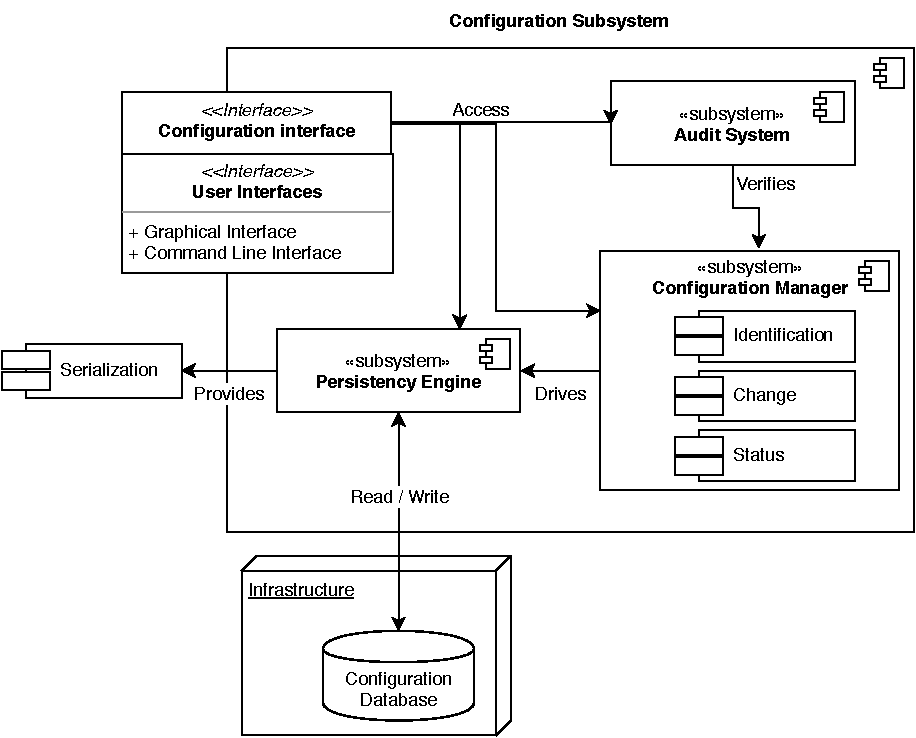
\includegraphics[width=0.8\textwidth]{daq-ccm-config.pdf}
\end{dunefigure}

The main components of the configuration subsystem are the following:
\begin{itemize}
\item Configuration Manager - It consists of the three main components of configuration management systems. The Identification Engine is a set of functionalities that are responsible for the definition of \dword{daq} components and their corresponding configuration specification. The Change Manager is responsible for providing control over altering the configuration specifications of components. The Status Engine is providing status and information about configuration specifications of individual, or set of \dword{daq} elements.
\item Audit System - This important subsystem is supporting the experts and decision making systems to verify the consistency of configuration specifications against the \dword{daq} and detector components. It provides results on mis-configurations and potential problems on configuration alignment and dependencies between components.
\item Persistency Engine - This component provides a single and uniform serialization module, which is strictly followed by every \dword{daq} component. Also responsible for configuration schema evolution and communication with the configuration database. The storage engine privileges will be only read and write operations, not allowing updates and removal of configurations. It also provides a redundant session layer for high-availability and load distribution.
\end{itemize}

The configuration system will mainly consist of standard configuration management components, with a high emphasis on the audit system, in order to verify that the global configuration of the \dword{daqccm} complies with the detector, physics and operational requirements.

\subsubsection{Monitoring}
\label{sec:daq:design:ccm:monitoring}

\begin{dunefigure}[DAQ monitoring subsystem roles and services]{fig:daq-ccm-monitoring}{Roles and services that compose the \dword{daq} monitoring subsystem.}
  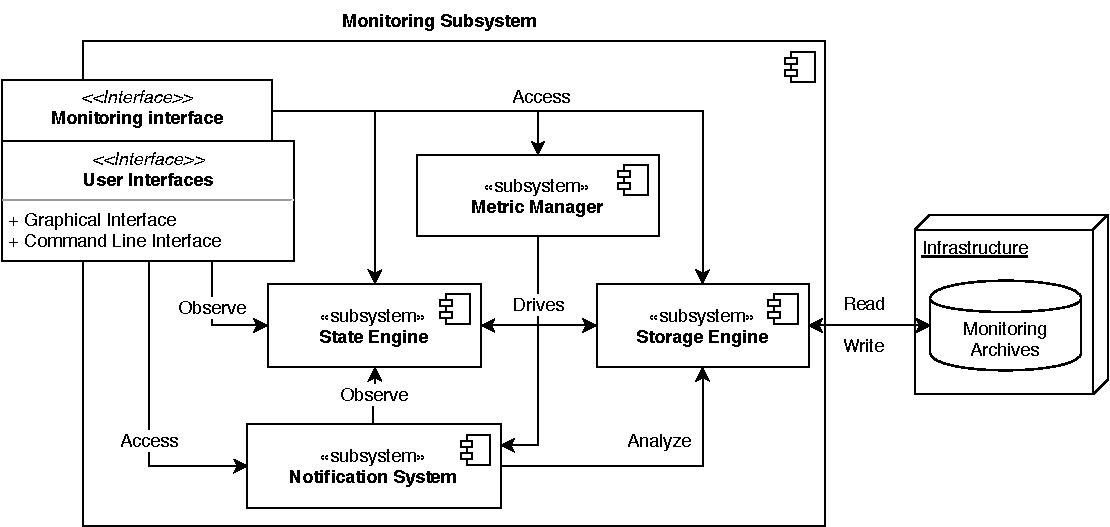
\includegraphics[width=0.8\textwidth]{daq-ccm-monitoring.pdf}
\end{dunefigure}

Highly-scalable and efficient operational monitoring is essential during data-taking periods. Any malfunctioning component of the experiment must be identified and reported as soon as possible. Therefore, the aim of the monitoring subsystem is probing and notifying the status of \dword{daqccm} components, services, and resources. There is also a requirement of \dword{daqccm} infrastructure monitoring and log aggregation. The types of monitoring information vary greatly depending on operational complexity, which require flexibility from the monitoring infrastructure for seamless additions, modifications and aggregated view on service degradation.
It consists of the following main components, also shown in Figure~\ref{fig:daq-ccm-monitoring}:


\begin{itemize}
  \item Metric Manager - It is responsible for the registration of metric data streams and corresponding aggregator functions. This central element is the collection of features and services that provides support for configurable operational monitoring of \dword{daqccm} services. \dword{daqccm} components and services that are registered via the Metric Manager, are reporting monitoring data to the State and the Storage Engines in a publish-subscribe fashion. 
  \item State Engine - This engine is responsible for providing the global state of the system at the current time. It subscribes to a set of registered metrics in the Metric Manager, and records the actual global state of the set for decision making systems (supervision, notification, and visualization).
  \item Storage Engine - Metrics may have different persistency requirements, for which the engine is responsible to archive the data with the settings of interval, smoothing, etc. It also provides an implementation for the most common communication protocols for the database backends (SQL, REST, etc.).
  \item Notification System - It is a rule-based system of scheduled and aimed notifications that occur in the case of state combinations. It defines soft and hard states of events and grace periods of alarms.
  \item User Interfaces - Provides graphical and command line user interfaces for monitoring configuration management and visualization of metric data.
\end{itemize}

Monitoring being a key requirement in the industry for computer clusters and their applications, the proposed solution is the adaptation of mature, robust, and open-source third party tools, with the extension of DUNE \dword{daqccm} specific interface implementations and configurations of these monitoring systems. 


\subsubsection{Inter-Process Communication}
\label{sec:daq:design-ipc}

The DUNE FD \dword{daq} is an asynchronous, parallel distributed data processing system. 
It is composed of many independent processes which ingest and produce messages. 
The mechanisms of such message passing are generally called \dword{ipc}. 
Referring to Figure~\ref{fig:fd-daq:layout}, \dword{ipc} is used for both in-band detector data flow between upstream \dword{daq} and back-end \dwords{eb} and for out-of-band messages as part of \dword{daqccm}.  The \dword{ipc} used by the \dword{daqdss} spans both descriptions as it passes derivations of a subset of detector data (trigger primitives, candidates) and culminates in a source of out-of-band message (\dwords{trigcommand}) to direct the readout by \dword{eb} and other components of detector data that is held in the upstream \dword{daq} buffers.

The ZeroMQ~\cite{zeromq} smart socket library is 
the basis of a system being developed and evaluated for parts of both in-band and out-of-band \dword{ipc}. 
As part of the \dword{daqccm}, this includes the issuing of control and reconfiguration commands to and receiving of monitoring messages from essentially all \dword{daq} components. 
As part of \dword{daqdss}, this includes the transfer of \dword{trigprimitive}, candidate and command messages. 
In the upstream \dword{daq} this includes the \dfirst{daqubi} that  provides access to the upstream \dword{daq} primary buffers for queries by \dword{eb} and other components. 
\dword{ipc}  must be implemented broadly across many \dword{daq} systems and ZeroMQ allows their problems to be solved in common, shared software.  As \dword{daqccm} has the most complex \dword{ipc}  needs, this work is organizationally considered part of this system.

% One ZeroMQ facility in particular is worth additional description. 
% Zyre\footnote{An open source framework for proximity-based peer-to-peer applications. \url{https://github.com/zeromq/zyre}.} 
% will provide a decentralized implementation \dword{daqdispre} (see Section~\ref{sec:daq:design:ccm:control}). 
% It uses \dword{udp} broadcast beacons and a connected followup to provide peer discovery on the local network. 
% A heartbeat mechanism provides presence so that a component may discover when a peer has become unresponsive.  
% As Zyre uses the network itself, there is no central point of failure. 
% The network provides the naming service described above. 
% Zyre also allows for more centralized, connection oriented, discovery which can be used to allow the process to span networks.

As described in~\ref{sec:fd-daq:design-backend}, \dword{artdaq}~\cite{artdaq} utilizes \dword{ipc}  between its back-end components. 
It has been well tested with \dword{protodune} and other experiments. 
\dword{artdaq} may be used for some portions of the \dword{ipc}  described above. 
For example, if the \dword{daqubi} is implemented as an \dword{artdaq} Board Reader it would necessarily use \dword{artdaq} \dword{ipc} . 
This would limit the types of clients that could query for data in the buffers to be \dword{artdaq} modules. 
Understanding how to optimally select an \dword{ipc}  for such parts of the \dword{daq} connection graph is an area of ongoing R\&D effort.

\subsubsection{Hardware}
\label{sec:daq:design:ccm:hardware}

The \dword{daqccm} software suite will run on approximately 15 servers interconnected by a \SI{1}{Gbps} ethernet network to upstream \dword{daq}, \dword{daqdss}, \dword{daqbes} as well as detector and calibration daq interface elements. While this network has a lower throughput compared to the data network, it has many more endpoints O(2000).

\subsection{Data Quality Monitoring}
\label{sec:fd-daq:design-data-quality}

While the \dword{daqccm} contains an element of monitoring (Section~\ref{sec:daq:design:ccm:monitoring}), here \dfirst{dqm} refers to a subsystem that quickly analyzes the data in order to determine the general quality of the detector and \dword{daq} operation.
This is in order to allow operators to promptly detect and respond to any unexpected changes and assure high exposure times for later physics analyses. 
A \dword{daq} \dfirst{dqm} 
will be developed (including necessary infrastructure, visualization,
and algorithms), which will process a subset of detector data in order
to provide prompt feedback to the detector operators. 
This system will be designed to allow it to evolve as the detector and its data is understood during commissioning and early operation and to cope with any evolution of detector conditions.


\subsection{Timing and Synchronization}
\label{sec:sp-daq:design-timing}

All components of the \dword{fd} use clocks derived from a single
\dfirst{gps} disciplined source, and all module components are
synchronized to a common \SI{62.5}{MHz} clock.
%
This rate is chosen in order for this common clock to satisfy the requirements of the detector electronics of both the single-phase and the dual-phase far detector modules.
%
To make full use of the information from the \dword{pds}, the common clock must be aligned within a single detector %unit 
module with an accuracy of \bigo{\SI{10}{\nano\second}}. 
For a common trigger for a \dword{snb} between modules, the timing must have an accuracy of order \SI{1}{\milli\second}.
However, a tighter constraint is the need to calibrate the common clock to universal time derived from \dword{gps} so the \dword{daqdsn} algorithm can be adjusted inside an accelerator spill, which again requires an absolute accuracy of order \SI{1}{\micro\second}. The design of the timing system allows for an order-of-magnitude better synchronization precision than these requirements, allowing a substantial margin of safety and the possibility for future upgrades to front-end electronics.

The \dword{dune} \dword{fd} uses a improved version of the \dword{protodune} timing
system, where a design principle is to transmit synchronization messages over
a serial data stream with the clock embedded in the data. The format
is described in \citedocdb{1651}. The timing system design is
described in detail in \citedocdb{11233}.

Central to the timing system are four types of signals:
\begin{itemize}
\item a \SI{10}{\mega\hertz} reference used to discipline a stable master clock,
\item a \dfirst{pps} from the GPS,
\item a \dword{ptproto} signal providing an absolute time for each \dword{pps}, and
\item an \dfirst{irig} time code signal
  used to set the timing system 64-bit time stamp.
\end{itemize}

The timing system synchronization codes are distributed to the \dword{daq} readout components in the \dfirst{cuc} and the readout components on the cryostat via single mode fibers and passive splitters/combiners.
All custom electronic components of the timing system are contained in two \dword{utca} shelves; at any time, one is active while the other serves as a hot spare.
The \SI{10}{MHz} reference clock and the \dword{pps} signal are received through a single-width \dword{amc} at the center of the \dword{utca} shelf.
This master timing \dword{amc} is a custom board and produces the timing system signals, encoding them onto a serial data stream.
This serial data stream is distributed over a backplane to a number of fanout \dwords{amc}.
The fanout \dword{amc} is an off-the-shelf board with two custom \dwords{fmc}.
Each \dword{fmc} has four \dword{sfp} cages where fibers connect the timing system to each detector component (e.g., \dword{apa}) or where direct attach cables connect to other systems in the \dword{cuc}.

To provide redundancy, two independent GPS systems are used,
one with an antenna at the surface at the Ross shaft, and the other
with an antenna at the surface at the Yates shaft. Signals from either
GPS are fed through single-mode optical fibers to the \dword{cuc}, where
either GPS signal can act as a hot spare while the other is active. 
Differential delays between these two paths are resolved by a second pair of fibers, one running back from the timing system to each antenna, allowing closed-loop delay estimation.


\section{Design Validation and Development Plans}
\label{sec:fd-daq:validation}

The following strategy will be followed in order to validate and
develop the \dword{dune} \dword{fd} \dword{daq}:
\begin{itemize}
\item Use \dword{protodune} and other teststands as a basis for prototyping, development and validation
of the \dword{daq} design.
\item Use Monte Carlo simulations and emulations in order to augment actual hardware
demonstrations and validate triggering schemes in the FD environment.
\end{itemize}

% This strategy reflects the current \dword{daq} project schedule,
% provided in Section~\ref{sec:fd-daq:schedule}, which
% comprises several phases, including an intense development phase
% through 2020 that culminates in an engineering design
% review (EDR) in Q1 of 2021. At this milestone, the system design will be
% finalized and demonstrated to be capable of meeting the requirements of the
% final \dword{daq} system. After the development phase, a
% pre-production phase will begin and will end with a production readiness
% review (PRR). By then, final designs of all components
% will be complete.

The design and implementation of the \dword{daq} is being carried out using an iterative prototyping model, which is well suited for a system that largely relies on commercial off the shelf hardware components, on communication and information technologies that are rapidly evolving, and that mainly requires software and firmware development effort.
The advantage of the prototyping model is also that it facilitates the identification of and collaboration among experts from a large number of institutions, thanks to the focussed effort of achieving the short term objectives established through each prototyping iteration.

Once the identification of convenient technologies will have been completed and the overall system requirements will have been refined, the project will switch to an iterative incremental model, ensuring that, step-by-step, functional and performance requirements will be met by each of the sub-components individually and by the \dword{daq} system globally.
The overall schedule, summarised in Section~\ref{sec:fd-daq:schedule},
reflects the different development and production time scales that are
envisioned for the various \dword{DAQ} components.


The following subsections summarize past, ongoing, and planned
development and validation studies and identify how anticipated outcomes
will be used to finalize the \dword{daq} design.

\subsection{ProtoDUNE Test Beam}

\label{sec:fd-daq:protodune}

The \dword{fd} \dword{daq} consortium constructed and operated the \dword{daq} system~\cite{Sipos:2018auh} for \dword{protodune}, which included two parallel \dword{daq} readout architectures, one based on \dword{felix}, developed by ATLAS \cite{atlas-felix}, and the other on \dword{rce}, developed at SLAC. \dword{daq} design and construction for \dword{protodune} began in Q3 of 2016, and the system became operational at the start of the beam data run in Q4 of 2018. The detector is continuing to run at the time of writing, recording cosmic ray activity, and providing further input for \dword{daq} development toward \dword{dune}. 

Figure~\ref{fig:daq-protodune} depicts the \dword{protodune} \dword{daq} system. 
The \dword{daq} is split between the \dword{felix} and \dword{rce} implementations. The two architectures share the same back-end and timing and trigger systems. 
Neither of these tested architectures exclusively represents the baseline design for the DUNE \dword{fd}. Instead, each rouhgly maps onto one of two data processing approaches: one in which the data is processed exclusively in custom-designed \dword{fpga} firmware and carrier board, and the other in which the data is processed primarily with custom software run in commodity servers. The baseline design presented here merges elements of the two approaches. Specifically, it uses \dword{felix} as the hardware platform for data receiving and handling, and an co-processor FELIX daughter card (analogous to the \dword{rce} platform used at \dword{protodune}) to provide additional, dedicated data processing resources.


\begin{dunefigure}[ProtoDUNE DAQ system]{fig:daq-protodune}{The \dword{protodune} \dword{daq} system.}
  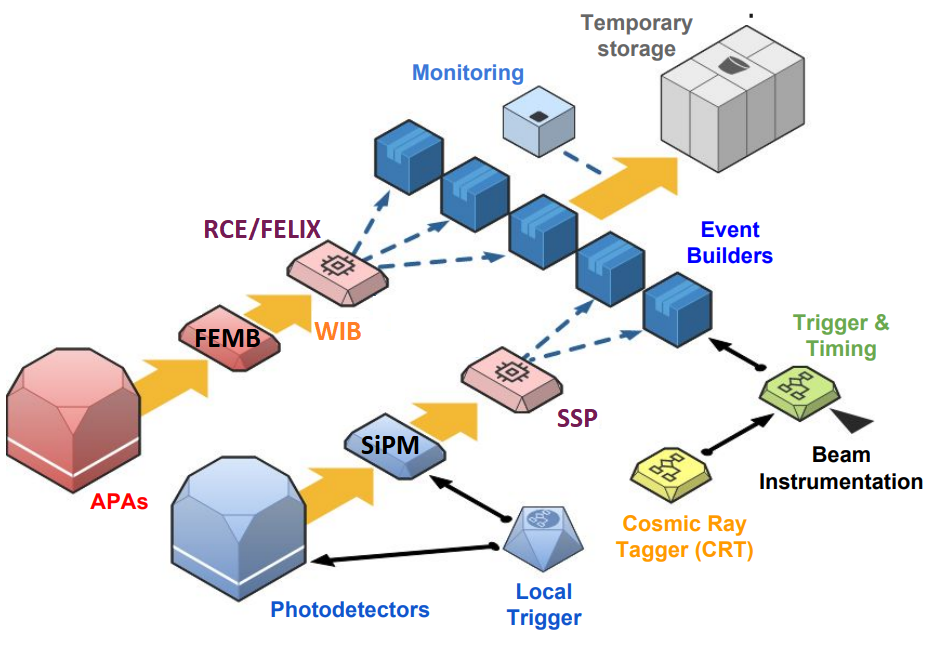
\includegraphics[width=0.8\textwidth]{daq-protodune-overview.png}
\end{dunefigure}

Besides overall readout architecture, the \dword{protodune} and \dword{dune} \dword{daq} systems exhibit two key differences. 
First, the \dword{protodune} \dword{daq} is externally triggered (and at a trigger rate over an order of magnitude higher than that anticipated for \dword{dune}). Because of this, the \dword{protodune} \dword{daq} does not facilitate online data processing from the \dword{tpc} or \dword{pd} systems for self-triggering. 
Second, the \dword{protodune} system sits at the surface with a much higher data occupancy due to cosmic ray activity.
Overcoming the first key difference in order to demonstrate \dword{daqdsn} capability for the \dword{fd} \dword{daq} design is a main component of future \dword{daq} development plans.

% Continuous self-tirggering of the detector is also new with respect to
% other ongoing or planned near-term \dword{lartpc} experiments, including
% MicroBooNE, SBND, and ICARUS. Both MicroBooNE and ICARUS have demonstrated
% self-triggering in coincidence with external gates, which effectively
% limits both data and trigger rates, and is not a viable solution for
% DUNE's off-beam physics program, as it would effectively limit
% exposure and therefore physics sensitivity. %On the other hand, ICARUS
% %has ...
% MicroBooNE has demonstrated successful continuous readout of a \dword{lartpc},
% via use of dynamic and fixed-baseline zero-supression implemented in
% firmware for both \dword{tpc} and \dword{pds} readout. SBND, which utilizes the same readout
% system as MicroBooNE, will investigate trigger primitive generation
% and self-triggering based on \dword{tpc} information in the timescale of 2021-2023.

\subsubsection{ProtoDUNE Outcomes}

The \dword{protodune} \dword{daq} supported a test-beam experiment, and the requirements of the DUNE \dword{daq} are substantially different in scale and performance.
However, the successful operation of the \dword{protodune} \dword{daq} has provided several key demonstrations for final system, in particular the data flow architecture, run configuration and control, and back-end functionality.

Specifically, \dword{protodune} has demonstrated: 
\begin{itemize}
\item Upstream \dword{daq}: front-end readout hardware and data flow functionality servicing two out of the six \dwords{apa} was successfully employed in \dword{protodune}.
  The data from each APA was continuously streamed to a single FELIX board hosted in a dedicated computer which then transferred it to two other computers for buffering and readout.
  The baseline upstream \dword{daq} for \dword{dune} FD will retain one APA per FELIX board but place two FELIX boards and the buffering and readout functionality all together in a single \dword{fec}. 
  In addition to data flow functionality, \dword{protodune} \dword{fe} readout also demonstrates the interface to the front-end TPC electronics, and scalability to DUNE. It also supports host server requirements and specifications. Finally, it serves as platform for further development involving co-processor implementation and data selection aspects.
\item \dword{daqbes}, \dword{daqccm} and software infrastructure:
 successful \dword{daqbes} implementation, including event builder
  farm and disk buffering, as well as an initial implementation of \dword{daqccm} functions. This has allowed the
  development and exercising of system partitioning, and provides a
  basis for scalability to DUNE. \dword{protodune} also serves as
  a platform for further system development, in particular in \dword{daqccm} and for the data flow orchestrator part of the
  \dword{daqbes}.
\item Data selection and timing: successful operation of the timing
  distribution system, and external trigger distribution to the
  front-end readout.
\end{itemize}

Besides demonstrating end-to-end data flow, an important outcome of
\dword{protodune} has been the delineation of cross-system
interfaces, i.e.~understanding the exact \dword{daq} scope and the interfaces to \dword{tpc}, \dword{pds}, and offline computing. The use of commodity solutions
where possible, and leverage of professional support from CERN IT 
substantially expedited the development and success of the project, as
did the strong on-site presence of experts from within the consortium during early installation and
commissioning. 
Outcomes specific to \dword{protodune} subsystems are discussed in
greater detail in~\cite{Hennessy:CDRReview}. 

\subsection{Ongoing Development}
\label{sec:sp-daq:design-validation}

Subsystem development is ongoing at \dword{protodune} at the time of
writing. A detailed schedule for 2019 is available
in \cite{bib:docdb14095}. Major development plan milestones are:
\begin{itemize}
\item optimization and tuning of the \dword{fe} readout
\item optimization and tuning of the \dword{artdaq} based dataflow software
\item enhancement of monitoring and troubleshooting capabilities
\item introduction of CPU-based hit finding (necessary for \dword{pds} readout)
\item introduction of \dword{fpga}-based hit finding (for \dword{tpc} readout)
\item implementation of online software data selection beyond trigger
primitive stage (introduction of trigger candidate generation, and
\dword{trigcommand} generation), and tests on well identified interaction
topologies (e.g. long horizontal tracks, or Michel electrons from muon decay)
\item integration of online \dword{trigcommand} and modified data flow to event
builder to facilitate self-triggering of detector
\item implementation of extended \dword{fpga}-based front-end functionality
(e.g., compression)
\item prototyping of fake \dword{snb} data flow in \dword{fe} and back-end.
\end{itemize}

Below, we focus on ongoing developments related to upstream \dword{daq},
data selection, and \dword{daqccm} prototyping, which is relevant to all \dword{daq} subsystems. These are the key areas where new technologies, beyond \dword{protodune}, remain to be designed and tested.


\subsubsection{Upstream DAQ Development}

%The detector readout for DUNE will be based Front-End Link EXchange (FELIX)[?] system, originally developed for the ATLAS experiment DAQ upgrades.
The use of \dword{felix} as the front-end readout technology for DUNE was
successfully prototyped at \dword{protodune}, initially for the readout of one
\dword{apa}. In \dword{protodune}, \dword{felix} allows streaming of data arriving o- multiple 10
Gbps optical point-to-point links into commercial host memory and,
from there, storing, dispatching or processing of the data via
software. 

In \dword{protodune}, a single \dword{apa} \dword{felix}-based readout consists of two servers with a point-to-point 100 Gbps network connection to the \dword{felix} host computer.
The \dword{felix} I/O card interfaces with its host PC through 16-lane PCIe 3.0 (theoretical bandwidth of \SI{16}{GB/s}).
It transfers the incoming WIB data directly into the host PC memory using continuous DMA transfer. The \dword{felix} host PC runs a software process that publishes the data to any client subscribing to it.
Subscriptions may identify from which input optical links the received data stream will be sourced.
The clients consuming these streams are ``BoardReader'' processes implemented in the \dword{artdaq} data acquisition toolkit.
In order to sustain the data rate, modest modifications of the firmware and software were carried out specifically for \dword{protodune}: each \dword{felix} host receives and publishes data at $\sim$75 Gbps. The BoardReader hosts are equipped with embedded Intel QuickAssist (QAT)~\footnote{Intel\textregistered QuickAssist Technology, \url{https://www.intel.com/content/www/us/en/architecture-and-technology/intel-quick-assist-technology-overview.html}.} technology for hardware accelerated data compression. The \dword{protodune} application of the \dword{felix} \dword{fe} readout is shown in Figure~\ref{fig:sp-daq:felix-pd-impl}.


In DUNE only a very small fraction of the data received via the \dword{felix}
system will ever need to leave the host: thus it is not required to
implement very high speed networked data dispatching. On the other
hand it may be interesting to carry out data processing and buffering
on the host. While this is not the baseline design for DUNE, R\&D is
ongoing at \dword{pdsp} to evaluate the feasibility of
implementing hit finding, data buffering, and possibly even local
\dwords{trigcandidate} generation on the \dword{felix} host. 


\begin{dunefigure}[Topology of the FELIX-based
    upstream DAQ of ProtoDUNE]{fig:sp-daq:felix-pd-impl}{The topology of the \dword{felix}-based
    upstream \dword{daq} of \dword{protodune} (from~\cite{pdsp-felix}). The \dword{felix} host servers are publishing the data from the \dwords{wib} over \SI{100}{Gb\per\second} network interfaces. The BoardReader hosts are carrying out trigger matching, data compression and forwarding of fragments to the event builder.}
  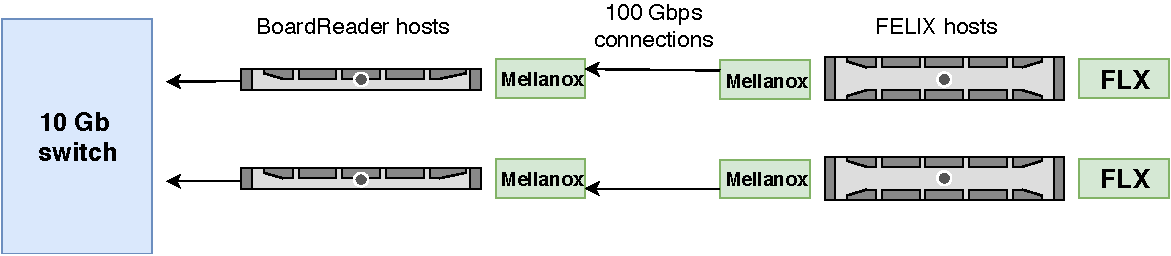
\includegraphics[width=0.9\textwidth]{daq-protodune-server-topology-2x2.pdf}
\end{dunefigure}

The \dword{daq} team is investing substantial effort into the introduction of
a triggering chain based on the \dword{tpc} data into \dword{protodune}, which will
allow to carry out pre-design prototyping studies of the complete flow
of data of the DUNE \dword{daq}.  
The \dword{felix}-based readout system will be adapted to support the
different studies, from co-processor based data handling in firmware
(including trigger primitive generation, compression, and buffering) to software-based processing, on a single
server. Benchmarking and optimization of the \dword{felix} firmware and
software will also continue, with the aim of further compacting the
readout by supporting two \dwords{apa} on a single server. 

\subsubsection{Co-processor Development}


Upstream \dword{daq} development efforts at \dword{protodune} include a parallel test platform for trigger primitive generation, compression, and buffering firmware validation for the \dword{fpga} co-processor board. The platform for these tests will initially be a Xilinx ZCU102 development board. Passive optical splitters will be inserted into the fiber path downstream of the WIBs, providing duplicate data inputs for the test hardware, without disrupting the main readout path of \dword{protodune}. Tests using the development board will first focus on generation of trigger primitives, which will be read out over the network via IPBus\cite{Larrea:2015wra}. The ZCU102 includes 512MBytes of DDR4 RAM connected to the \dword{fpga} programmable logic, as well as a four lane PCIe Gen 2 socket which will host an \dword{nvme} SSD on an adapter. This combination of hardware will allow tests of buffering and compression of readout data, in parallel with trigger primitive generation. The ZCU102 will subsequently be replaced with a ``\dword{felix} demonstrator'' using a Xilinx Virtex-7 Ultrascale+ \dword{fpga}, connected to a custom \dword{fpga} co-processor board via an FMC+ connector. These boards represent the first prototypes for the final system hardware.

Tests using the development board will focus on functionality rather than data throughput. However, the tests will provide estimates of \dword{fpga} logic and memory resources that can be scaled up to the full system. Tests using the \dword{felix} Demonstrator and PBM at \dword{protodune} will focus on scaling the functional tests performed using the ZCU102 to a full demonstration of trigger and readout functionality for a full \dword{apa}. In addition, this platform will facilitate integration with the prototype \dword{daqdss} and \dword{daqbes} subsystems at \dword{protodune}. 

\subsubsection{Data Selection Development}

\begin{dunefigure}[CPU core-time for primitives and CPU utilization in live data]{fig:daq-cpu-hf-speed}{CPU core-time (left) required to find primitives in simulated signal and noise data across 960 collection channels.
    In this test, the data has been pre-formatted to facilitate the use of SIMD hardware accelerated functions (AVX2). 
    Per thread CPU utilization (right) to process live data from a \dword{protodune} \dword{apa}.
    Processing includes data reformatting, trigger primitive generation, and output message formation.
    Each thread, one per FELIX link, requires about 75\% CPU core utilization to keep up.
    Variation in utilization reflects the variations in levels of ionization and noise activity in the input data and is due to output message formation.
    The peak usage at the start arises from input buffering while the process is initializing. 
    Once operational state is achieved, this brief backlog is processed.}
  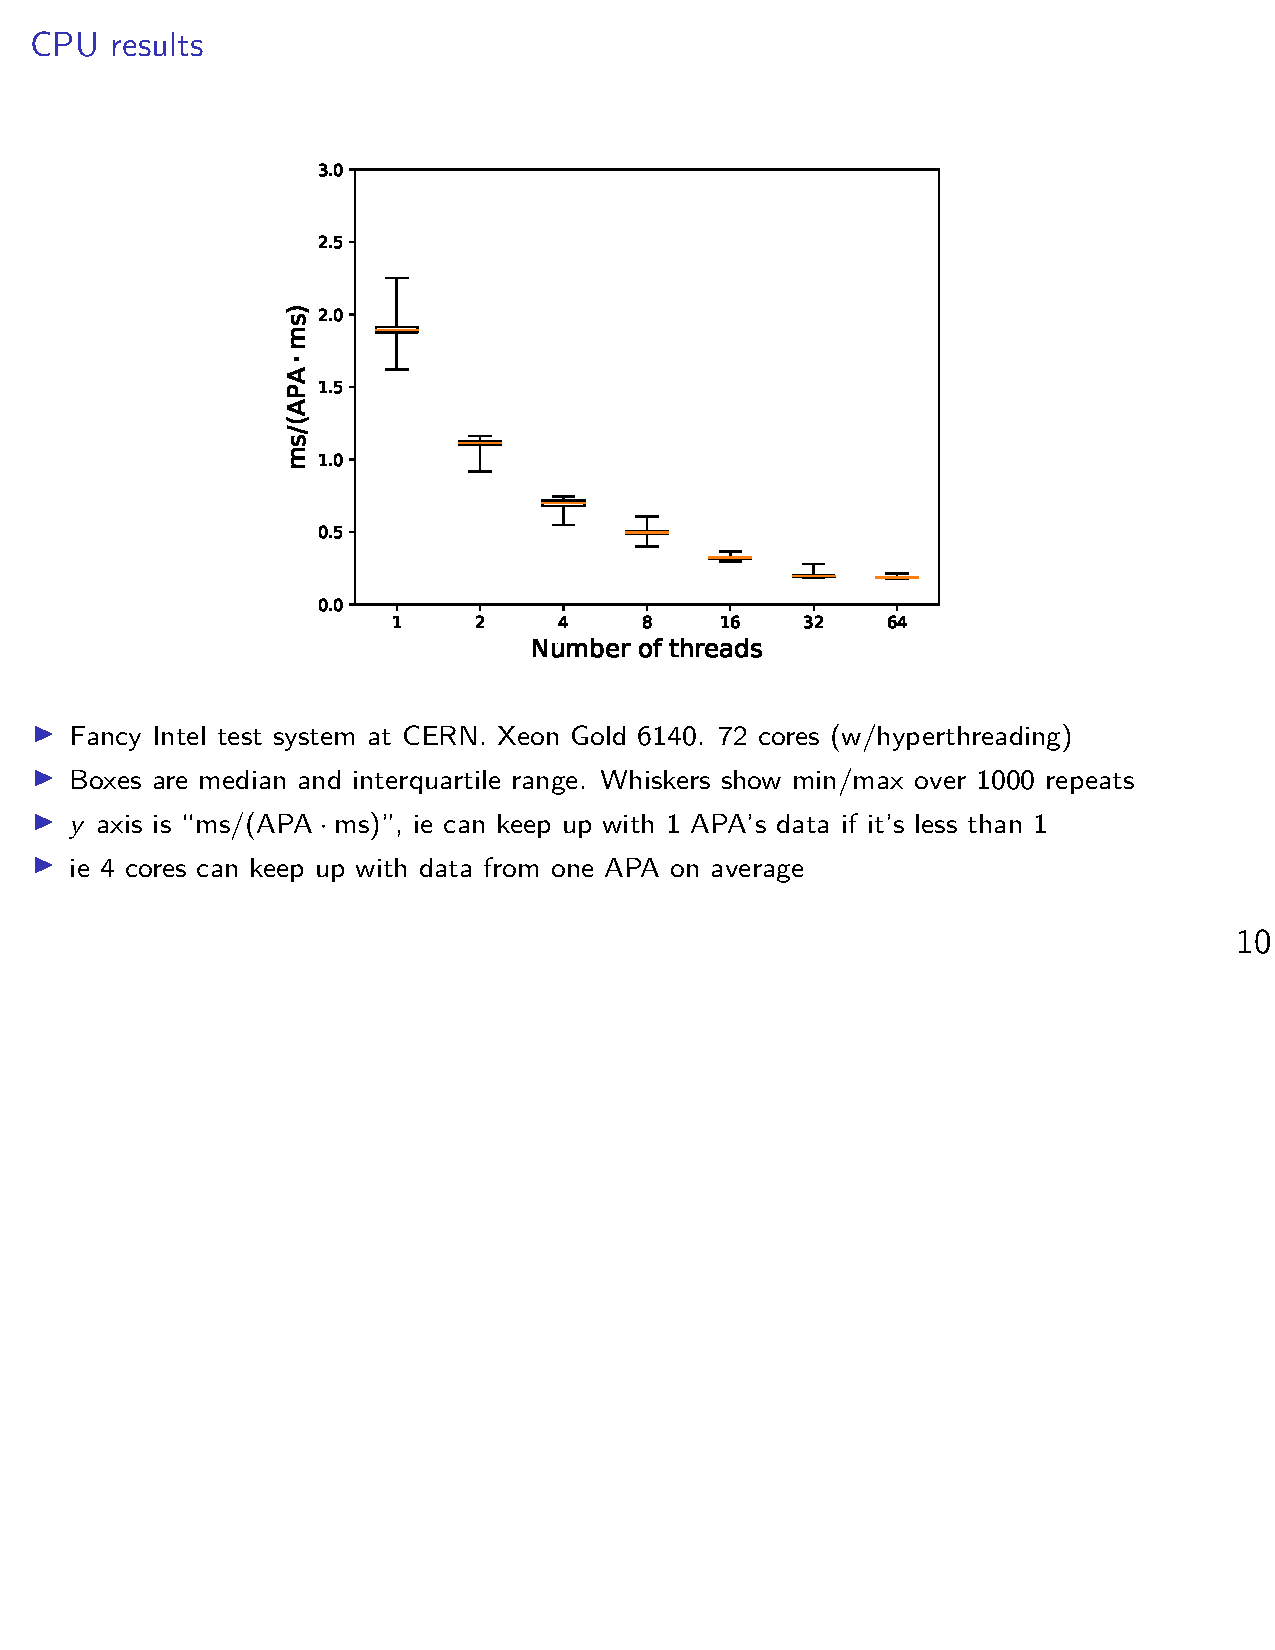
\includegraphics[height=6cm,clip,trim=4cm 16.5cm 4cm 2cm]{daq-primitive-cpu-speed.pdf}%
  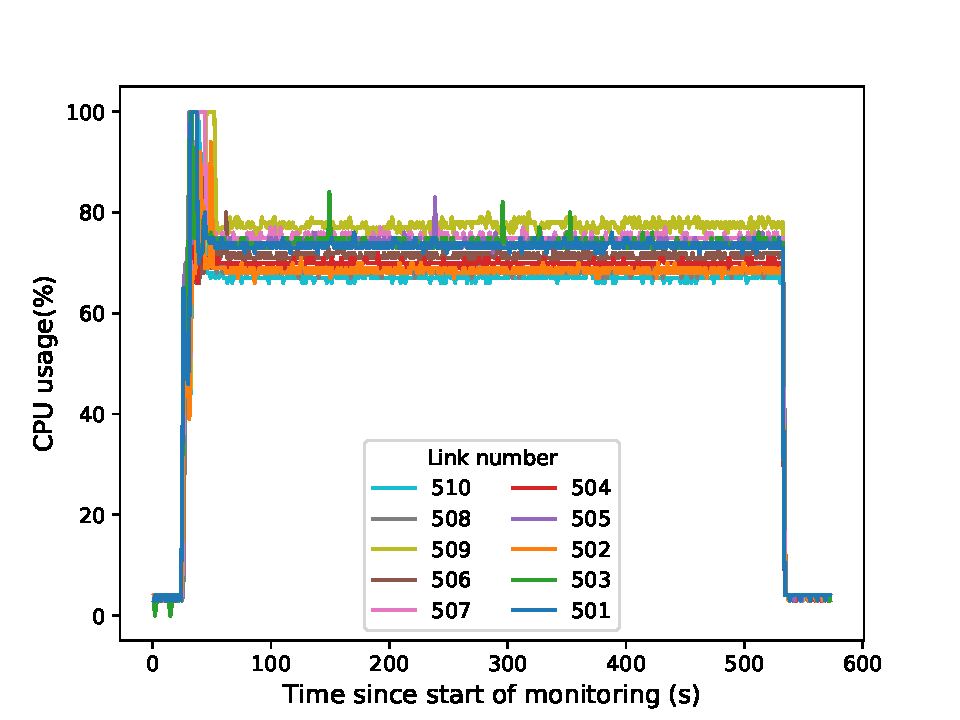
\includegraphics[height=6cm,clip,trim=0cm 0cm 0cm 5mm]{apa5-processing-ptmp-pinning-2019-06-10-run8219-for-tdr.pdf}
\end{dunefigure}

\begin{dunefigure}[Trigger primitives in ProtoDUNE-SP data]{fig:daq-hitfinder}{Example result of the trigger-primitive software (``hit finder'') applied to ADC waveform data spanning 96 collection channels that are sensitive to activity in the drift volume of \dword{pdsp}. 
    At left, the figure shows the ADC sample values relative to pedestal which are input to the algorithm. 
    At right, these same data are shown with a green $\times$ marking each trigger primitive found. 
    The inset is a zoomed region showing in detail the alignment of the input waveforms and the derived trigger primitives.
    In this test, the algorithm runs on the continuous stream of ADC waveforms prior to readout while actual readout was prompted by an external trigger.}
  % 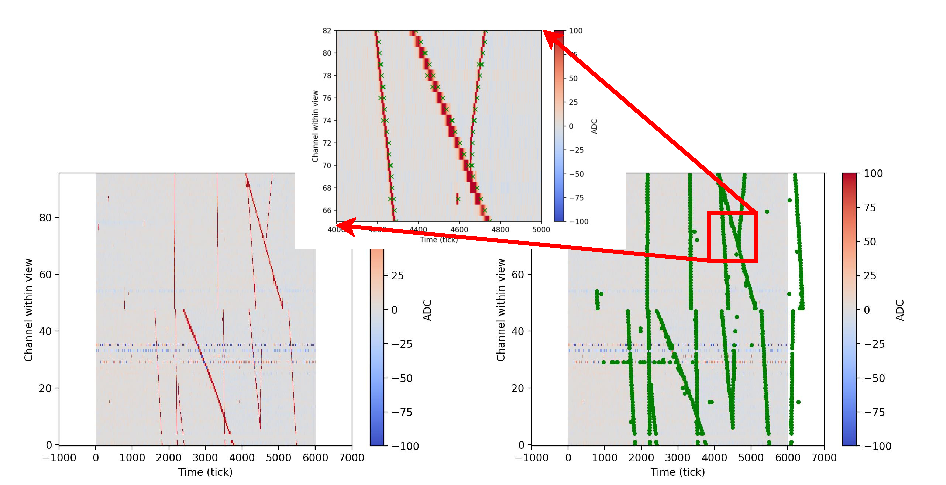
\includegraphics[width=0.9\textwidth]{daq-hitfinder-montage.pdf}
  \begin{tikzpicture}
    \node[inner sep=0] (raw) at (0,0) {
      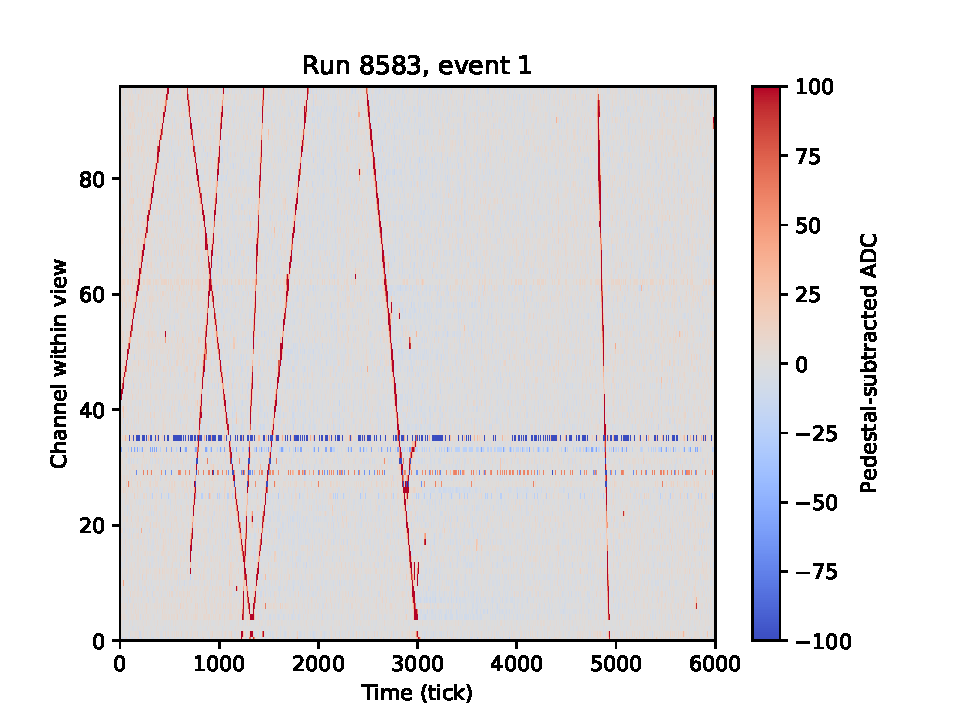
\includegraphics[height=7cm]{raw-event-96chans-run8583-evt1.pdf}
    };
    \node[inner sep=0, right = 0cm of raw] (hit) at (raw.east) {
      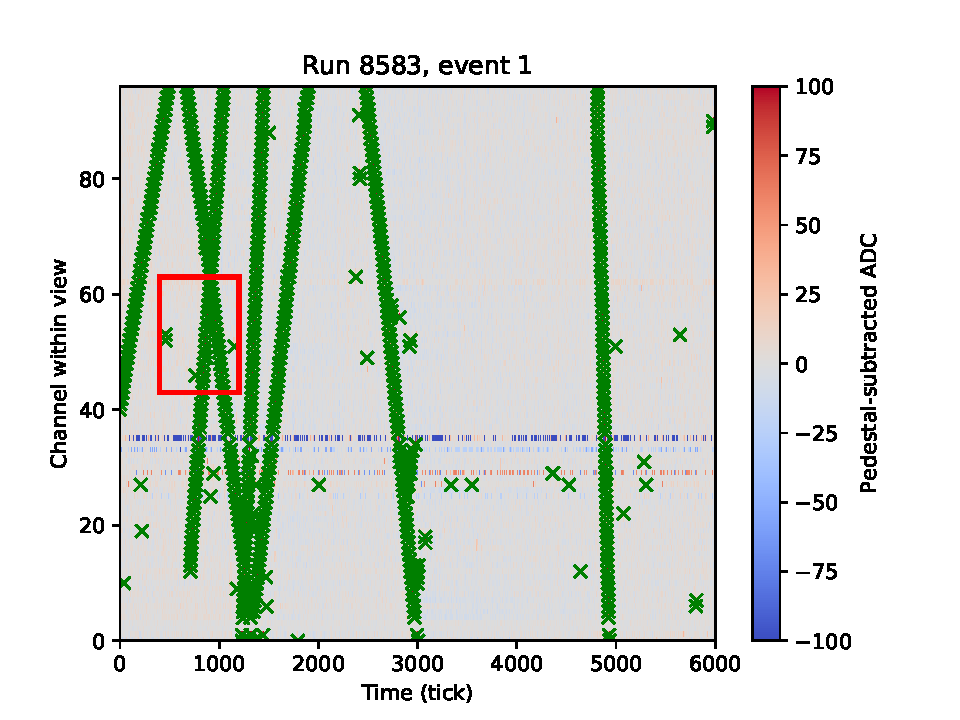
\includegraphics[height=7cm]{raw-event-and-hits-96chans-with-zoom-rect-run8583-evt1.pdf}
    };
    \node[inner sep=0] (zoom) at (4,4) {
      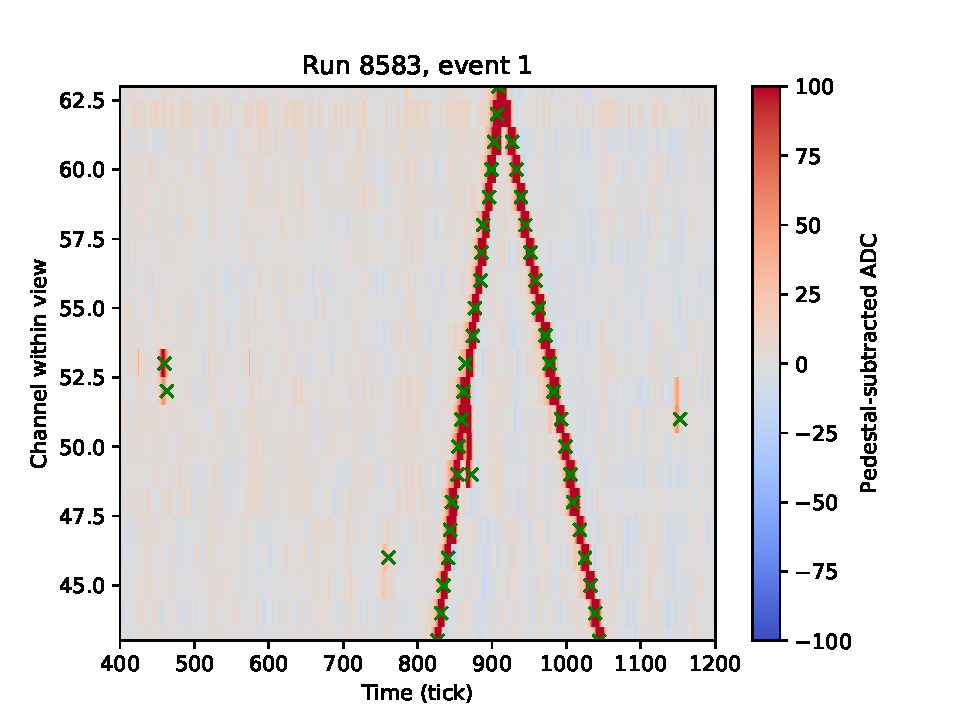
\includegraphics[height=5cm]{raw-event-and-hits-zoom-run8583-evt1.pdf}
    };
    \draw[->, line width=0.3mm, red] (6.25, -.32) -- (1.5, 2.05);
    \draw[->, line width=0.3mm, red] (7.01,  0.8) -- (5.65, 5.9);    
    %\draw[step=1,black,thin,xshift=1,yshift=1] (0,0) grid (10,10);
  \end{tikzpicture}
\end{dunefigure}

\begin{dunefigure}[Trigger primitive rates in ProtoDUNE-SP, four categories]{fig:daq-tp-rates}{Trigger primitive rates in \dword{pdsp} as a function of threshold in four categories: all data (top left),  after removal of particularly noisy channels (top right), with HV off so no contribution to signal (bottom left) and HV off and noisy channels excluded (bottom right).}
  \begin{minipage}[b]{0.5\linewidth}
    \begin{center}
      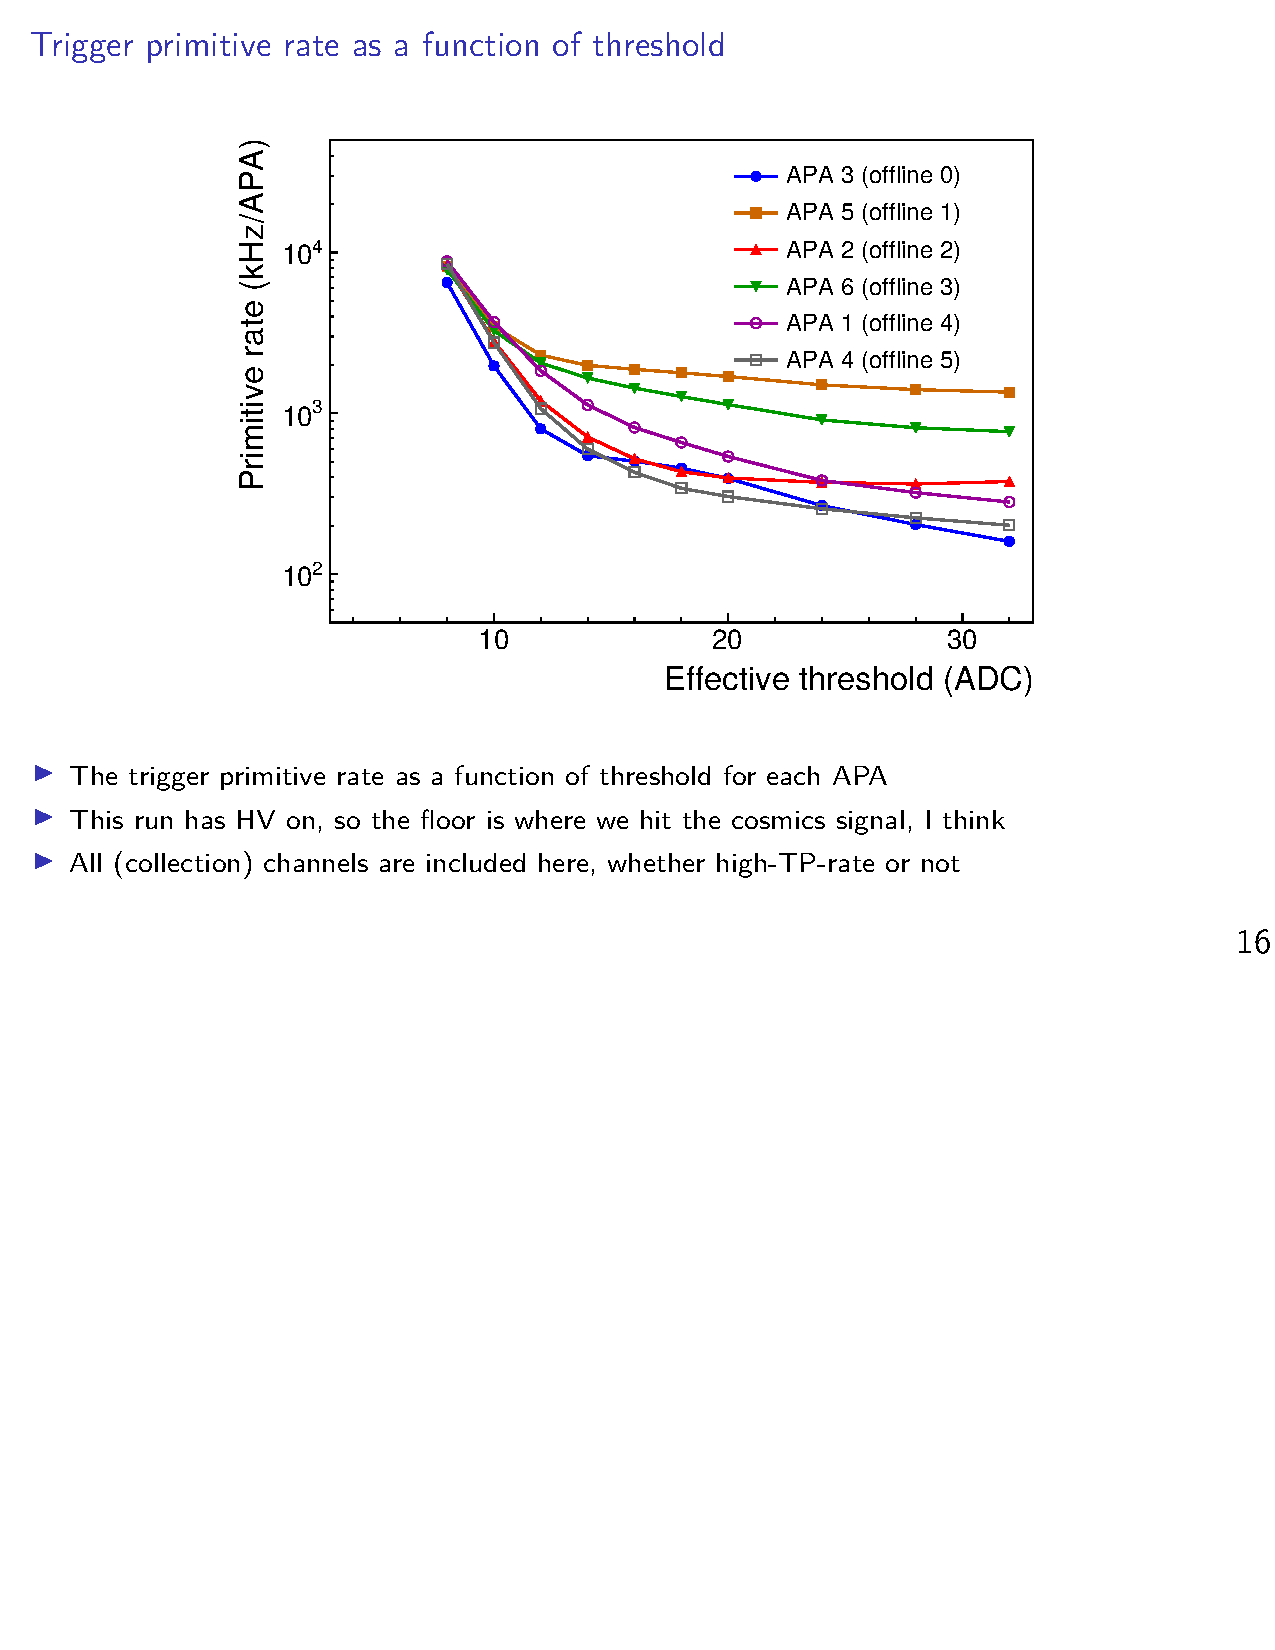
\includegraphics[page=1,width=0.8\textwidth,clip,trim=4cm 16cm 4cm 2cm]{daq-primitive-rates-thresholds.pdf}

      \includegraphics[page=2,width=0.8\textwidth,clip,trim=4cm 16cm 4cm 2cm]{daq-primitive-rates-thresholds.pdf}
    \end{center}
  \end{minipage}%
  \begin{minipage}[b]{0.5\linewidth}
    \begin{center}
      \includegraphics[page=3,width=0.8\textwidth,clip,trim=4cm 16cm 4cm 2cm]{daq-primitive-rates-thresholds.pdf}

      \includegraphics[page=4,width=0.8\textwidth,clip,trim=4cm 16cm 4cm 2cm]{daq-primitive-rates-thresholds.pdf}
    \end{center}
  \end{minipage}

\end{dunefigure}


During early stages of design, significant effort has been dedicated to
trigger primitive generation studies through simulations.
Specifically, charge collection efficiency and fake rates due to noise
and radiologicals have been studied as a function of hit threshold,
demonstrating that requirements can be met, given sufficiently low
electronics noise levels and radiological rates~\cite{bib:docdb11236}. 
Ongoing efforts within DUNE's radiologicals task force aim to validate
or provide more accurate background predictions, against which this
performance will be validated.
In addition, offline studies demonstrate the performance of trigger
primitive generation algorithms as a function of the number of CPU cores
used.  
The results are summarized in Figure~\ref{fig:daq-cpu-hf-speed} and show
that four cores are sufficient to keep up with 960 channels.
The test does not include reformatting of the data required to put it in
a form that allows AVX2 hardware SIMD acceleration.
In tests with live \dword{protodune} data, it is found that ten cores at
and average 65\% usage were enough to handle both reformatting and
trigger primitive selection. 
Effort on understanding and removing contribution
from cosmics/cosmogenics and (known) noisy channels is ongoing.
These results are summarized in Figure~\ref{fig:daq-tp-rates}
Additional details may be found in~\citedocdb{14062}.

\begin{dunefigure}[Efficiency for forming trigger candidates as input trigger primitives]{fig:daq-tc-eff-vis}{Efficiency for forming trigger candidates as input trigger primitives from two algorithms, online (blue) and offline (red).}
  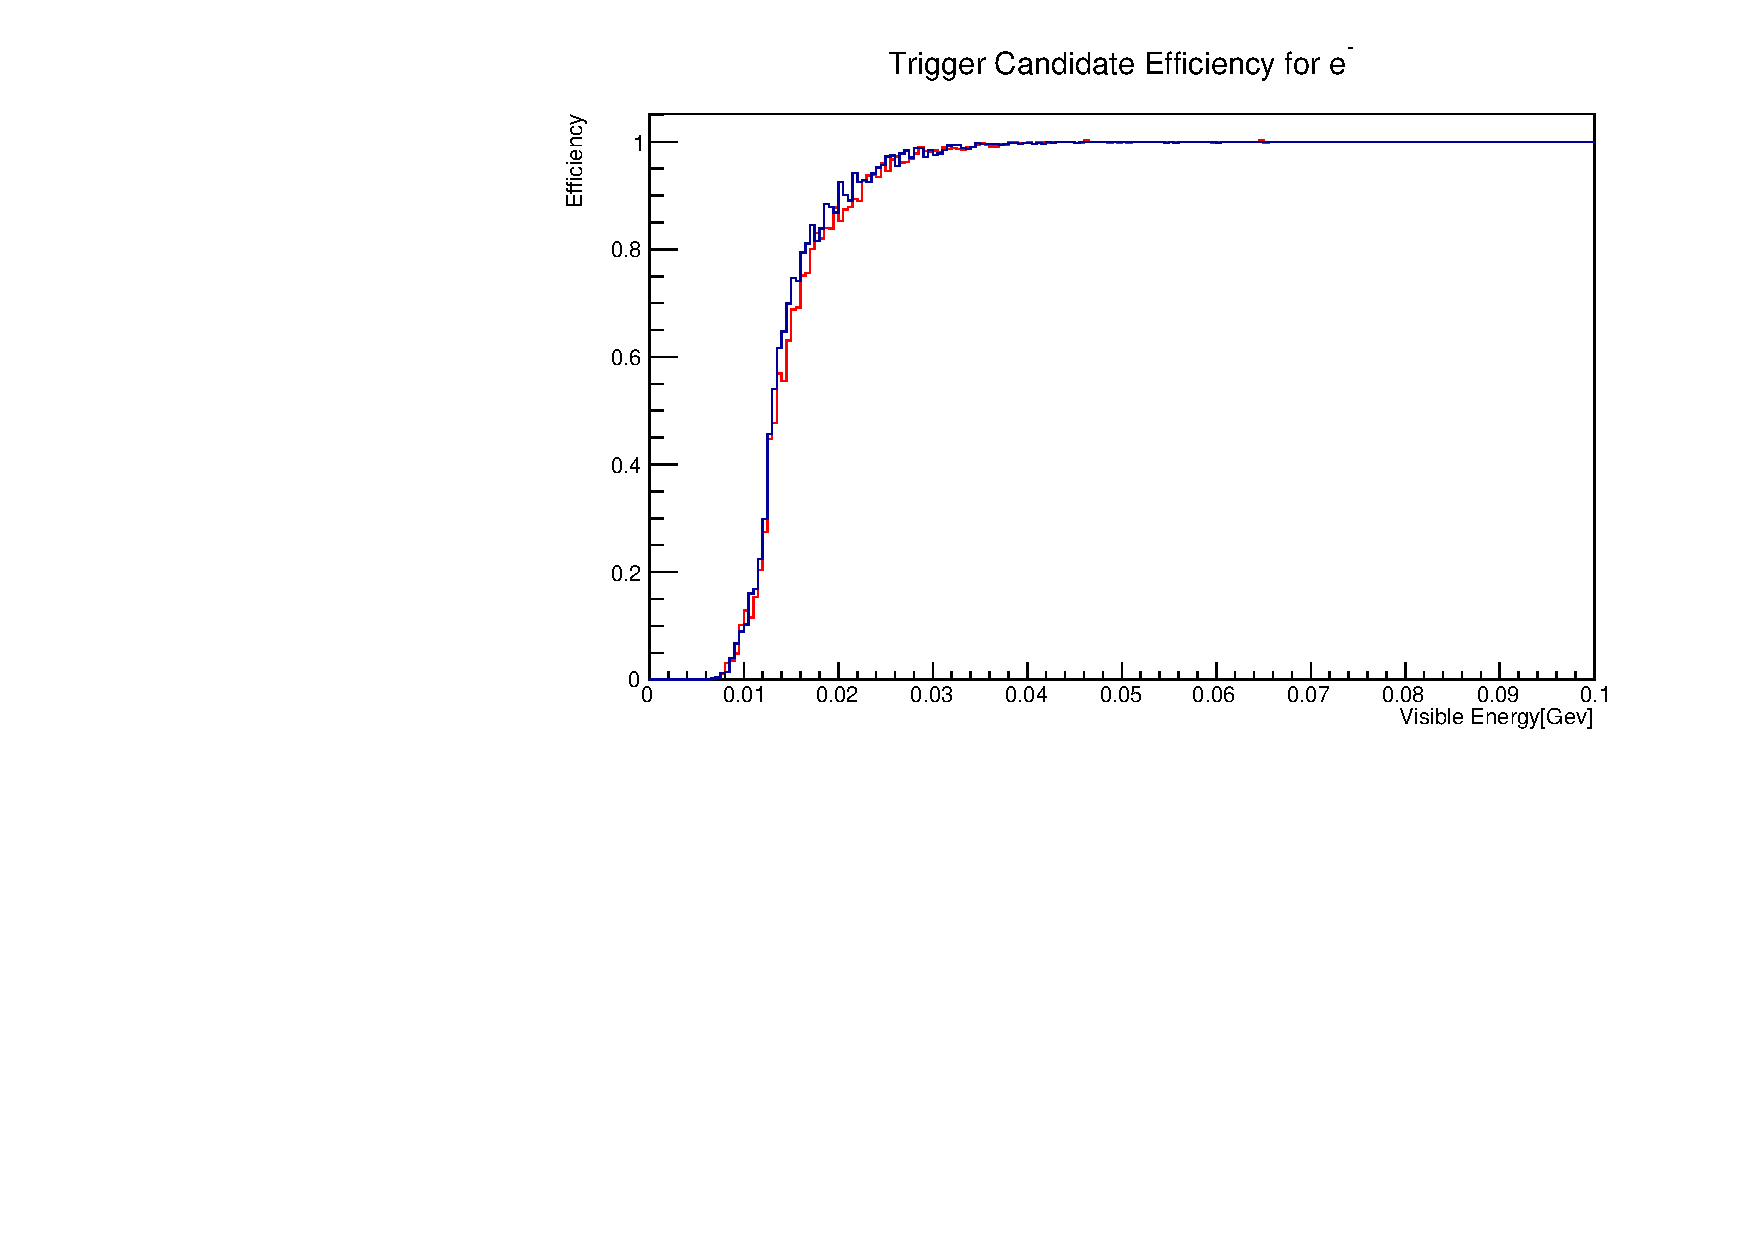
\includegraphics[width=0.7\textwidth]{Electron_Efficiency_Comparison.pdf}
\end{dunefigure}

\begin{dunefigure}[Efficiency for forming trigger candidates from ionization activity]{fig:daq-tc-eff-allinc}{All-inclusive efficiency for
    forming trigger candidates from ionization activity from beam $\nu_e$
    (left) and beam $\nu_\mu$ (right) interactions at or above a given
    visible energy. 
    At smaller energies, somewhat more events with their visible energy
    dispersed in space and time fail the trigger candidate selection
    criteria. 
    High efficiency is obtained at \SI{100}{\MeV} visible. 
    The trigger candidate algorithm used is the offline version, see
    Figure~\ref{fig:daq-tc-eff-vis} for comparison with online version.}
  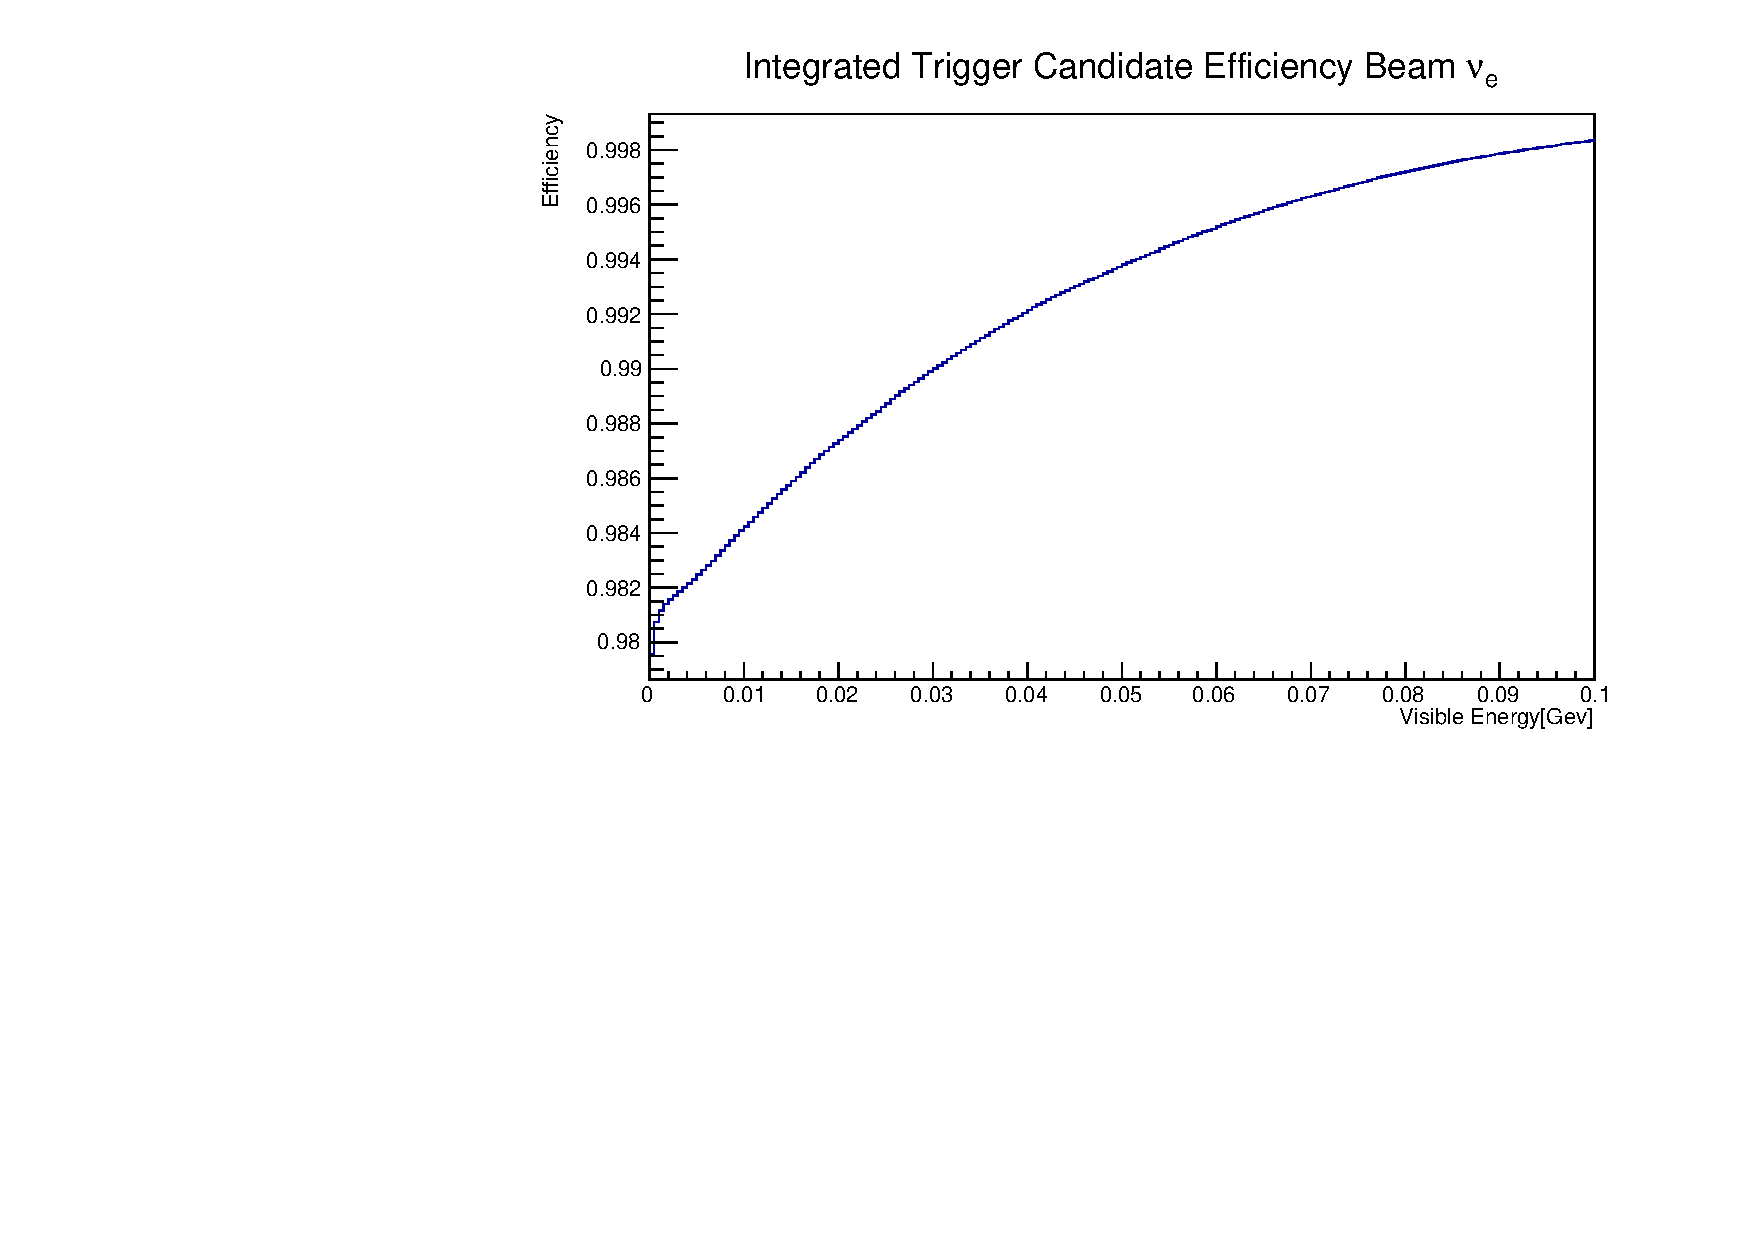
\includegraphics[width=0.45\textwidth]{Integrated_Nu_e_Efficiency_MCC10.pdf}%
  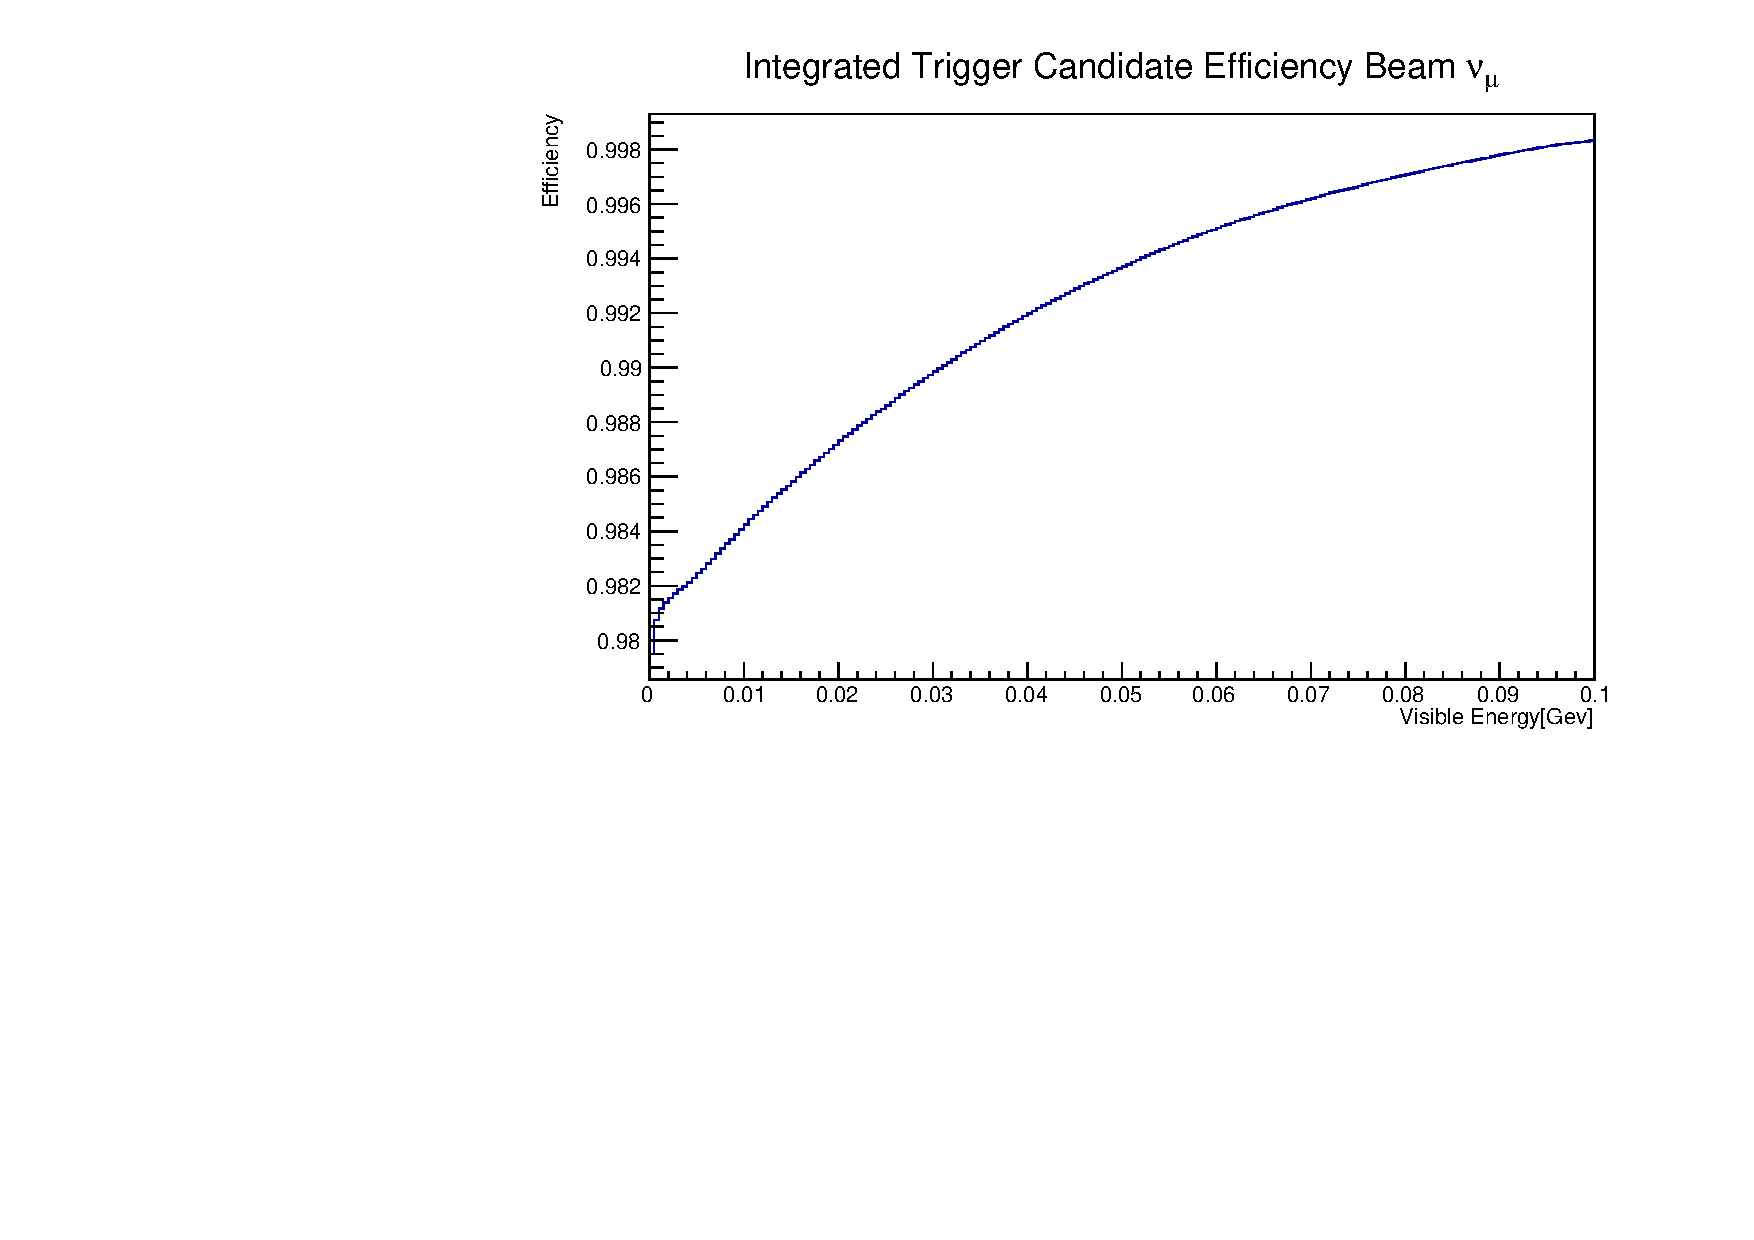
\includegraphics[width=0.45\textwidth]{Integrated_Nu_mu_Efficiency_MCC10.pdf}
\end{dunefigure}


\Dword{trigcandidate} generation, building on trigger primitives information
and considering integral \dword{adc} and trigger primitive proximity by channel
and time (in 50 microseconds) space, has also been studied with Monte
Carlo simulations~\cite{bib:docdb11215}.
Trigger candidates with sufficient total integral \dword{adc}  can be accepted to
generate corresponding \dwords{trigcommand} for localized high energy
activity, such as for beam, atmospheric neutrinos, baryon number
violating signatures, and cosmics.
Simulation studies demonstrate that this scheme meets efficiency
requirements for localized high energy triggers.
Specifically, simulations demonstrate that $>99$\% efficiency is
achievable for $>100$ MeV visible energy deposited by single particles
(shown in Figure~\ref{fig:daq-tc-eff-vis} for $e^-$), and that the
corresponding effective threshold for localized triggers for the system
is at $\sim$10 MeV. This translates to all-inclusive efficiencies for
beam $\nu_e$ and $\nu_\mu$ events in excess of 99\% for visible energies
above 100 MeV, as shown in Figure~\ref{fig:daq-tc-eff-allinc}.

Low-energy \dwords{trigcandidate} furthermore can serve as input to the
SNB trigger. Simulation demonstrates that the trigger candidate
efficiency for any individual \dword{snb} neutrino interaction is on the order
of 20-30\%. Simulations have further demonstrated that a
multiplicity-based \dword{snb} \dword{trigdecision} that integrates low-energy
trigger candidates over an up to 10 seconds
integration window yields high ($>90$\%) galactic coverage while
keeping fake \dword{snb} trigger rates to one per month, in accordance with system
requirements. An energy-weighted multiplicity count scheme could be
applied to further increase efficiency and minimize background.
The dominant contributor to fake \dword{snb} triggers is
radiological backgrounds from neutrons, followed by radon. It is
crucial to continue working closely with the radiological task force
to validate radiological the background assumptions.

In the case of the high level filter, the consortium is exploring the
use of machine learning techniques, specifically image classification
with the use of \dwords{cnn} on GPUs, as a way to
classify and down-select individual sections of \dword{tpc} channel vs. time
(``frames''), with extent of one \dword{apa}'s worth of collection plane
channels by one drift length (2.25 ms, or, 4500 samples). \dwords{cnn} have
been trained on \dword{mc} simulations of frames with each of
the following off-beam event topologies: 
atmospheric neutrino interactions, baryon number violating
interactions (proton decay or neutron-antineutron oscillation), cosmic
ray interactions, supernova neutrino interactions, or no interactions at all -- all
with radiological and noise background included in the
simulations. Preliminary studies show that a \dword{cnn} can be sucessfully trained classify any
given input frame as one of three categories: empty, containing a \dword{snb} neutrino
interaction, or containing a high-energy (atmospheric neutrino, baryon
number violating, or cosmic ray) interaction. Specifically, empty frames can be
rejected with an efficiency of $>$99\%, while frames containing or
partially containing 
a supernova neutrino, an atmospheric/cosmic interaction, or a baryon
number-violating interaction can be preferentially selected with efficiency
$>$88\%, $>$92\%, or $>$99\%, respectively  \cite{bib:docdb11311}. Such a 
filter could potentially be applied to reduce the event record size by
more than two orders of magnitude. Details may be found in~\citedocdb{11311}.
The speed at which machine learning inference may be applied is under study.


\subsubsection{Prototype Trigger Message Passing}

A prototype trigger message passing (PTMP) system using elements of the \dword{ipc} mechanism described in Section~\ref{sec:daq:design-ipc} is currently under development and testing at \dword{protodune}.
The primary goals of this prototype is to add a self-triggering mechanism to the \dword{protodune} detector that includes many of the features needed for the far detector \dword{daq}.
Throughput and latency of the mechanism is being evaluated and optimized.
Message schema and application level protocols have been designed and are being improved.
Future work will include prototyping \dword{daqccm} functionality including \dword{daqdispre}.

PTMP has been successfully exercised to transfer trigger primitives from the software based hit finder. The short-term goal will be to successfully aggregate information from across an APA and feed the result to a trigger candidate finder which identifies horizontal muons. From this output a \dword{trigdecision} can be made.

% \subsection{Additional Teststands}
% \label{sec:sp-daq:validation-demonstrators}

% Concurrently with \dword{pdsp} operation and development, a number of
% ``vertical slice'' teststands will be built to allow 
% development and testing of individual parts of the \dword{daq} system
% as well as testing of key aspects of the design and overall
% scalability. A data selection subsystem vertical slice teststand will be
% constructed and operated on fake-generated data, to assist in the
% development of data selection, exercise the system for a variety of
% configurations, perform small-scale tests that stress the critical
% parts of the corresponding infrastructure, 
% and identify likely failure points and/or bottlenecks. The subsystem
% will also be deployed and exercised on existing HPC clusters of
% comparable resources and specifications as planned for the final
% production system for ``horizontal slice'' tests of similar nature. The
% \dword{daqbes} will be developed and tested in a similar way.

% In addition to dedicated vertical and horizontal slice teststands, a number of
% \dword{daq} development kits will be available for the consortium for
% specific component testing, as well as to other detector and
% calibration consortia to support their own development, production, and quality assurance programs. The \dword{daq} 
% kit will also form the basis for testing at \dword{apa} Construction sites beginning in 2020. 

\subsection{Plan for Future Development}
\label{sec:sp-daq:design-plans}

As mentioned in the introduction of this section, at present, the development model chosen for the \dword{daq} system is the one of iterative prototyping.
This model is widely used in projects in which requirements are still
being refined and particularly for systems relying on rapidly evolving technologies, such as today's information and computing sector. 
This model will be used throughout 2019, making use of the \dword{protodune} setup to explore architectural options, software solutions, etc.
At a later stage, the \dword{daq} development will move to a more streamlined incremental model, ensuring that careful design precedes the final implementation of individual components.
Most of the development will be carried out emulating the data inputs.
On the other hand, the \dword{daq} will be validated regularly via test stand integration with detectors, such as \dword{protodune} or pre-installation sites.
The overall development schedule with the main \dword{daq} milestones is shown in Section~\ref{sec:fd-daq:schedule}.

\section{Production, Assembly, Installation and Integration}
\label{sec:sp-daq:production}

The \dword{daq} system relies largely on commercial off the shelf components, with the exception of the timing system and the first stage of the upstream \dword{daq}.
Therefore, the production and assembly aspects are simpler than for other systems, while of course the installation and integration stages are very important and have to be planned carefully, due to the large number of interfaces of the \dword{daq} system with other parts of the experiment.

\subsection{Production and Assembly}
\subsubsection{Timing System}
A prototype of the timing system already exists and has been used at \dword{pdsp}. The final hardware prototype will be used in the second run of \dword{pdsp} in 2021 and production is planned right afterwards, allowing detector communities to have an early integration with the timing hardware and firmware.

\subsubsection{Upstream DAQ}
The upstream \dword{daq} will have FPGA mezzanine cards connecting to the detector electronics readout fibres, and processing and storing data temporarily. Prototype cards implementing parts of the required functionality exist already, but more prototypes are planned before the production readiness review planned in December 2022. While the hardware design will be done at the institutions working in this area, the production of prototypes and final cards will be outsourced to companies, allowing for early identification of those companies that can guarantee a high quality cards production.

\subsubsection{Racks, Servers, Storage and Network}
While commercial devices do not need to be produced or assembled, enough time has to be planned, once the proper devices are identified, for the tendering and procurement procedures. Racks and fibers will be procured in order to be available early in 2023; servers and switches will be purchased in two batches, one to be ready for supporting the installation and commissioning of the detector components and \dword{daq} infrastructure and one to reach nominal performance, in time for the start of data taking.

\subsection{Installation and Integration}

%\metainfo{Describe how we get stuff in place underground, how we will put it all together and make sure it works. 
%  What can we do to minimize the effort needed underground both in
 % terms of physical work but also in working out the bugs both in
 % individual processes and in emergent behavior of the system as a
 % whole?}

The \dword{daq} will be installed in an enclosure in the west end of the Central
Utilities Cavern (\dword{cuc}) (Figure~\ref{fig:cavern-layout}).  Roughly
half of this space will be office space (including control
workstations) and the other will be a computer room to hold the \dword{daq}
front-end computing and network equipment (Figure~\ref{fig:install-cuc}). Further details of the interface of \dword{daq} with underground facilities
may be found in \citedocdb{6988}, and the installation interface document for \dword{daq} in \citedocdb{7015}.

% TDR refs DocDB, not EDMS.  EDMS is only a "working area".
% \fixme{Docdb 7105 is obsolete, refers to https://edms.cern.ch/document/2145183}

Infrastructure in the \dword{cuc} will be installed starting in Q4~2022
(Figure~\ref{fig:high-level-schedule}).  At that point, CF will have
handed the \dword{daq} group an empty room with cooling water and power
connections.  Over the next nine months, racks for the \dword{daq} computing
will be installed, plumbed into cooling water, and connected to power
and networking.  The network connection from this data room to the fiber
trunks going up the shaft will also be made, as will preparations to
receive the multi-mode fiber connections from the \dword{wib} to the
\dword{felix} cards housed in servers in these racks. There is space
for \cucracks racks, with 4 set aside for other consortia, 12 per
module for upstream \dword{daq} electronics, and the remaining space for
networking and other \dword{daq} computing needs. An initial engineering design of the computer room is shown in Figure~\ref{fig:daq-room}, which meets all requirements for capacity, cooling, safety and installation schedule.

\begin{dunefigure}[DAQ counting room in the CUC]{fig:daq-room}{Initial engineering design for the \dword{daq} counting room in the CUC}
  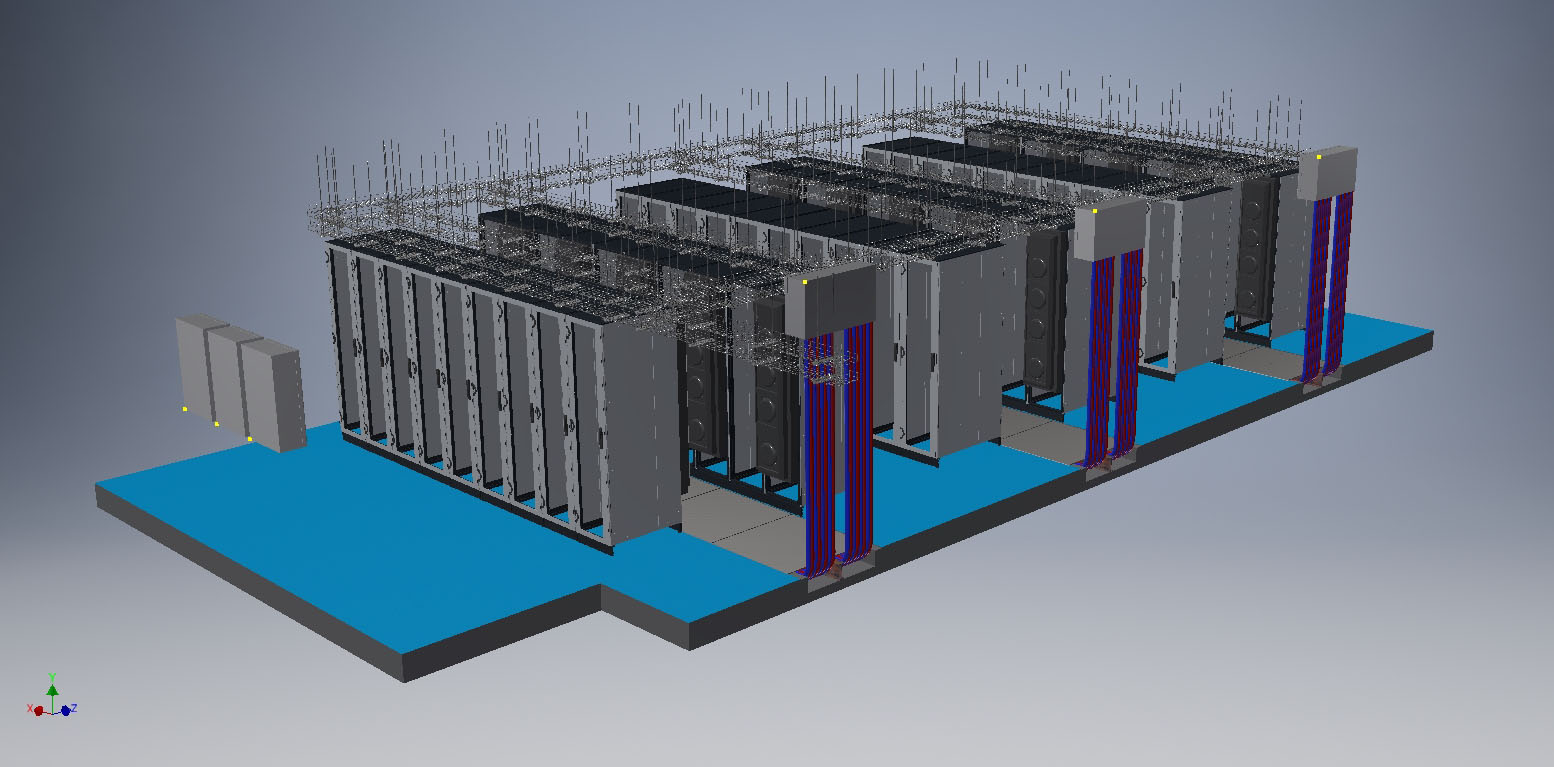
\includegraphics[width=0.9\textwidth]{daq-room.jpg}
\end{dunefigure}

Starting in Q3~2023, the data room will be ready for the installation of
the \dword{daq} servers servicing the first module described in
Section~\ref{sec:fd-daq:considerations}.  This will proceed over the
next year, with servers being installed, cabled up, and tested.
As much configuring and commissioning work as possible will be done over
the network from the surface (or home institutions), to limit the number
of people underground.  Note that this data room is sized for all four
modules of \dword{daq} computing, so one quarter will be installed at this
point.  If more computing power is needed for the commissioning of the
first module (for example, to deal with unexpected noise levels), space
and power will be borrowed from the provision for future modules until the problems are
alleviated. 
Additional space for eight racks will be on the surface in the Ross Dry
Room. This will house the back-end computers, high level filter servers, and associated network equipment.

Starting in Q3~2024, the \dword{daq} will thus be ready to connect fibers to the
\dwords{wib} on the detector top as planes are installed, to allow their commissioning.

The underground installation phase of the \dword{daq} system has the largest safety
implications, which are discussed in Section~\ref{sec:fd-daq:safety}.

\section{Organization and Project Management}
\label{sec:sp-daq:organization}


\subsection{Consortium Organization}

The \dword{daq} consortium was formed in 2017 as a joint single and
dual phase consortium, with a consortium leader and a technical
leader. The current organization of the consortium is shown in
Figure~\ref{fig:daq-org}. The \dword{daq} institution board currently comprises
representatives from 34 institutions as shown in Table~\ref{tab:daq-ib}. The consortium leader is the spokesperson for the consortium and responsible for the overall scientific program and management of the group. The technical leader of the consortium is responsible for
managing the project for the group. The leadership is assisted in its duties by the Project Office, populated by the Resource Manager, the Software and Firmware coordinator and the Integration and Support Coordinator, providing support in the corresponding areas. 
The consortium is organized into working groups addressing the design,
R\&D, integration, and, in the future, construction, commissioning and installation of the key \dword{daq} systems. The Physics Performance and Facility working groups are not associated to a specific system but provide oversight of the general \dword{daq} performance in the physics context and the on the interface with the facility infrastructure. The \dword{daq} working group mandates are detailed in~\citedocdb{14938}.

\begin{dunefigure}[DAQ consortium org chart]{fig:daq-org}{Organizational chart for the \dword{daq} Consortium
}
  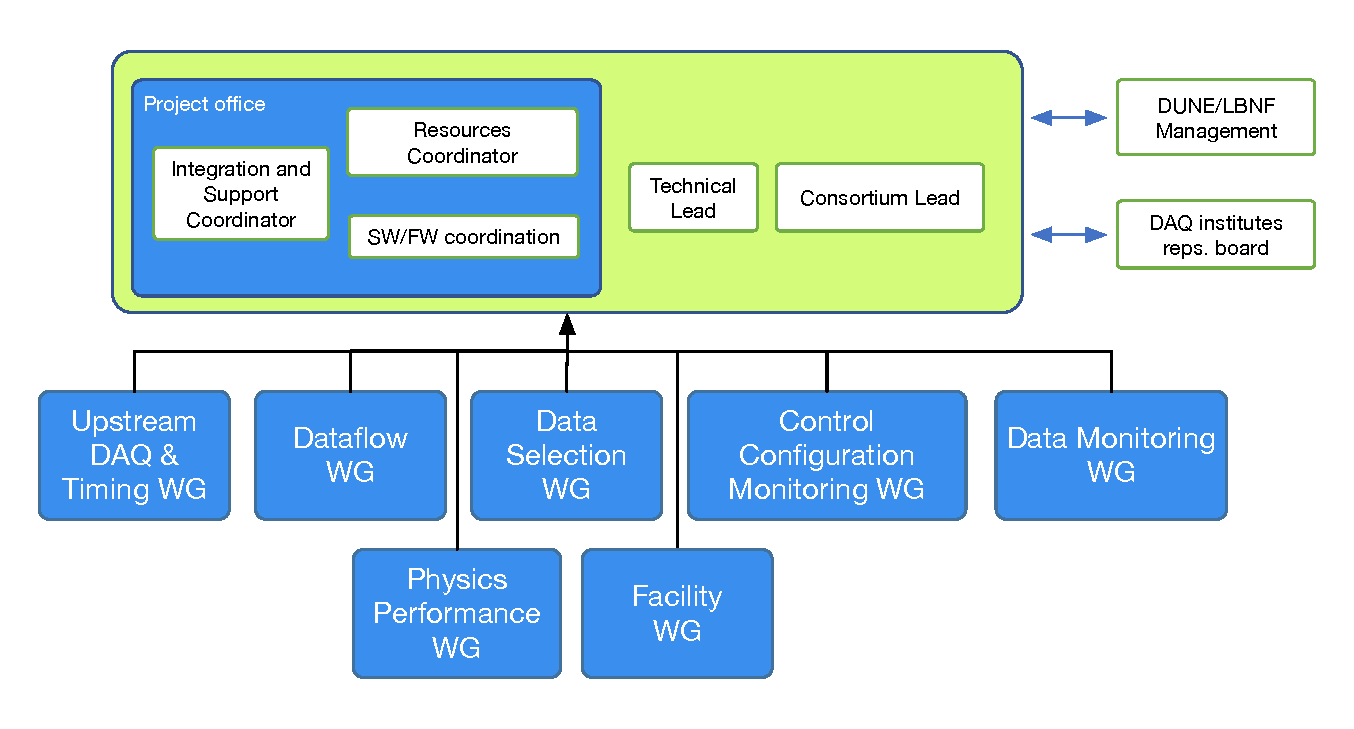
\includegraphics[width=0.9\textwidth]{daq-organogram.pdf}
\end{dunefigure}

\begin{dunetable}
[DAQ Consortium Board institutional members and countries]
{p{0.65\textwidth}p{0.25\textwidth}}
{tab:daq-ib}
{DAQ Consortium Board institutional members and countries.}   
Member Institute & Country  \\ \toprowrule
CERN & CERN     \\ \colhline
Universidad Sergio Arboleda (USA) & Colombia     \\ \colhline
Czech Technical University & Czech Republic \\ \colhline
Lyon & France \\ \colhline
INFN Bologna & Italy \\ \colhline
Iwate & Japan     \\ \colhline
KEK & Japan     \\ \colhline
NIT Kure & Japan     \\ \colhline
NIKHEF & Netherlands    \\ \colhline
University of Birmingham & UK     \\ \colhline
Bristol University & UK     \\ \colhline
University of Edinburgh & UK     \\ \colhline
Imperial College London & UK     \\ \colhline
University College London (UCL) & UK     \\ \colhline
University of Liverpool & UK     \\ \colhline
Oxford University & UK     \\ \colhline
Rutherford Appleton Lab (RAL) & UK     \\ \colhline
University of Sussex & UK     \\ \colhline
University of Warwick & UK     \\ \colhline
Brookhaven National Lab (BNL) & USA     \\ \colhline
Colorado State University (CSU) & USA     \\ \colhline
Columbia University  & USA     \\ \colhline
University of California, Davis (UCD) & USA     \\ \colhline
Duke University & USA     \\ \colhline
University of California, Irvine (UCI) & USA     \\ \colhline
Fermi National Accelerator Laboratory (Fermilab) & USA     \\ \colhline
Iowa State University & USA     \\ \colhline
University of Minnesota, Duluth (UMD) & USA     \\ \colhline
University of Notre Dame & USA     \\ \colhline
University of Pennsylvania (Penn) & USA     \\ \colhline
South Dakota School of Mines and Technology (SDSMT) & USA     \\ \colhline
Stanford Linear Accelerator Lab (SLAC) & USA     \\ \colhline
\end{dunetable}


\subsection{Schedule and Milestones}
\label{sec:fd-daq:schedule}

The high-level \dword{daq} milestones are listed in Table~\ref{tab:daq-sched}, interleaved with the top-level DUNE project milestones, and illustrated in Figure~\ref{fig:fd-daq:schedule}. Since the \dword{daq} project is largely based on commercial off-the-shelf components, it can be seen in the overall timeline that many of the components are procured relatively late in the project schedule.

\begin{dunetable}
[DAQ Consortium Schedule]
{p{0.65\textwidth}p{0.25\textwidth}}
{tab:daq-sched}ane 
{\dword{daq} Consortium Schedule}   
Milestone & Date (Month YYYY)   \\ \toprowrule

Upstream \dword{daq} Architecture Technology Decision & June 2020 \\ \colhline
Engineering Design Review for Timing System &  June 2020   \\ \colhline
\rowcolor{dunepeach} Start of \dword{pdsp}-II installation& \startpduneiispinstall      \\ \colhline
Production Readiness Review for Timing System & June 2021 \\ \colhline
Preliminary Software Design Review & January 2022 \\ \colhline
Engineering Design Review for Hardware/Firmware & March 2022 \\  \colhline
\rowcolor{dunepeach} Start of \dword{pddp}-II installation& \startpduneiidpinstall      \\ \colhline
\rowcolor{dunepeach}South Dakota Logistics Warehouse available& \sdlwavailable      \\ \colhline
%\dword{prr} dates & December 2021 \\ \colhline
%Production Readiness Review Dates &  January 2022   \\ \colhline
Start of Racks Procurement & July 2022  \\ \colhline
Start of \dword{daq} Server Procurement (I) & September 2022  \\ \colhline
\rowcolor{dunepeach}Beneficial occupancy of cavern 1 and \dword{cuc}& \cucbenocc      \\ \colhline 
Production Readiness Review for Readout Hardware/Firmware & December 2022  \\ \colhline
End of Racks Procurement & March 2023  \\ \colhline
Start of  \dword{daq} Custom Hardware Production &  March 2023    \\ \colhline
\rowcolor{dunepeach} \dword{cuc} counting room accessible& \accesscuccountrm      \\ \colhline
End of \dword{daq} Server Procurement (I) & May 2023  \\ \colhline
Start of \dword{daq} Installation & May 2023 \\ \colhline
\dword{daq} Software Final Design Review & June 2023  \\ \colhline

End of  \dword{daq} Custom Hardware Production &  December 2023    \\ \colhline
\rowcolor{dunepeach}Top of \dword{detmodule} \#1 cryostat accessible& \accesstopfirstcryo      \\ \colhline
\rowcolor{dunepeach}Start of \dword{detmodule} \#1 TPC installation& \startfirsttpcinstall      \\ \colhline
Start of \dword{daq} Server Procurement  (II) & September 2024  \\ \colhline
\rowcolor{dunepeach}Top of \dword{detmodule} \#2 accessible& \accesstopsecondcryo      \\ \colhline

End of \dword{daq} Server Procurement  (II) & May 2025  \\ \colhline
End of \dword{daq} installation & May 2025 \\ \colhline
\rowcolor{dunepeach}End of \dword{detmodule} \#1 TPC installation& \firsttpcinstallend      \\ \colhline
 \rowcolor{dunepeach}Start of \dword{detmodule} \#2 TPC installation& \startsecondtpcinstall      \\ \colhline
End of \dword{daq} Standalone Commissioning & December 2025 \\ \colhline
\rowcolor{dunepeach}End of \dword{detmodule} \#2 TPC installation& \secondtpcinstallend      \\ \colhline
\dword{daq} Server Procurement  (III) & July 2026  \\ \colhline
End of \dword{daq} Commissioning & December 2026  \\ 
\end{dunetable}

\begin{dunefigure}[DAQ schedule for first \SI{10}{\kilo\tonne} module]{fig:daq-schedule}{\dword{daq} schedule for first \SI{10}{\kilo\tonne} module. \label{fig:fd-daq:schedule}}
  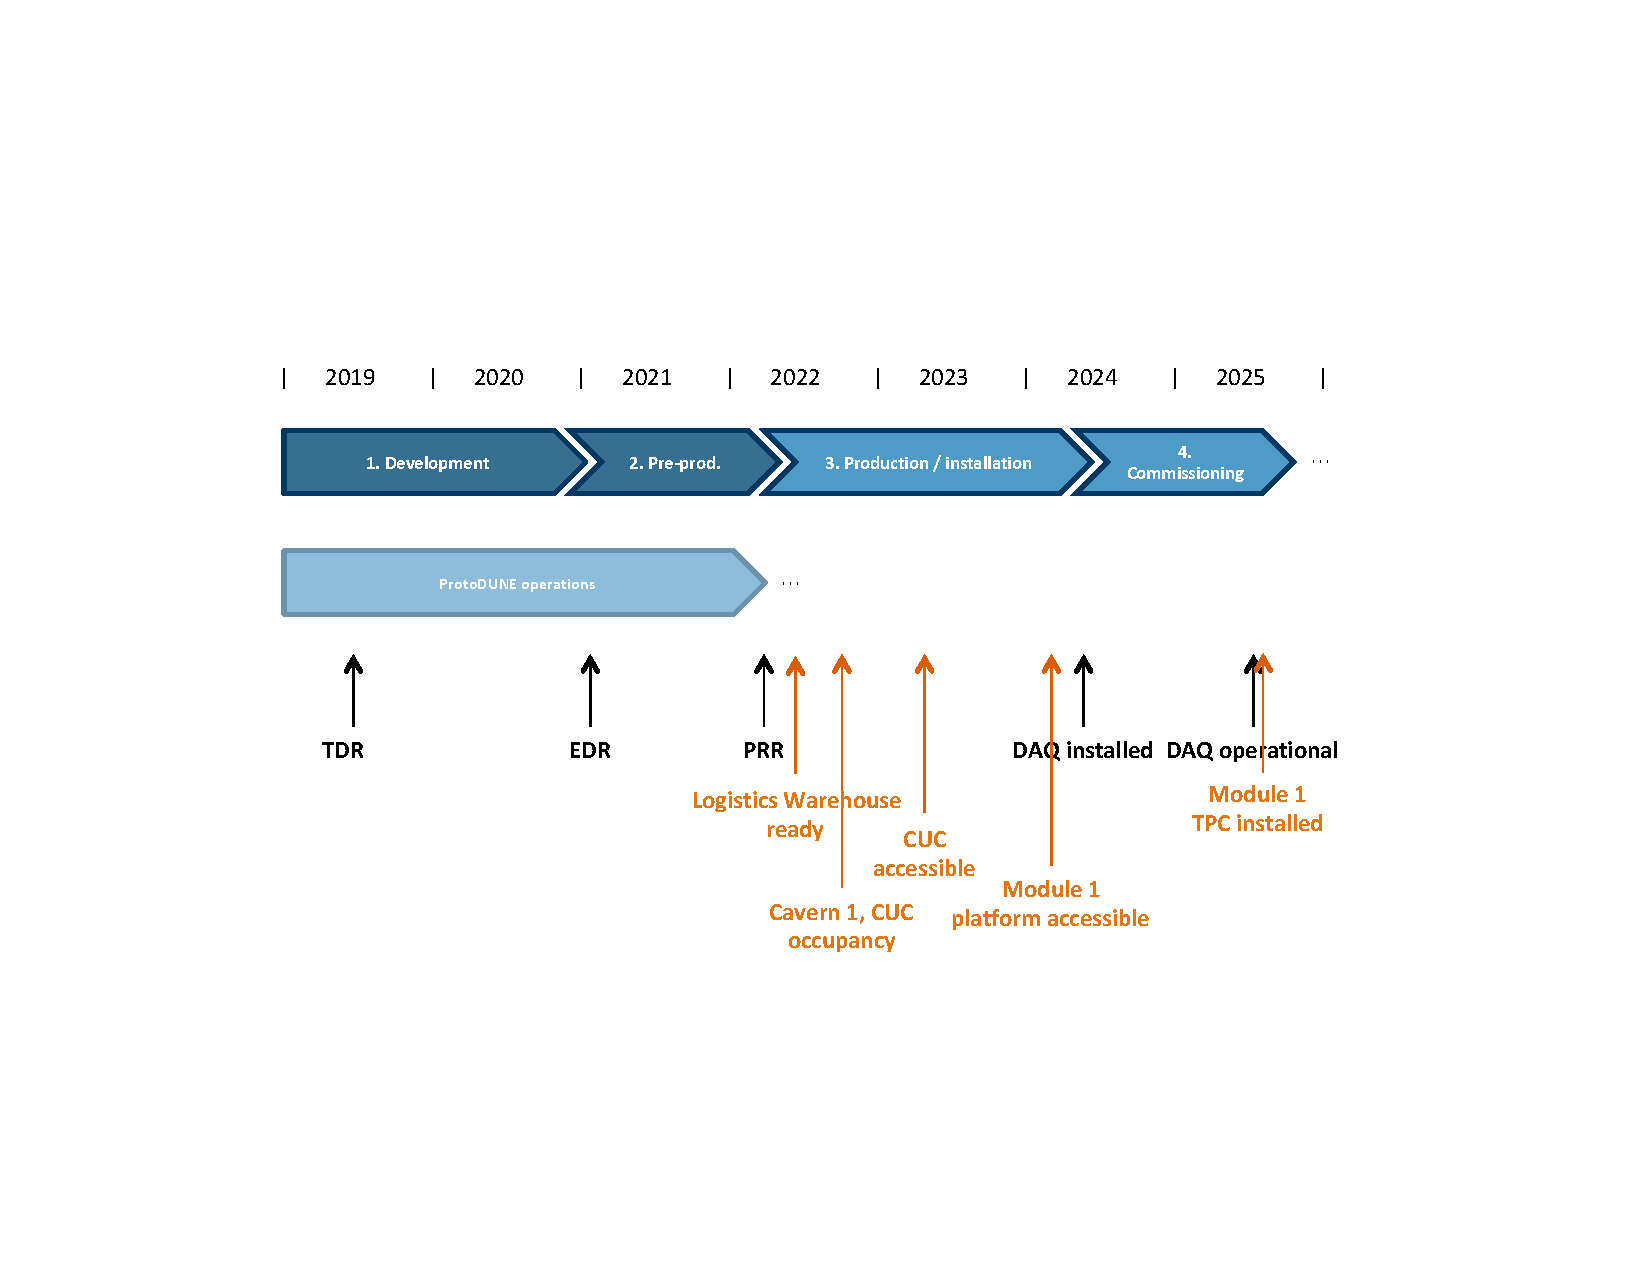
\includegraphics[width=0.95\textwidth,clip,trim=1cm 2cm 1cm 2cm]{daq-schedule.pdf}
\end{dunefigure}


\subsection{Safety and Risks}
\label{sec:fd-daq:safety}

Personnel safety during design, construction, testing, installation, and
commissioning of the system is crucial for the success of the
project. Detector safety during installation,
commissioning and operations is also key to project success.
The consortium will strictly follow ES\&H guidelines for the
project as well as follow the safety rules of the institutions where
the work is performed, including national laboratories, SURF, and
participating universities.  

Two overall safety plans will be followed by the FD \dword{daq}. General work underground will comply
with all safety procedures in place for working in the detector
caverns and in the \dword{cuc} underground at
SURF. \dword{daq}-specific procedures for working with racks full of
electronics or computers, as defined 
at Fermilab, will be followed, especially with respect to electrical safety and the fire suppression
system chosen for the counting room. For example, a glass wall between the server room space and
the other areas in the CUC will be necessary to prevent workers in the server room from being
unseen if they are in distress, and an adequate hearing protection
regime must be put in place.

There are no other special safety items for the \dword{daq} system not already covered by the more general safety plans. The long-term emphasis is on remote operations capability from around the world, limiting the need for physical presence at SURF, and with underground access required only for urgent interventions or hardware replacement. 

A set of risks to the successful construction and operation of the \dword{daq} system has been
identified by the consortium, and is provided,
together with mitigation strategies and pre-mitigation risk level, 
in Table~\ref{tab:risks:SP-FD-DAQ}. Post-mitigation risk levels are
currently being re-evaluated. Risk is quantified with respect to
probability, cost impact, and schedule impact. High (H), medium (M), and low (L)
probability is identified as
$>25$\%, $10-25$\%, and $<10$\%, respectively; high (H), medium (M), and low (L)
cost impact is identified as
$>20$\%, $5-20$\%, and $<5$\% cost increase, respectively; and high
(H), medium (M), and low (L) schedule impact is identified as 
$>6$ months, $2-6$ months, and $<2$ months delay, respectively.


% risk table values for subsystem SP-FD-DAQ
\begin{longtable}{p{0.18\textwidth}p{0.20\textwidth}p{0.32\textwidth}p{0.02\textwidth}p{0.02\textwidth}p{0.02\textwidth}} 
\caption{Risks for SP-FD-DAQ \fixmehl{ref \texttt{tab:risks:SP-FD-DAQ}}} \\
\rowcolor{dunesky}
ID & Risk & Mitigation & P & C & S  \\  \colhline
RT-SP-DAQ-01 & Detector noise specs not met & ProtoDUNE experience with noise levels and provisions for data processing redundancy in DAQ system (upstream DAQ FPGA/CPU and high level filter) & H & M & H  \\  \colhline
RT-SP-DAQ-02 & Externally-driven schedule change & Provisions for standalone testing and commissioning of production DAQ components, and schedule adjustment & H &  & M \\  \colhline
RT-SP-DAQ-03 & Lack of expert personnel & Resource-loaded plan for DAQ backed by institutional commitments, and schedule adjustment using float & H &  &  \\  \colhline
RT-SP-DAQ-04 & Power/space requirements exceed CUC capacity & Sufficient bandwidth to surface and move module 3/4 components to an expanded surface facility & H & M & H \\  \colhline
RT-SP-DAQ-05 & Excess fake trigger rate from instrumental effects & ProtoDUNE performance experience, and provisions for increase in event builder, high level filter, and upstream DAQ processing capacity, as needed & M & M & H  \\  \colhline
RT-SP-DAQ-06 & Calibration requirements exceed acceptable data rate & Provisions for increase in event builder and high level filter capacity, as neeed & M & L & M \\  \colhline
RT-SP-DAQ-07 & Cost/performance of hardware/computing excessive & Have prototyping and pre-production phases, reduce performance using margin or identify additional funds & M &  &  \\  \colhline
RT-SP-DAQ-08 & Optical components obsolete before production & Market survey, commercial standards, and design changes & H  &  &  \\  \colhline
RT-SP-DAQ-09 & Insufficient FPGA processing resources & ProtoDUNE and simulation experience, FPGA replacement, or sustain increased data rates & H  & H  & H  \\  \colhline
RT-SP-DAQ-10 & Insufficient throughput in computing system & Design allows for expansion; expand system capacity for throughput before commissioning & H  & M & H  \\  \colhline
RT-SP-DAQ-11 & Event builder throughput insufficient & Design allows for expansion; expand system capacity for throughput before commissioning & H  & M & M \\  \colhline
RT-SP-DAQ-12 & Additional data reduction steps required after event building & Provisions for increase in high level filter capacity, as needed & H  & L & M \\  \colhline
RT-SP-DAQ-13 & PDTS fails to scale for DUNE requirements & Hardware upgrade & M & L & H  \\  \colhline
RT-SP-DAQ-14 & Full remote operation of DAQ proves non-viable & Pre-production operation testing and allocation of surface or underground space for on-site operations & M &  & M \\  \colhline
RT-SP-DAQ-15 & DAQ system does not meet overall DUNE uptime specification & Extensive QA and exercise of failure mode recovery in extended ProtoDUNE runs, and replacement of components & H  &  & M \\  \colhline
RT-SP-DAQ-16 & External services do not allow reliable operation of DAQ system & Performance specifications for external services, prior to construction. & H  & L & H  \\  \colhline

\label{tab:risks:SP-FD-DAQ}
\end{longtable}

The following risks and mitigation strategies have been identified:

\begin{description}
\item[Detector noise specs not met] Excessive noise will make it
  impossible for the \dword{daqdss} to meet physics goals while
  generating reasonable data volumes. Prior (to construction) mitigation includes
  studying noise conditions at \dword{protodune}, and leaving provisions in the
  system for additional front-end filtering (in the form of the
  upstream \dword{daq} upgradable processing resources) and/or post-event builder processing (in
  the form of the high level filter). Mitigation (post-construction) includes augmenting
  filtering resources using a larger computing system for the high
  level filter.

\item[Externally-driven schedule change] The \dword{daq} has schedule links during
  testing, construction, and installation phases with most other
  subsystems. Schedule slip elsewhere will potentially cause
  delay to the \dword{daq}. Prior mitigation includes making provisions for
  stand-alone testing and commissioning of \dword{daq} components, in the form
  of vertical and horizontal slice tests, at \dword{protodune} or
  elsewhere. Mitigation includes adjusting schedule for stand-alone
  testing and commissioning phases. 

\item[Lack of expert personnel] A significant number of experts in
  hardware, software, firmware are needed, and must be sustained
  throughout the project. Lack of personnel will increase technical
  risks and cause delay. Prior mitigation includes developing a full
  resource-loaded plan for \dword{daq}, backed by national and institutional
  commitments, and avoiding single points of failure. Mitigation
  includes adaptation of the \dword{daq} schedule, using schedule float.

\item[Power/space requirements exceed CUC capacity] The CUC has fixed
  space and power allocation for \dword{daq} 
that cannot be exceeded.  Prior mitigation includes allowing
sufficient bandwidth up the shafts to move the upstream \dword{daq} components for
subsequent DUNE far detector modules (modules 3 and 4) to the
surface, or moving some of the \dword{daq} components to the detector caverns,
and carrying out a feasibility study for doing so. 
Mitigation includes expending additional resources on an
expanded surface facility.

\item[Excess fake trigger rate from instrumental effects] Instrumental
  effects (beyond excessive noise) can cause fake triggers. Prior
  mitigation includes studying \dword{protodune} performance in detail, and monitoring detector
  performance during installation. Mitigation includes substantially increasing
  data volume, and increasing processing resources in the high level
  filter.

\item[Calibration requirements exceed acceptable data rate]
  Calibration schemes may require substantial data 
volumes, far in excess of triggered data volume, beyond currently
envisioned; e.g., due to offline analysis inefficiencies. Prior
mitigation includes allowing for back-end (\dword{eb}) system expansion to cope
with the increased data rate, and allowing for a high-level filter data
selections stage to carry out online analysis and data
reduction. Mitigation includes increasing the back-end \dword{daq} and high
level filter system capacity. 

\item[Cost/performance of hardware/computing excessive] Costs of
  system-as-designed may exceed available budget, due to the IT technology (FPGA, servers, storage) market evolving in an unfavorable way. Prior mitigation
  includes the planning of prototyping and pre-construction phases to allow
  realistic appraisal of system costs, and applying sufficient margin
  in performance estimates.  Mitigation includes reducing performance
  or identifying additional funds. 

%\item[Optical components obsolete before production] Chosen data
%  transmission technology may be 
%obsolete (e.g. parallel 1Gb/s receivers). Prior mitigation includes
%conducting a thorough market survey before the final design choices
%for front-end electronics and DAQ interface technology, and sticking
%to commercial standards. Mitigation 
%includes change of design for both DAQ and front-end electronics.

%\item[Insufficient FPGA processing resources] FPGA processing
 % resources may be found to be
%insufficient after construction. Prior mitigation includes a careful
%assessment of resource needs in situ at ProtoDUNE and through
%simulation, as well as allowing for an upgrade of the system via FPGA
%replacement. Mitigation includes replace FPGAs or sustaining higher
%data rates through the system.

%\item[Insufficient throughput in computing system] The computing system
 % as-constructed may not scale to meet throughput requirements of
 % DAQ. Prior mitigation includes designing the system so as to allow
%   for expansion of resources as required (i.e.~by avoiding
%   single-point bottlenecks). Mitigation includes expanding the system capacity before commissioning. 

% \item[Event builder throughput insufficient] The event builder system
%   as-constructed may not scale to 
% meet throughput requirements of DAQ.  Prior mitigation includes
% designing the system so as to allow for expansion of resources
% (i.e.~by avoiding single-point bottlenecks). Mitigation includes
% expanding the system capacity before commissioning.

% \item[Additional data reduction steps required after event buiding] An
%   additional step of data reduction or online filtering
%  or analysis may be required, after the event building step, beyond
%  what can be accommodated in high level filter. Prior mitigation
%  includes the provision for a scalable high level filter on
%  surface. Mitigation includes expanding the high level filter
%  resources.

\item[\dword{protodune} timing system fails to scale for DUNE requirements] The \dword{protodune} timing system concept may
  not scale to DUNE in scale or performance.  Prior mitigation
  includes testing the system at realistic scale before the final
  design. Mitigation includes replacing the system with upgraded
  hardware.

% \item[Full remote operation of DAQ proves non-viable] The DAQ consoritum
%   concept is for remote operations 
%  with on-site maintenance activities as needed;
%  the system must be reliable enough to support this. Prior mitigation
%  includes carrying out remote operation tests during prototyping and
%  pre-production test phases, and designing human interface tools for
%  remote operations. Mitigation includes allocating surface or
%  underground control room space and facilities for DAQ operations at
%  SURF. 

\item[WAN network] The network connectivity to the experiment from
  remote locations may be proven unstable, making remote control and monitoring
  inefficient. Prior mitigation includes ensuring that minimal human intervention
  is needed on the system for steady data taking and that automted
  error recovery is well developed. Mitigation includes effort to further
  improve automated data taking, and increased cost for improving network
  connectivity. In the worst case, one would foresee presence of personnel at SURF.

\item[Infrastructure] The power/cooling systems on which the \dword{daq}
  relies on cause more frequent than expected downtime. Prior
  mitigation includes designing, wherever possible, independent and redundant
  systems. Mitigation includes adding more uninterruptible power
  supplies, and improving the water cooling system to overcome otherwise
  degraded experiment uptime. 

\item[Custom electronics manufacturing issues] Large-scale production of high-speed custom
  electronics proves challenging, resulting in \dword{daq} installation delays. Prior mitigation includes diversifying manufacturers used for prototype production; assess manufacturer capability to meet specifications.  Mitigation includes running early pre-production with selected manufacurers, applying stringent QA criteria to ensure compliance with specifications.

\end{description}
